\documentclass[letterpaper, 12pt, oneside]{book}
% \documentclass[letterpaper, 12pt]{book}

% 1" margins, page numbers >= 3/4" from edge
\usepackage[margin = 1.00in, includehead, footskip=0.25in]{geometry}

% double-spaced (except bibliography)
\usepackage{setspace}
\doublespacing

\usepackage{bibentry}
% all text should be 12pt % she relaxed this constraint
% these may not be necessary for all students/disciplines
% \let\oldfootnotesize\footnotesize
% \renewcommand{\footnotesize}{\normalsize}
\usepackage{caption}
\usepackage{subcaption}
\usepackage{lipsum}% http://ctan.org/pkg/lipsum
\usepackage{tikz}
%\usepackage{ccaption}% http://ctan.org/pkg/ccaption
% include references in table of contents
% http://tex.stackexchange.com/questions/71129/bibliography-in-table-of-contents
% \usepackage[nottoc, notlot, notlof]{tocbibind}
\usepackage{tocbibind}

% remaining packages
% these may not be necessary for all students/disciplines
\usepackage{url}
\usepackage{multirow}
\usepackage{booktabs}
\usepackage{tabularx}
\usepackage{longtable}
\usepackage{lscape}
\usepackage{graphicx}
\usepackage{amsfonts}
%\usepackage{breqn}
%\graphicspath{ {figs/} }
\usepackage{import} % -import- facilitates relative file references within each file
\usepackage[round]{natbib}
\usepackage{inputenc}
\usepackage{listings}
\usepackage{amsmath,amssymb,mathrsfs}
\newcommand{\angstrom}{\textup{\AA}}

% for eps to pdf conversion
% these may not be necessary for all students/disciplines
\usepackage{epstopdf}
\epstopdfsetup{update} 
\usepackage[intoc]{nomencl}
\makenomenclature

% pdf metadata
\usepackage[pdfauthor={Matthew Moocarme},
    pdftitle={Title},
    hidelinks
]{hyperref}

%% This code creates the groups
% -----------------------------------------
\usepackage{etoolbox}
\renewcommand\nomgroup[1]{%
  \item[\bfseries
  \ifstrequal{#1}{A}{Chapter 1}{%
  \ifstrequal{#1}{B}{Chapter 2}{%
  \ifstrequal{#1}{C}{Chapter 3}{%
  \ifstrequal{#1}{D}{Chapter 4}{
  \ifstrequal{#1}{E}{Chapter 5}}}}}%
]}
% -----------------------------------------
 

\newcommand*\mycommand[1]{\texttt{\emph{#1}}}
\newcommand*{\citen}[1]{%
  \begingroup
    \romannumeral-`\x % remove space at the beginning of \setcitestyle
    \setcitestyle{numbers}%
    \cite{#1}%
  \endgroup   
}
% dissertation
\begin{document}

% front matter
\frontmatter

% dissertation guide requires that title page is part of page count, but has no page number
% http://tex.stackexchange.com/questions/66562/how-to-set-page-counter-by-skipping-first-page
\begin{titlepage}

\begin{center}

~\vspace{2in}

\textsc{Optical Forces Generated by Plasmonic Nanostructures} \\[0.5in]
by \\[0.5in]
\textsc{Matthew Moocarme} 

\vspace{\fill}
A dissertation submitted to the Graduate Faculty in Physics in partial fulfillment of the requirements for the degree of Doctor of Philosophy, The City University of New York \\[0.25in]
2017

\end{center}

\end{titlepage}

\setcounter{page}{2}

% front matter
\phantom{}\vspace{\fill}
\begin{center}
\copyright~2017\\
\textsc{Matthew Moocarme}\\
All Rights Reserved\\
\end{center}
\begin{center}
This manuscript has been read and accepted by the Graduate Faculty in Physics in satisfaction of the dissertation requirement for the degree of Doctor of Philosophy.
\end{center}

\vspace{0.75in}

\begin{tabular}{p{1.75in}p{0.5in}p{3.5in}}
~                                   & & \textbf{Professor L.T.Vuong}\\
~                                   & & \\
\hrulefill                          & &\hrulefill \\
Date                                & & Chair of Examining Committee\\
~                                   & & \\
~                                   & & \textbf{Professor Igor Kuskovsky}\\
~                                   & & \\
\hrulefill                          & &\hrulefill \\
Date                                & & Executive Officer\\
\end{tabular}

\vspace{0.75in}

\begin{tabular}{l}
\textbf{Professor Vinod Menon} \\
\textbf{Professor Azriel Genack} \\
\textbf{Professor Harry Gafney} \\
\textbf{Dr Aaron Stein} \\
Supervisory Committee \\
\end{tabular}


\vspace{\fill}
\begin{center}
\textsc{The City University of New York}
\end{center}
\begin{center}

Abstract \\
\textsc{Optical Forces Generated by Plasmonic Nanostructures} \\
by \\
\textsc{Matthew Moocarme} \\[0.25in]
\end{center}

\vspace{0.25in}

\noindent Adviser: Professor L.T. Vuong

\vspace{0.25in}

\noindent 


For millennia, scientists have sought to uncover the secrets what holds the world together. From which, the field of optics has been at the forefront, unravelling material properties through investigations of light-matter interactions. 

As the field has progressed, the smallest unit at which can be probed and manipulated has subsequently decreased, as such the resulting field of sub-field of optics, nanophotonics, reflecting the processing of light at the nanoscale, has blossomed into a vast design space for both applied and theoretical researchers.

The use of plasmonics, the oscillations of electron-density, has accelerated the field for two reasons. The first is that plasmonics allows for the coupling of light to sub-wavelength dimensions, one way to get around the diffraction limit. Second, is that advances in nanofabrication methods, driven by the silicon micoelectronics industry, has allowed for the fabrication and development of metallic structures at the nanoscale, a requirement for plasmonic excitations using visible light.

%In the last three or so decades, optical scientists have begun to capitalize in earnest on the advances in nanofabrication that is owed to the explosive rise of miniaturized semiconductor electronics. The resulting field, nanophotonics, has opened a vast design space for applied researchers and required revisiting some of the oldest problems and assumptions of optical physics. 
Polarization, meaning, in the context of light, the direction of oscillation of the electromagnetic field in space, is a particularly malleable property of light that can be used to shape and direct wave fronts, to measure and control light-matter interactions, and to encode information. It remains an underexplored and underutilized feature of nature, though the new methods of nanophotonics can harness its potential to a much greater extent than any previous optical technology platform. This thesis explores some aspects of the role light’s polarization plays at the interface of optics and nanotechnology. In particular, it will touch upon the way polarization may be used to control the generation of optical nearfields, how the polarization structure of evanescent waves leads to unusual optical forces, and how nanoscale polarization-transformations enable a new class of polarization-sensitive optical elements. It will also show how nanophotonics may address the problem of measuring polarization based on a new polarimeter architecture.

\clearpage
\thispagestyle{plain}
\par\vspace*{.35\textheight}{\centering For my parents.\par}
\nobibliography*
\chapter*{Acknowledgments}

To my father whose competence and independence embodies the spirit of a physicist. To my mother whose support I couldn't have accomplished this Ph.D without.

Heartfelt thanks my adviser Prof. Luat Vuong for unlimited guidance and ideas.
To my committee members. Professor Viond Menon, whose intuition and knowledge in the field of nanophotonics is extraordinary.
Professor Azi Genack, whose humble guidance and understanding on light scattering is truly remarkable.
Professor Harry Gafney, for and his wealth of knowledge and information.
And finally, Dr Stein for brilliant support at Brookhaven National Laboratory. 

To fellow lab mate, Nicolas Proscia, whose valuable discussions have been truly vital in this journey. 
To lab-mates Heriberto Vasquez Carrasco, Steven Vallone, Jorge Luis Dominguez-Juarez, from which I have learned so much.
To other graduate students, Xiaojun Cheng, Haojie Ji, Siddarth Dhomkar, Zhou Shi, Parbatee Jagassar, Harish Krishnamoorthy, Xiaoze Liu, Tal Galfsky, Rahul Deshmukh, and Roger Chang for fruitful discussions over theories and assistance with experiments.
To Ryan Abrahams, Matt Grasser, Tom Proctor, and Zhibai Zhang for making homeworks and late nights in the Graduate Center entertaining.
To Howard Rose and Noel Evans, whose lessons I will carry with me for a long time.
To Tony, the janitor, whose outlook on life is a reminder to appreciate the important things. To Daniel Moy who has always been a pleasure to work with.
To my friends Avinash Lalwani, Abhishek Jha, Brian Taylor, Karan Mehra, Shalini Israni, and Kahlua for accepting nothing less than me.
To fellow graduate student Arpita Biswas, whose common ground we will always share.
To Thiviya Navaratnam whose belief in me has been unwavering.


Content from chapter 2 is reproduced with permission from [\bibentry{Moocarme2014}] 2014 Copyright American Chemical Society.\\
Contents from chapter 3 and 5 are reproduced with permission from [\bibentry{Moocarme14}, \bibentry{Moocarme15}] 2015 Copyright Optical Society of America.

% tables of contents
\tableofcontents
%\listoftables
\listoffigures

\mbox{}
\nomenclature[A]{$\omega_p$}{Plasma Frequency}
\nomenclature[A]{$n_e$}{Free Carrier Density}
\nomenclature[A]{$e$}{Electric Charge of Electron}
\nomenclature[A]{$m_e$}{Reduced Mass}
\nomenclature[A]{$\epsilon_0$}{Permittivity of Free Space}
\nomenclature[A]{$r$}{Displacement}
\nomenclature[A]{$\gamma$}{Decay/Damping rate}
\nomenclature[A]{$E$}{Electric Field}
\nomenclature[A]{$E_m$}{Electric Field in Metal}
\nomenclature[A]{$E_d$}{Electric Field in Dielectric}
\nomenclature[A]{$H$}{Auxiliary Field}
\nomenclature[A]{$H_m$}{Auxiliary Field in Metal}
\nomenclature[A]{$H_d$}{Auxiliary Field in Dielectric}
\nomenclature[A]{$\partial_x$}{Partial Derivative with respect to x}
\nomenclature[A]{$\nabla$}{Differential Operator}
\nomenclature[A]{$H$}{Auxiliary Field}
\nomenclature[A]{$m$}{Mass}
\nomenclature[A]{$\phi$}{Phase}
\nomenclature[A]{$\omega_0$}{Angular Frequency Associated with Harmonic Restorative Force}
\nomenclature[A]{$P$}{Polarization Density}
\nomenclature[A]{$m$}{Mass}
\nomenclature[A]{$D$}{Displacement Field}
\nomenclature[A]{$\epsilon$}{Material Permittivity}
\nomenclature[A]{$c$}{Speed of Light}
\nomenclature[A]{$k$}{Wave-Vector}
\nomenclature[A]{$k_0$}{Wave-Vector in Free Space}
\nomenclature[A]{$k_d$}{Wave-Vector in Dielectric}
\nomenclature[A]{$k_m$}{Wave-Vector in Metal}
\nomenclature[A]{$k_{SP}$}{Wave-Vector of Surface Plasmon}
\nomenclature[A]{$\epsilon_d$}{Permittivity of Dielectric}
\nomenclature[A]{$\epsilon_m$}{Permittivity of Metal}
\nomenclature[A]{SPP}{Surface Plasmon Polariton}
\nomenclature[A]{LSP}{Localized Surface Plasmon}
\nomenclature[A]{$\chi$}{Material Susceptibility}
\nomenclature[A]{DC}{Direct Current}
\nomenclature[A]{$t$}{Time}
\nomenclature[B]{$q$}{Electric Charge}
\nomenclature[B]{$m*$}{Reduced Mass}
\nomenclature[B]{MO}{Magneto Optical}
\nomenclature[B]{DC}{Direct Current}
\nomenclature[B]{RHCP}{Right-Handed Circular-Polarization}
\nomenclature[B]{LHCP}{Left-Handed Circular-Polarization}
\nomenclature[B]{$j$}{Current Density}
\nomenclature[B]{$r$}{Spatial Coordinate}
\nomenclature[B]{$E$}{Electric Field}
\nomenclature[B]{$B$}{Magnetic Field}
\nomenclature[B]{$t$}{Time}
\nomenclature[B]{$k$}{Restoring Force Constant}
\nomenclature[B]{$\gamma$}{Decay/Damping Rate}
\nomenclature[B]{$\omega$}{Angular Frequency}
\nomenclature[B]{$\omega_p$}{Plasma Frequency}
\nomenclature[B]{$\omega_c$}{Cyclotron Frequency}
\nomenclature[B]{$\omega_0$}{Angular Frequency Associated with Harmonic Restorative Force}
\nomenclature[B]{$\eta$}{Electron Density}
\nomenclature[B]{$\epsilon$}{Material Permittivity}
\nomenclature[B]{$\epsilon_0$}{Permittivity of Free Space}
\nomenclature[B]{$\langle\rangle$}{Time-Average}
\nomenclature[B]{$\sigma$}{Material Conductivity}
\nomenclature[B]{$M$}{Magnetization}
\nomenclature[C]{UV}{Ultra-Violet}
\nomenclature[C]{$k$}{Wave-Vector}
\nomenclature[C]{$J_m$}{Bessel Function of the m$^{th}$ Kind}
\nomenclature[C]{$H_m$}{Hankel Function of the m$^{th}$ Kind}
\nomenclature[C]{$\epsilon$}{Dielectric Constant}
\nomenclature[C]{$E$}{Electric Field}
\nomenclature[C]{$B$}{Magnetic Field}
\nomenclature[C]{$f$}{Lorentz Force}
\nomenclature[C]{$q$}{Electric Charge}
\nomenclature[C]{$v$}{Velocity}
\nomenclature[C]{$\rho$}{Charge Density}
\nomenclature[C]{$c.c.$}{Complex Conjugate}
\nomenclature[C]{$\epsilon_0$}{Permittivity of Free Space}
\nomenclature[C]{$J$}{Current Density}
\nomenclature[C]{$T$}{Torque}
\nomenclature[C]{$P$}{Polarization Density}
\nomenclature[C]{$\lambda$}{Wavelength}
\nomenclature[C]{$A$}{Torque Vectors in Spherical Coordinate System}
\nomenclature[C]{$P$}{Polarization Density}
\nomenclature[D]{$k$}{Wave-Vector}
\nomenclature[D]{$n$}{Fractal Order}
\nomenclature[D]{$\delta$}{Delta Function}
\nomenclature[D]{$T$}{Transmission Function}
\nomenclature[D]{$r$}{Relative Scaling Factor}
\nomenclature[D]{$i_c$}{$\sqrt{-1}$}
\nomenclature[D]{$\lambda$}{Wavelength}
\nomenclature[D]{PSNR}{Peak Signal-to-Noise Ratio}
\nomenclature[D]{SLM}{Spatial Light Modulator}
\nomenclature[D]{FS}{Fractalized Signal}
\nomenclature[D]{OS}{Original Signal}
\nomenclature[D]{DS}{Diffractal Signal}
\nomenclature[D]{RFS}{Reconstructed Fourier-Transformed Signal}
\nomenclature[D]{BDS}{Blocked Diffractal Signal}
\nomenclature[D]{ROS}{Reconstructed Original Signal}
\nomenclature[E]{$\lambda$}{Wavelength}
\nomenclature[E]{$\theta_s$}{Aperture Tilt}
\nomenclature[E]{$k_e$}{Coulombs Constant}
\nomenclature[E]{$\epsilon_0$}{Permittivity of Free Space}
\nomenclature[E]{$r$}{Spatial Coordinate}
\nomenclature[E]{$q$}{Electric Charge}
\nomenclature[E]{$R$}{Lattice Distance}
\nomenclature[E]{$F$}{Force}
\nomenclature[E]{$\omega$}{Angular Frequency}
\nomenclature[E]{$c$}{Speed of Light}
\nomenclature[E]{$\beta$}{Ratio of Speed to the Speed of Light}
\nomenclature[E]{$M$}{Mass}
\nomenclature[E]{$\omega_0$}{Angular Frequency Associated with Harmonic Restorative Force}
\nomenclature[E]{$\gamma$}{Damping Rate}
\nomenclature[E]{$\delta$}{Perturbation Parameter}
\nomenclature[E]{$F^{int}$}{Interaction Force}
\nomenclature[E]{$t$}{Time}
\nomenclature[E]{$E$}{Electric Field}
\nomenclature[E]{$x_h/y_h$}{Homogeneous Solution in the $x/y$ direction}
\nomenclature[E]{$k$}{Wave-Vector}
\nomenclature[E]{$\langle\rangle$}{Time-Average}
\nomenclature[E]{$a$}{Metasurface Periodicity}
\nomenclature[E]{$\psi$}{Azimuthal Component of Polarization}
\nomenclature[E]{$\chi$}{Elliptical Component of Polarization}
\nomenclature[E]{OR}{Optical Rotation}
\nomenclature[E]{CD}{Circular Dichroism}
\nomenclature[E]{OA}{Optical Activity}
\nomenclature[E]{$P$}{Polarization Density}
\nomenclature[E]{$N_0$}{Free Charge Carrier Density}
\nomenclature[E]{$\epsilon$}{Material Permittivity}
\nomenclature[E]{$\Gamma$}{Non-Locality Parameter}
\nomenclature[E]{$T_{RCP}$}{Transmission of Right Circular Polarization}
\nomenclature[E]{$T_{LCP}$}{Transmission of Left Circular Polarization}
\nomenclature[E]{$S$}{Screening Factor}
\nomenclature[E]{ZEP}{High Performance Electron Beam Resist}
\nomenclature[E]{$MR$}{Milling Rate}
\nomenclature[E]{$L$}{Layer Thickness}
\nomenclature[E]{PMMA}{Electron Beam Resist}
\nomenclature[E]{SEM}{Scanning Electron Microscope}
 
\printnomenclature



% content
\mainmatter

% Introduction
\chapter{Introduction}
\chaptermark{Introduction}
\section{Overview of the dissertation}
This dissertation covers a variety of ways that nanophotonics can harness the physics of light, from manipulating optical forces at the nanoscale, to developing efficient ways to encode information in the architecture of light. The focus of the thesis will be to understand the optical forces that are generated on nanoparticles and demonstrate the applications of such forces. 

As of recent, there has been a lot of interest in the development of 3D (metamaterials) and 2D (metasurface) geometries that possess optical properties not found in nature. While there has been much advancement in the field, such as the fabrication of negative index materials [\cite{Padilla:2006, Dolling:07, shelby:489}], perfect lenses [\cite{Khorasaninejad:2016, Yang:14, Khorasaninejad1190}], and materials with permittivity close to zero [\cite{JPark:2015c, Alu:07}], many of these materials are limited to a small sample area and possess other pitfalls of top-down processing. Complete understanding of the optical forces generated on metallic nanoparticles leads the way to facilitate bottom-up processing of metasurfaces and metamaterials suitable for large-scale production.

In chapter 2 of this thesis, the development of magneto-optical responses in plasmonic materials, that explores the magnetization of nanoparticles via the illumination of circularly-polarized light. This phenomenon offers a new degree of control over the Lorentz force exerted on plasmonic nanoparticles. As described in the third chapter, Lorentz forces influence the motion of anisotropic nanoparticles, namely nanowires, illuminated at oblique incidences, and the non-intuitive motion subsequently results. The following chapter (chapter 4) illustrates an efficient way to spatially encode information with fractal architecture. Finally, in chapter 5 polarization properties are explored for a metasurface composed of non-chiral sub-structures, the phenomenon of which is derived from the Lorentz force that occurs between substructures that are measured in the polarization properties as light passes through the material.

Ultimately, it is hoped that this work furthers the research on how metasurfaces and metamaterials are designed, fabricated, and applied.
%\section{Light}

%\section{}
%The study of optical phenomena related to the electromagnetic response of metals,
%which is the topic of this work, led to the development of an emerging and fast
%growing research field called plasmonics.
\section{Light and Polarization}
Electromagnetic waves are derived from non-zero solutions of Maxwell’s equations in vacuum in absence of electric charges [\cite{jackson, Landau}]. Polarization refers to the direction of the electromagnetic field vectors in space. Like color or intensity, the polarization of an electromagnetic wave is a fundamental property. The polarization in the most general sense, can be described by elliptical motion, relating to the path the electric field vector follows as the wave propagates. There are many light-matter interactions that depend on the incident polarization of the incident light, for example the strength of reflections, absorption or scattering [\cite{Hulst}]. Following conventions, we can consider the electric field of an plane electromagnetic wave travelling in the $z$-direction in Cartesian coordinates ($x,y,z$):
\begin{equation}
\mathbf{E}(t, z) =\mathbf{E}_0 \cos(\omega t-kz-\phi),
\end{equation}where $\mathbf{E}_0$ is the magnitude of the electric field in the $x-y$ plane, $\omega$ is the angular frequency, $t$ refers to time, $k$ is the wave-vector, and $\phi$ denotes some arbitrary phase. The electric field vector is perpendicular to the direction of propagation, $z$, so we can decompose the electric fields into $x$ and $y$ components:
\begin{equation}
\begin{aligned}
E_x(t) = E_{x0} \cos(\omega t-kz-\phi_x),\\
E_y(t) = E_{y0} \cos(\omega t-kz-\phi_y),\\
\end{aligned}
\end{equation}
where $\phi_x$ and $\phi_y$ refer to the phase associated with the electric field in their respective direction. Special cases of elliptical polarization occur when $\phi_x = \phi_y$, referring to linear polarization, and $|\phi_x-\phi_y| = \pi/2$ refers to circular polarization.

%The use of the polarization to achieve additional functionality that cannot be realized with any other optical technology is an exciting prospect to be exploited. 
Traditionally, the polarization of light is manipulated through interaction with uniaxial or biaxial materials, such as calcite or quartz. However, if the light-matter interaction is understood fundamentally at the nanoscale, polarization-dependent interactions can be artificially crafted through the precise design of a structure. 

\section{Surface plasmon polaritons}

Plasmonics [\cite{Barnes}] – named after the electron density waves that propagate along a metal-dielectric interface is a blossoming sub-field of optics. In particular there has been a tremendous amount of progress in the fabrication and manipulation methods of nanometer-sized objects in the last few decades that has allowed us to make significant leaps and bounds in the field of optics. %Plasmonic excitations need specific environmental conditions  for excitation by photons including a polarization-dependence of the incident photons

Certain promises that the sub-field of plasmonics offers are responsible for the surge of interest in the research field, for example a new generation of ultra-fast computing [\cite{Atwater07}], new possibilities to treat cancer and HIV/AIDS [\cite{Kumar2011}], topological insulators [\cite{Deshko16}], or the ability fabricate negative-refraction materials and perfect lenses [\cite{Urbas2016}]. This could be made possible because plasmonics bridges the microscopic with the nanoscopic by confining light on sub-wavelength volumes. Plasmonic structures are typically composed of metallic nanostructures or thin-films interfacing with a dielectric medium, in particular noble metals are employed as their high electron density causes plasmonic excitation to occur in the visible regime.

\subsection{Coupling to plasmons}

In the visible portion of the electromagnetic spectrum, the frequency of electromagnetic waves coincide with the natural oscillation of free electrons in noble metals; when polarization-specific light is incident on noble metals the free electrons oscillate in resonance. The plasma frequency of the metal is given by the relation:
\begin{equation}
\omega_p = \sqrt{\frac{n^2e}{m\epsilon_0}}
\end{equation}
where $n$ is the free carrier density in the material, $e$ is the charge of an electron, $m$ is the effective mass of the electrons, and $\epsilon_0$ is the permittivity of free space.\\
If one treats the conducting electrons as a free electron gas the equations of motion can be used to study the displacement as a function of time, $r(t)$, in the presence of an electric field, $E$. A velocity dependent damping force, $\gamma$, and a spring-like restoring force with resonant frequency $\omega_0$ are also included:
\begin{equation}
m\ddot{r}+m\gamma\dot{r}-m\omega_0^2r = -eE
\label{EqMot}
\end{equation}
Here, dot formalism refers to time derivatives, such that $\dot{r} = \frac{dr}{dt}$ and $\ddot{r} = \frac{d^2r}{dt^2}$. Assuming a time-harmonic response of the motion, $r(t) = r_0e^{-i\omega t}$, and a time-harmonic driving field of the same frequency, $E(t) = E_0e^{-i\omega t}$. This leads to a Lorentz-oscillator form of the motion of the charge particle [\cite{Vial}]:
\begin{equation}
r(t) = \frac{r_0e}{m(\omega^2-\omega_0^2+i\gamma\omega)}E(t).
\end{equation}
The displacement of the charge particle leads to changes in the macroscopic polarization by the relation $P = -ner$.
\begin{equation}
 P(t) = -\frac{ne^2}{m(\omega^2-\omega_0^2+i\gamma\omega)}E,
 \end{equation} 
where the effective permittivity, $\epsilon$, of the material results from the relation linking the macroscopic fields with the polarization:
\begin{equation}
\begin{split}
D &= \epsilon_0 E+P,\\
D &= \epsilon_0 \epsilon E,
\end{split}
\end{equation}
where $D$ is the displacement field such that
\begin{equation}
D = \epsilon_0(1-\frac{\omega_p^2}{\omega^2-\omega_0^2+i\gamma\omega})E.
\end{equation}
The frequency-dependent relative permittivity of the material becomes 
\begin{equation}
\epsilon(\omega) = 1-\frac{\omega_p^2}{\omega^2-\omega_0^2+i\gamma\omega}
\end{equation}
The real and imaginary components of the complex dielectric function $\epsilon(\omega) = \epsilon_r(\omega) +i\epsilon_i(\omega)$ are defined as follows:
\begin{equation}
\begin{split}
\epsilon_r(\omega) &= 1-\frac{\omega_p^2}{\omega^2-\omega_0^2+\gamma^2}\\
\epsilon_i(\omega) &= \frac{\omega_p^2\gamma}{\omega(\omega^2-\omega_0^2+\gamma^2)}\\
\end{split}
\label{eps_m}
\end{equation}
The modified dielectric constant gives rise to a number of interesting properties that include a modification to the refractive index and conductivity of the material.

The dispersion relation for a plasma is given by the relation $\omega^2 = \omega_p^2+c^2k^2$ which results in an asymptotically linear behaviour. Figure~\ref{dispRelation} shows an example of the dispersion relation of aluminium.
\begin{figure}[b!]
\centering
\includegraphics[width=0.75\textwidth]{dispRelation.pdf}
\caption{Dispersion relation of surface plasmon modes in aluminium with water ($\epsilon_d=1.77$) as the surrounding dielectric. Dashed line represents the light line.}
\label{dispRelation}
\end{figure}

Surface plasmon modes are oscillations of plasma, their properties can be derived from Maxwell's equations. Interestingly, when these equations are solved with the appropriate boundary conditions between a noble metal and a dielectric the surface plasmon mode produced can have a larger momentum than the free-space photon that produced it $(k_{SP}>k_0)$, where the frequency-dependent surface plasmon wave-vector is given by the relation [\cite{Sambles}]:
\begin{equation}
k_{SP} = k_0\sqrt{\frac{\epsilon_d\epsilon_m}{\epsilon_d+\epsilon_m}}
\label{ksp}
\end{equation}
where $\epsilon_d$ is the dielectric constant of the surrounding dielectric and $\epsilon_m$ is the dielectric constant of the metal calculated from Eq.~\ref{eps_m}. A detailed derivation of Eq.~\ref{ksp} is included in Section~\ref{deriv}. This leads to a dispersion relation as seen in Fig.~\ref{dispRelation}. The high wave vectors of surface plasmons lead to greatly-enhanced light-matter interactions [\cite{Todorov}].

In general mode-matching conditions are satisfied by either using a prism, or other dielectric with permittivity $\>$1, to couple light at the interface [\cite{Kretschmann}], through defects on the surface [\cite{Hecht}], or via diffraction with periodic surface structures such as gratings [\cite{Ritchie}].

Surface plasmons are known by two kinds, surface plasmon polaritons (SPPs) and localized surface plasmons (LSPs) [\cite{MaierBook}]. SPPs are composed of an electron density wave (plasmon part) coupled to a light wave (polariton part) and travel along the metal-dielectric interface. The dispersion relation dictates the wavelength  of the SPP, the coupling of light to the SPP results in a reduction of the free-space wavelength that is beneficial for electric field confinement. SPPs are commonly excited by 2D periodic grating structures as the periodic structure is able to provide the necessary in-plane wave-vector matching conditions. LSP resonances are a localized resonances of the charge density around nanostructures smaller than the wavelength of light. The resonance is highly dependent on the size, shape, material and surrounding environment of the nanostructure [\cite{Link1}], making them excellent candidates for sensors, in which small changes in environmental conditions are to be detected.

\subsection{Derivation of the surface plasmon dispersion}
\label{deriv}

The surface plasmon dispersion can be derived from first principles as follows. First, a TM excitation wave is considered travelling in the $x-z$ plane incident on a metal dielectric interface at $z=0$, in which $E_y = 0$, $H_x = H_z = 0$, where $E$ and $H$ represent the electric and magnetic fields respectively and subscripts denote the relative direction. From this the electric and magnetic fields in the metal and dielectric can be written:
\begin{equation}
\begin{pmatrix}
E_{xd} \\
0 \\
E_{zd}
\end{pmatrix} \exp[i(k_{xd}+k_{zd}-\omega t)],
\begin{pmatrix}
0\\
H_{yd} \\
0
\end{pmatrix} \exp[i(k_{xd}+k_{zd}-\omega t)];
\end{equation}
\begin{equation}
\begin{pmatrix}
E_{xm} \\
0 \\
E_{zm}
\end{pmatrix} \exp[i(k_{xm}+k_{zm}-\omega t)],
\begin{pmatrix}
0\\
H_{ym} \\
0
\end{pmatrix} \exp[i(k_{xm}+k_{zm}-\omega t)];
\end{equation}
where $k$ is the wave-vector, $\omega$ is the angular velocity and $t$ refers to time. The boundary conditions at the metal-dielectric interface are as follows:
\begin{equation}
\begin{split}
\epsilon_mE_{zm} &= \epsilon_dE_{zd}\\
E_{xm} &= E_{xd}\\
H_{ym} &= H_{yd}
\end{split}
\end{equation}
where $\epsilon$ refers to the dielectric constant. The last of the two boundary conditions lead to the equivalence of in-plane wave-vector, $k_x$:
\begin{equation}
k_{xm} = k_{xd}
\end{equation}
Solving Maxwell's equations, $\nabla\times \mathbf{H} = \frac{\epsilon}{c}\partial_t\mathbf{E}$:
\begin{equation}
\begin{pmatrix}\partial_x\\\partial_y\\\partial_z\end{pmatrix}\times
\begin{pmatrix}0\\H_y\\0\end{pmatrix} = \frac{\epsilon}{c}\partial_t
\begin{pmatrix}E_x\\0\\E_z\end{pmatrix}
\end{equation}
\begin{equation}
\begin{pmatrix}-\partial_zH_y\\0\\\partial_xH_y\end{pmatrix}
= \frac{\epsilon\omega}{c}
\begin{pmatrix}E_x\\0\\E_z\end{pmatrix}
\end{equation}
\begin{equation}
\begin{split}
(I): -k_{zm}H_ym &= \frac{\epsilon_m\omega}{c}E_xm \\
(II): k_{zd}H_yd &= \frac{\epsilon_d\omega}{c}E_xd \\
(I)/(II): \frac{k_{zm}}{k_{zd}}\frac{H_{ym}}{H_{yd}} &=-\frac{\epsilon_m}{\epsilon_d}\frac{E_{xm}}{E_{xd}},
\end{split}
\end{equation}
where region $(I)$ represents the metal and region $(II)$ represents the dielectric. Using the boundary condition $E_{xm} = E_{xd}$ and $H_{ym} = H_{yd}$ and the general relation $k_x^2+k_y^2+k_z^2 = k^2 = \epsilon\frac{\omega^2}{c^2}$
The relations for the in and out-of-plane vectors are obtained:
\begin{equation}
\begin{split}
k_x^2 &= \frac{\omega^2}{c^2}\frac{\epsilon_m\epsilon_d}{\epsilon_m+\epsilon_d}\\
k_zm^2 &= \frac{\omega^2}{c^2}\frac{\epsilon_m}{\epsilon_m+\epsilon_d}\\
k_zd^2 &= \frac{\omega^2}{c^2}\frac{\epsilon_d}{\epsilon_m+\epsilon_d}\\
\end{split}
\end{equation}
\begin{figure}[t!]
\centering
\includegraphics[width=0.95\textwidth]{SPP.png}
\caption{Surface plasmon polariton at a dielectric-metal interface.}
\end{figure}
%https://sites.google.com/site/caltechhowardlee/Research

\subsection{Nonlinear plasmonics}
\par Nonlinear effects are governed by photon-photon interactions in materials, and thus, are generally weak. The scattering and absorption cross-sections of plasmonic nanoparticles are much greater than their geometrical cross-sections which lead to large local field enhancements around the the nanostructures to enable nonlinear effects to occur. Due to high local field enhancement plasmonic excitations has enabled nonlinear phenomenon such as surface-enhanced Raman scattering [\cite{Nie}], second harmonic generation [\cite{Canfield}], and enhanced magneto-optical effects [\cite{Moocarme2014,Belotelov}]. A material's response to an electric field, $E$, is governed by the material polarization $P$ [\cite{Kauranen}]:
\begin{equation}
P = \epsilon_0\big[\chi^{(1)}E+\chi^{(2)}E^2+\chi^{(3)}E^3+\ldots\big]
\label{Pol}
\end{equation}
where $\chi^{(n)}$ is the $n$-th order susceptibility of the material [\cite{Boyd}]. In general the lower-order terms of Eq. \ref{Pol} dominate, however, in the presence of high electric fields, such as the fields generated by plasmonic resonances, the higher-order terms become non-negligible. The first order responses consistent with the $\chi^{(1)}$ term such as scattering and absorption have been studied for centuries and are well understood [\cite{Mie, Hulst}]. Optical responses of materials are less understood in the presence of strong electrics fields,  where nonlinear effects need to be considered. Frequencies of radiation different from the incident will be produced due to the $E^n$ term when $n\neq 1$. Moreover, these new frequencies may interact with the incident field that further influence the nonlinear fields produced. Sum- and difference-frequency generation are a result of the nonlinear response; an example of sum-frequency generation is two incident photons with the same frequency interact in the second order and produce one photon with double the frequency [\cite{Canfield}].

For a frequency $\omega$, first order responses vary as $\Re[e^{-i\omega t}]$; second order responses vary as $\Re[e^{-i\omega t}]^2 = \frac{1}{2}(1+\Re[e^{-2i\omega t}])$, where $\Re$ denotes the real part. This is where the similarity between the second order responses that oscillate $\propto 2\omega$ and the non-oscillating rectification responses are seen [\cite{Shen}]. To this end, DC responses will have the same magnitude  as the second harmonic, $\cos(2\omega t)$, term. It is these DC responses that are responsible for the Lorentz forces studied in this thesis. DC responses have nonzero time-averaged value where time-harmonic terms are zero, that allow DC responses to be easily measurable over their second-harmonic oscillating counterpart, especially at visible frequencies.

\section{Radiation and polarization forces}
The DC force on a particle in the presence of electromagnetic fields can be determined from the Lorentz force, $\mathbf{F}$ [\cite{Gordon}]:
\begin{equation}
\mathbf{F} = (\mathbf{p}\cdot\nabla)\mathbf{E}+\frac{1}{c}\frac{d\mathbf{p}}{dt}\times \mathbf{B},
\label{force1}
\end{equation}
where $\mathbf{p}$ is the dipole moment of the atom, $c$ is the speed of light, $\mathbf{E}$ is the electric field and $\mathbf{B}$ is the magnetic. The electric, magnetic field, and dipole moment vary time-harmonically such that $\mathbf{E} = \Re[\mathbf{E_0}e^{-i\omega t}]$, $\mathbf{B} = \Re[\mathbf{B_0}e^{-i\omega t}]$, $\mathbf{p} = \Re[\mathbf{p_0}e^{-i\omega t}]$. The time-average of the total force can be written as [\cite{Chaumet}]:
\begin{equation}
\langle \mathbf{F}\rangle = \frac{1}{4T}\int_{-T/2}^{T/2}\big[(\mathbf{p}+\mathbf{p}^*)\cdot\nabla(\mathbf{E}+\mathbf{E}^*)+\frac{1}{c}(\dot{\mathbf{p}}+\dot{\mathbf{p}}^*)\times(\mathbf{B}+\mathbf{B}^*)\big]dt,
\label{timeAv}
\end{equation}
where $\dot{\mathbf{p}} = d\mathbf{p}/dt$. Performing the integral of Eq.~\ref{timeAv} for the $i$th Cartesian component the time averaged force becomes:
\begin{equation}
\langle F^i\rangle = \frac{1}{2}\big[p_{0j}\partial^j(E_0^i)^*+\frac{1}{c}\epsilon^{ijk}\dot{p_{0j}}(B_{0k})^*\big],
\label{timeAv2}
\end{equation}
where $\epsilon^{ijk}$ is the Levi-Cevita symbol. The dipole moment can be written as a reaction to the electric field $\mathbf{p}=\alpha \mathbf{E}$, and using the Maxwell equation:
\begin{equation}
\nabla\times \mathbf{E} = \frac{1}{c}\frac{\partial \mathbf{B}}{\partial t} = \frac{-i\omega}{c}\mathbf{B}
\end{equation}
Equation \ref{timeAv2} then becomes:
\begin{equation}
\langle F^i\rangle =\frac{1}{2}\Re\big[\alpha[E_{0j}\partial^j(E^i_0)^*+\epsilon^{ijk}\epsilon_{klm}E_{0j}\partial^l(E_0^m)^*]\big]
\end{equation}
Using the relation between Levi-Cevita notation $\epsilon^{ijk}\epsilon_{klm} = \delta^i_l\delta^j_m-\delta_m^i\delta_l^j$ the time-averaged DC force can be written as:
\begin{equation}
\langle F^i\rangle = \frac{1}{2}\Re[\alpha E_{0j}\partial^i(E_0^j)^*]
\end{equation}
\begin{equation}
\langle \mathbf{F}\rangle = \frac{1}{2}\Re[\alpha \sum_i E_i\nabla E_i^*]
\end{equation}
Resulting in a nonzero DC force in terms of an oscillating electromagnetic field.
\clearpage

% chapter two
\chapter{Ultra-low-intensity magneto-optical and mechanical effects in metal nanocolloids}
\chaptermark{Magneto-Optical in Metal Nanocolloids} % short title in page header
This chapter investigates magneto-plasmonics, the ability to perturb a plasmonic response with magnetic fields, in gold nanoparticles. Magneto-plasmonics is generally associated with ferromagnetic-plasmonic materials because such optical-derived responses from nonmagnetic materials alone are considered weak, however, this chapter shows the measurable magneto-optical responses in gold nanoparticles. This chapter shows that there exists a transition between linear and nonlinear magneto-optical behaviors in gold nanocolloids that is observable at ultra-low illumination intensities and direct-current magnetic fields. The response is attributed to polarization-dependent nonzero-time-averaged plasmonic loops, vortex power flows, and nanoparticle magnetization. This chapter identifies significant mechanical effects that arise via magnetic-dipole interactions, exhibited via changes in the transmission spectra.

\section{Introduction}
The plasmonic resonances of noble metal nanostructures manifest in the visible spectral range and have a fundamental role in shaping the optical properties of materials [\cite{Link,Cortie}]. At such resonances the electromagnetic fields are concentrated around sub-wavelength structures producing high local field enhancements, which has been the study of many investigations [\cite{Barnes,Kelly03,Ozbay}]. Since the resonances are highly dependent on the refractive index of the material, as well as the surrounding medium, methods that modify a materials refractive index \textit{i.e.,} electro-optically [\cite{Dicken,Chyou}] or thermally [\cite{Nikolajsen}], are realised by a shift in the plasmonic resonance. An external magnetic field can also modulate a material's optical properties if the material exhibits magneto-optical (MO) behaviour [\cite{Temnov,Gonzalez,Deng}]. The concurrent application of a magnetic field is associated with additional phenomena such as increased Faraday rotation [\cite{Du}], MO enhancement of localized and propagating surface plasmons [\cite{Sepulveda,Torrado}], or introduction of new magnetic modes [\cite{Pineider,Tang,FanSci}]. Observations of these MO phenomena, however, are generally small unless the plasmonic material is mated with a ferromagnet. Another class of MO responses involves non-oscillating, DC, magnetic modes. Such modes are achieved in non-magnetic media via the polarization-dependent inverse Faraday effect [\cite{Hertel}] though this DC or low frequency MO response is claimed to be too small to observe at room temperature and at low intensities due to thermal fluctuations [\cite{Gu}] (the effect is observed with high intensity lasers, $>$370 MW/cm$^2$ [\cite{Raja}]). Anomalously-large photo-induced magnetic responses are observed in non-ferromagnetic metal nanocolloids [\cite{Singh}], however the origin of the effect is unexplained. This chapter identifies and analyses the threshold transition between linear and nonlinear effects, which is attributed to a mechanical response of the nanocolloid.

This chapter demonstrates that nonzero time-averaged vortex currents on nanostructures enable the magnetization of non-magnetic materials and that such DC MO plasmonic responses are observable with broadband light illumination intensities less than 1 W/cm$^2$. Moreover, there exists a nonlinear MO response that is explained by the theoretical model of \cite{Hertel} when applied to nanostructures [\cite{Singh, Brandao, Bliokh}]. This coupling between incident and scattered fields yields nonzero time-averaged azimuthal vortex power flows that differ distinctly in character from the polar-coordinate whirlpool flows investigated in other work [\cite{Boriskina,Bashevoy}]. The vortex power flows associated with azimuthal currents that result in the formation of DC magnetic dipoles is quantified. More importantly, it is demonstrated that such dipoles are non-negligible and external magnetic fields influence the nanocolloidal optical properties. Experimentally, the response is observed in the extinction spectra of aqueous 80-nm gold nanospheres when illuminated with circularly-polarized light and DC magnetic fields, in which changes occur on minute time-scales. The retarded response is attributed to magnetic-dipole interactions and the mechanical movement and settling of asymmetrical nanoparticles and nanoclusters. The formation of realizable DC magnetic dipoles and the associated mechanical effects are verified in numerical simulations.

Both linear and nonlinear plasmon phenomena lead to MO responses. Linear characteristics associated with volume charge densities are distinct from nonlinear characteristics associated with surface charges, which dominate the MO response above low-threshold magnetic fields. The linear dynamics are described by a conventional Hall-effect Drude model [\cite{Mulvaney}], which provides a magnetic-field dependent refractive index via the Lorentz force. In contrast, the nonlinear dynamics are identified with the inverse Faraday effect, which yields a nonlinear current density proportional to the incident electric field intensity [\cite{Hertel}]. It is fundamental to the analysis that while there is no net current i.e., $\langle\vec{j_x}\rangle= \langle\vec{j_y}\rangle= \langle\vec{j_z}\rangle=0$, non-zero time-averaged current loops exist such that $\langle\vec{j_{\phi}}\rangle \neq 0$. This existence of nonzero $\langle\vec{j_{\phi}}\rangle$ forms the basis of the nonlinear DC MO response.
\section{Linear dynamics}
\subsection{Addition of magnetic fields to equations of motion}

The linear dynamics of the volume charge density, within the quasi-static limit [\cite{MaierBook}], are governed by the equations of motion with the Lorentz force: $m^*\frac{d^2\vec{r}}{dt^2}+m^*\gamma\frac{d\vec{r}}{dt} = q\vec{E} + q(\frac{d\vec{r}}{dt}\times\vec{B})_r-k\vec{r}$, where $\vec{r}$ denotes the spatial coordinate, $m^*$ is the effective mass of the electron, $\gamma$ is the decay rate, $q$ is the charge of an electron, and $k$ is the force constant associated with the restoring force. The electric field propagates in the $\hat{z}$ direction with time-harmonic circular-polarization of angular frequency $\omega$ and amplitude $E_0$, $\vec{E_{\pm}}=E_0 e^{-i\omega t}(\hat{x}\pm i\hat{y})/\sqrt{2}$, where $+(-)i\hat{y}$ represents a right(left)-handed circular-polarized wave or RHCP(LHCP). When an externally-applied DC magnetic field is aligned with the direction of the electric-field propagation, $\vec{B}=B_0\hat{z}$, the equations of motion yield a dielectric function in the form of a gyrotropic tensor: $\epsilon=1+ \omega_p^2\Bigl(\begin{smallmatrix} \alpha& -\beta &0\\ \beta &\alpha&0\\0&0&\zeta\end{smallmatrix}\Bigr)$, in which $\alpha=\frac{\omega_0^2-\omega^2-i\gamma\omega}{(\omega_0^2-\omega^2-i\gamma\omega)^2+(\omega\omega_c)^2}$, $\beta=\frac{i\omega\omega_c}{(\omega_0^2-\omega^2-i\gamma\omega)^2+(\omega\omega_c)^2}$, and $\zeta=\frac{1}{\omega_0^2-\omega^2-i\gamma\omega}$, where $\omega_c=qB_0/m^*$ is the cyclotron frequency, $\omega_p$ is the plasma frequency such that $\omega_p^2 = \eta q^2/m^*\epsilon_0$, $\omega_0$ is the frequency associated with a harmonic restorative force, and $\eta$ is the electron density.  The Lorentz force is largest when the DC magnetic field is parallel to the propagation of light [\cite{Sepulveda}].
\\
\begin{figure}[t]
\centering
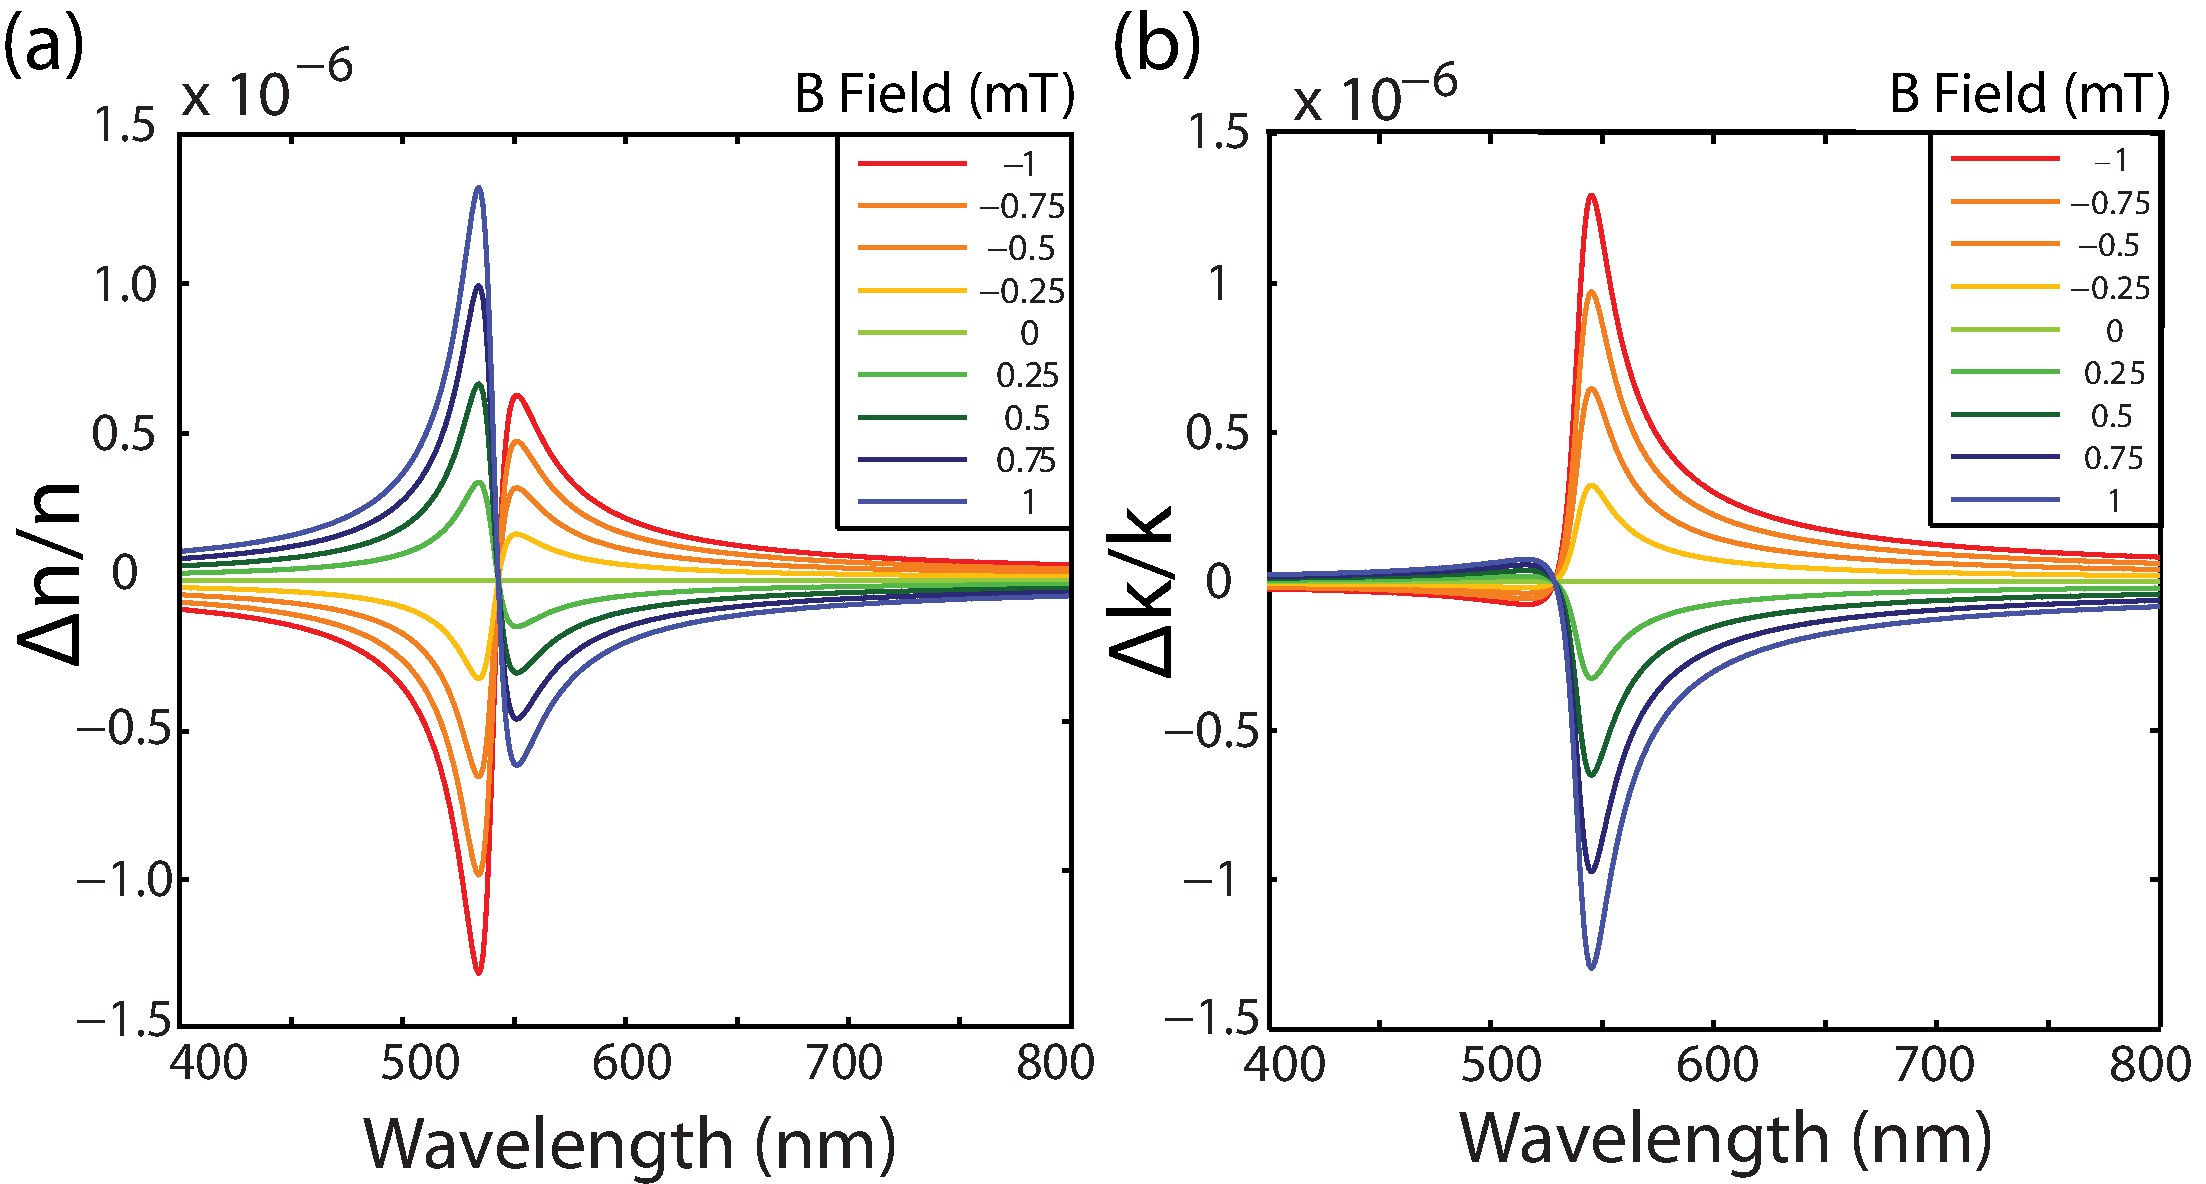
\includegraphics[width=\textwidth]{dnk_mT.pdf}
\caption{Relative MO shift of bulk gold when external fields are varied. (a) Real and (b) imaginary parts of the refractive index as a function of wavelength under illumination of 1 W/cm$^2$ RHCP when magnetic fields are varied.}
\label{fig:1}
\end{figure}

As can be seen in Fig.~\ref{fig:1}, around the plasmon resonance (540 nm) there are significant shifts in the real and imaginary parts of the refractive index. This MO model explains the response from small magnetic-field perturbations, however is insufficient to explain the changes in optical properties at higher applied magnetic fields [\cite{Singh}]. The MO response of noble metals (calculated with linear dynamics) is significantly smaller compared to that which occurs with ferromagnets in part because the difference between the cyclotron and plasma frequencies is orders of magnitude apart [\cite{Schnatterly}]. Moreover, the MO response depends on other factors such as the exchange interaction, specific band structure and spin-orbit coupling that allow ferromagnetic materials to have a greater MO response than noble metals [\cite{Armelles2}].  
\section{Nonlinear dynamics}
\subsection{Nonlinear current density}
In departure from prior investigations of MO effects on nanostructures, an analytical expression derived from the continuity equation [\cite{Hertel}] describes a time-averaged solenoidal magnetization current density:
\begin{equation}
\langle \vec{j_m} \rangle = \frac{i}{4q\langle \eta\rangle \omega}\nabla \times\big(\sigma_0^*\vec{E}^*\times\sigma_0\vec{E}\big),
\label{jm_eqn}
\end{equation}
where $\langle \eta\rangle$ is the time-averaged electron density, $\sigma_0$ is the specific conductivity of gold, and $\vec{E}$ is the total electric field at the surface. As seen in Eq.~\ref{jm_eqn} $\langle\vec{j_m}\rangle$ is polarization-dependent in its direction and magnitude. For a circularly-polarized $\vec{E}$ the term $\vec{E_{\pm}}\times\vec{E_{\pm}^*}$ becomes $\pm i |\vec{E_0}|^2\hat{z}$ and for a linearly-polarized field this term is zero. Note that $\langle\vec{j_m}\rangle$ scales inversely with $\langle \eta\rangle$, which may explain MO effects in non-metallic nanostructures [\cite{Kuznetsov}] and also scales with the intensity, in contrast to linear currents which scale with the electric field ($\vec{j}=\sigma_0\vec{E}$). 
\subsection{Nonlinear magnetization}
In this study of nanospheres, the time-averaged nonlinear current density is significant only in the azimuthal direction, $\hat{\phi}$, $\langle\vec{j_{m,r}}\rangle=0$, $\langle\vec{j_{m,\theta}}\rangle\ll \langle\vec{j_{m,\phi}}\rangle$. Although linear time-harmonic azimuthal currents exist, the current direction reverses every 1/2 cycle and time-average to zero. Since the nonlinear surface currents produce an anisotropic field-dependent perturbation to the specific conductivity, it is reasonable to employ a formalism similar to that used for the nonlinear polarization with the nonlinear current density as $\vec{j_p}(\vec{E}) = \vec{j^{(1)}_p}(\vec{E}) + \vec{j^{(2)}_p}(\vec{E},\vec{E}) + ... = \sigma_{p,r}^{(1)}E_q+\sigma_{p,r,s}^{(2)}E_rE_s+...$, where $\sigma^{(1)}_{p,r}$ is the specific conductivity in isotropic media. 
Using Eq.~\ref{jm_eqn} and Levi-Cevita notation $\sigma_{p,r,s}^{(2)}$ can be written as a third-rank tensor in the form:
\begin{equation}
\sigma_{p,r,s}^{(2)} = \frac{i|\sigma_0|^2}{4q\langle\eta\rangle\omega}\frac{\epsilon_{p,r,s} \hat{\partial_r}\epsilon_{s,t,u}E_t^*E_u}{E_{r}E_{s}}.
\label{DelSig}
\end{equation}
A relation for the induced magnetization can also be obtained using $\vec{j_m} = \nabla\times\vec{M}$, such that:
\begin{equation}
\vec{M_p} = \frac{i|\sigma_0|^2}{4q\langle\eta\rangle\omega}\epsilon_{p,r,s} E_{r}^*E_{s}
\end{equation}
\begin{figure}[b!]
\centering
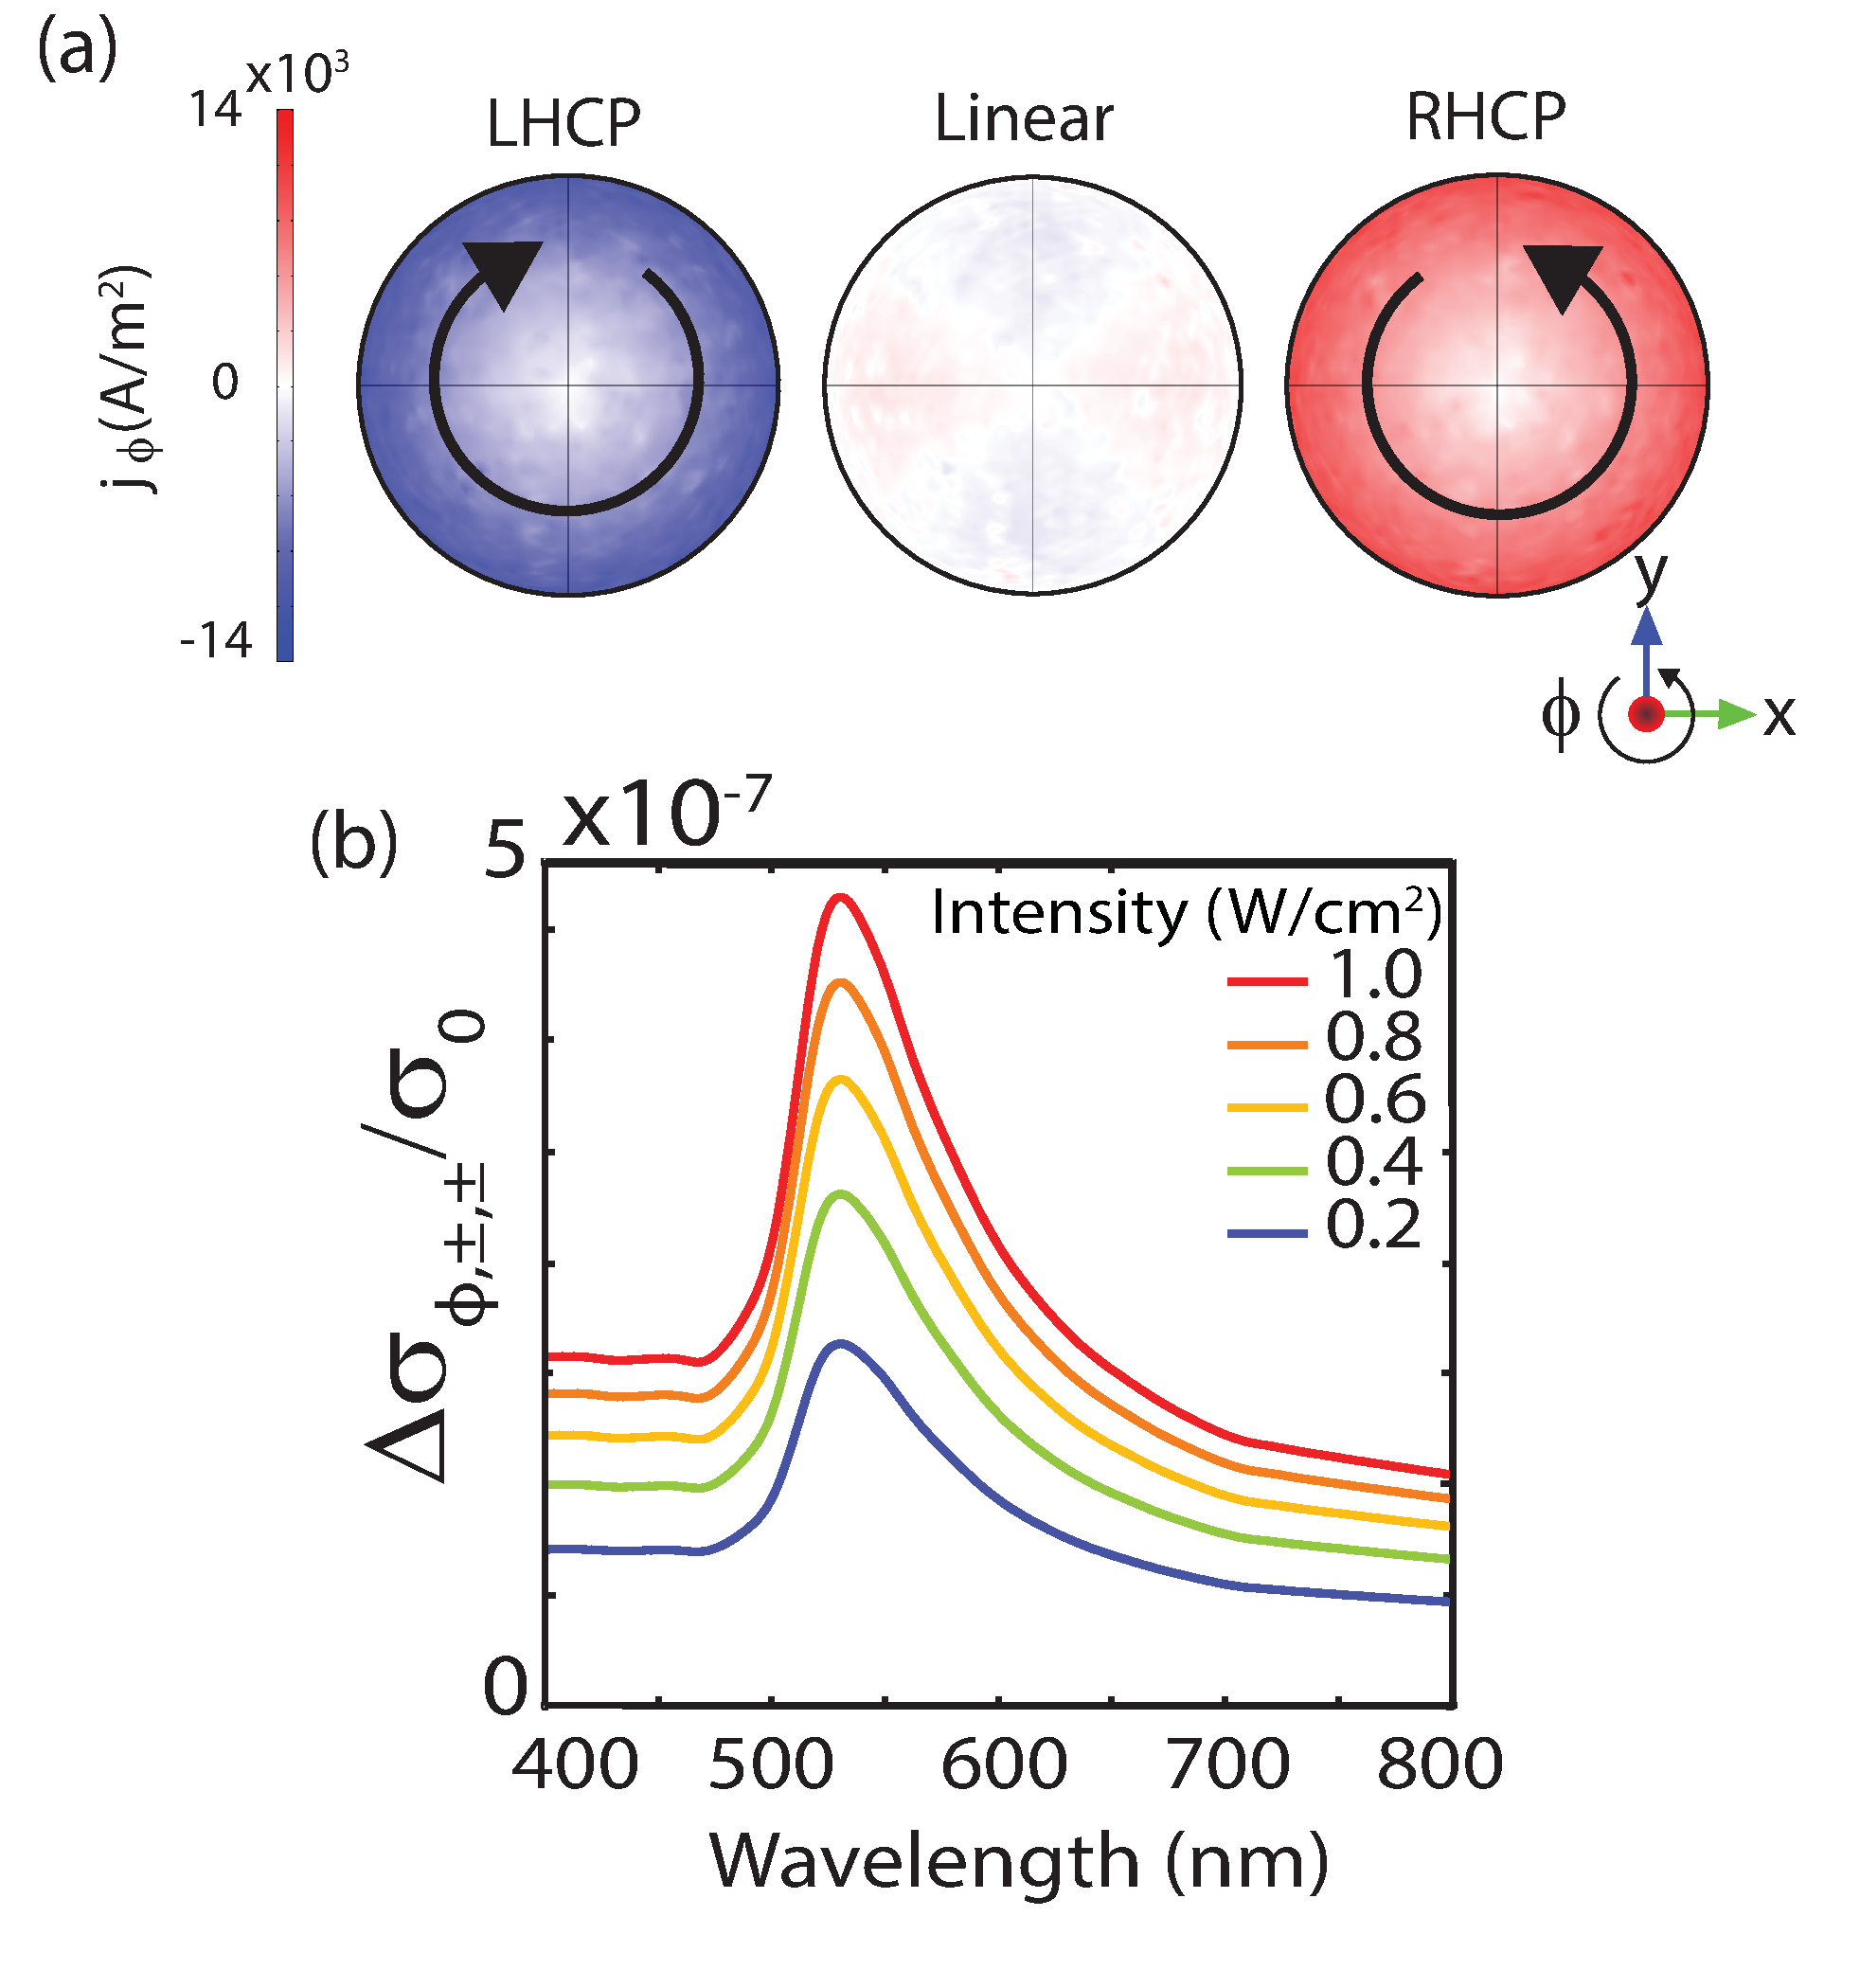
\includegraphics[width=0.95\textwidth]{SigandJPhi8}
\caption{(a) Surface plots of the nonlinear current density of an aqueous 80-nm gold nanosphere when illuminated by LHCP, linearly-polarized and RHCP light in the $\hat{z}$ direction at the plasmon resonance, 540 nm, at 1 W/cm$^2$. (b) Volume-averaged relative change in azimuthal component of the conductivity as a function of wavelength when illumination intensity is varied for RHCP or LHCP.}
\label{fig:2}
\end{figure}
\section{Numerical predictions}
\subsection{Finite-element simulation results}
\indent Numerical, finite-element simulations illustrate the strong polarization dependence of the nonlinear current density that the theoretical analyses predict. As seen in Fig.~\ref{fig:2}(a) the induced nonlinear current density, $\langle\vec{j_{m,\phi}}\rangle$, is calculated for an aqueous 80-nm gold nanosphere illuminated in the $\hat{z}$ direction with different polarizations. To simplify the notation of the nonlinear conductivity response only the first subscript of $\sigma^{(2)}$ that denotes the direction of the anisotropic change. It can be shown that $\sigma^{(2)}$ is nonzero only for curvilinear coordinates such as $\phi$ or $\theta$ in spherical coordinates. The numerical calculations illustrate that $\sigma^{(2)}_{\phi}$ is negligible for incident linear polarization, and RHCP and LHCP yield the greatest $\sigma^{(2)}_{\phi}$ with equal direction and magnitude; as illustrated in Fig.~\ref{fig:2}(b), as the light intensity increases, the conductivity of the nanoparticle also increases uniformly across wavelengths for both RHCP and LHCP. Since both the azimuthal currents ($\propto \nabla\times\vec{E}^*\times\vec{E}$) and the electric-field components ($\vec{E}_\phi$) reverse direction with polarization handedness, by symmetry, the relative changes in the conductivity tensor are identical for both RHCP and LHCP. 

\section{Experimental observation}
\subsection{Observation of transition from linear to nonlinear dynamics}
\begin{figure}[p]
\centering
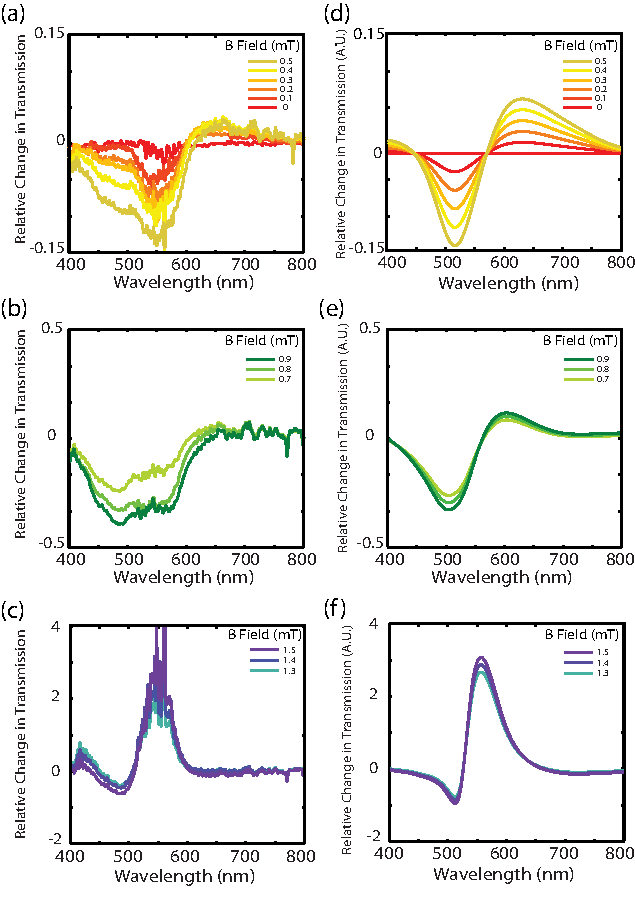
\includegraphics[height=0.95\textheight]{ExExpB11.pdf}
\caption{(Continued on the following page.)}
\label{Exp}
\end{figure}
\addtocounter{figure}{-1}
\begin{figure} [t!]
  \caption{(Previous page.) Normalized MO changes in transmission for aqueous gold nanocolloid at (a) low magnetic fields (b) intermediate magnetic fields and (c) higher magnetic fields. Theoretical MO change in transmission of aqueous 80-nm gold nanospheres in the (d) linear and (f) nonlinear analyses. Theoretical MO changes that combine the linear and nonlinear analyses are shown in (e) for intermediate magnetic fields. In all plots the illumination is 1 W/cm$^2$ and RHCP.}%missing
\end{figure}

\indent Experimental data of relative MO changes in transmission spectra are illustrated in Fig.~\ref{Exp}, alongside analytical results. The experiments were performed with samples of 0.05 mg/mL 80-nm poly-vinyl pyrolidone(PVP)-capped gold nanoparticles dispersed in aqueous solution (2.5$\times 10^{-6}$ fill factor). A solar simulator, polymer thin-film linear polarizer, and 400-800 nm achromatic quarter-wave plate produce RHCP white light, and a Helmholtz coil generates a uniform magnetic field in the direction of light propagation around the sample. A CCD spectrometer that captures the extinction spectra is placed behind a 0.5-cm optical path length cuvette containing samples.
\\\indent The dominant response is dependent on the illuminating light polarization at low magnetic fields and is polarization-independent in the presence of higher magnetic fields; a threshold behaviour exists. Experimentally, a magnetic field of 0.9 mT is associated as the bound between the linear (polarization-dependent) and nonlinear (polarization-independent) dynamics. The experimental data [Fig.~\ref{Exp}(a-c)] shows relative transmission data for RHCP and positive magnetic fields. Below the threshold, differences between the handedness of the polarizations are observed; the MO response is approximately equal and opposite in magnitude. Above, the transmission is similar for both RHCP and LHCP. 
\\\indent The experimental data agrees with analytical theory when the changes of the refractive index [Fig.~\ref{fig:1}] and conductivity [Fig.~\ref{fig:2}(b)] are incorporated to Mie theory [\cite{Mie}] and the corresponding relative changes in extinction spectra are computed. These calculated linear and nonlinear MO responses are shown separately in Fig.~\ref{Exp}(d) and Fig.~\ref{Exp}(f) respectively, and both linear and nonlinear MO responses are incorporated to analyse the total response at intermediate fields near the threshold [Fig.~\ref{Exp}(e)]. The relative change in the nonlinear MO response has been scaled to reflect the experimental behaviour. The nonlinear response is modelled as a function of the external magnetic field, which tunes the strength of the coupling that causes the MO response. The threshold behaviour observed experimentally is expected to occur when the theoretical linear and nonlinear effects are comparable. Moreover, this theoretical model provides excellent quantitative agreement; in this analysis of a single nanosphere the changes in the refractive index and conductivity via the linear and nonlinear responses are of similar magnitude with 1-W/cm$^2$ illumination intensities and 1-mT magnetic fields. The transition between the polarization-dependent linear response and the polarization-independent nonlinear response occurs when either the magnetic field strength or the intensity of light is varied.
\section{Discussion}
\subsection{Magnetization magnitudes}
\indent The understanding of the light scattering at nanostructures is crucial for understanding both linear and nonlinear MO effects. In the limit of thin structures, the scattered component of the electric field is largest in the longitudinal direction, $E_z$, and carries phase singularities that change with circular polarization handedness [\cite{Vuong,Hasman}]. The locations of the phase singularities, as well as the topological charges themselves vary with nanostructure geometry and are associated with the loops in the {\it linear} current density. \textit{Nonlinear} current loops are also produced by scattering events that induce surface charge densities, which couple with the incident fields [Eq.~\ref{jm_eqn}]. It is these nonlinear nonzero time-averaged current loops that lead to the material magnetization $M_z$. The amplitude and phase of $E_z$ and corresponding $M_z$ for an 80-nm gold nanosphere illuminated with RHCP are shown in Fig.~\ref{Ez}. Although the non-magnetic nanoparticle magnetizations are small compared to that of a ferromagnet (10$^5$ times smaller) due to masses on the order 10$^{-18}$ kg, the subsequent mechanical motion becomes significant.
\begin{figure}[t!]
\centering
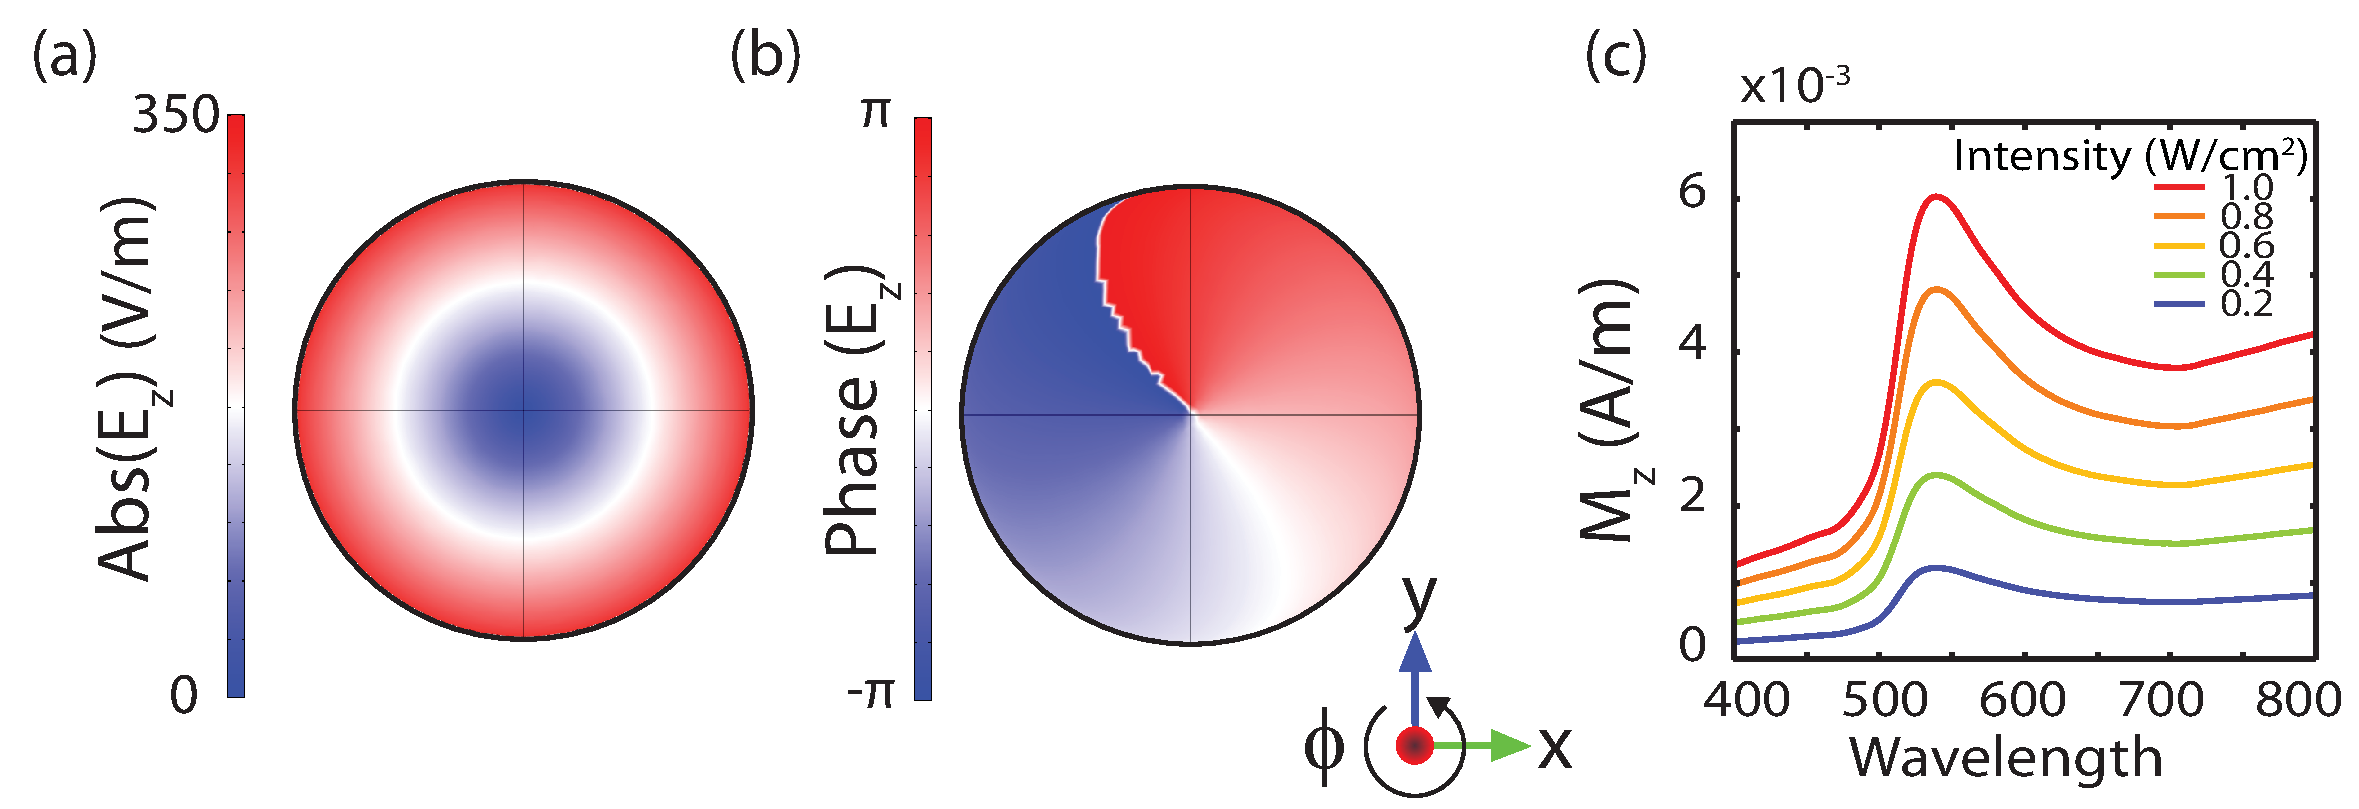
\includegraphics[width=0.95\textwidth]{EzMz}
\caption{Numerically calculated (a) amplitude and (b) phase of the longitudinal component of the electric field, $E_z$, with 540-nm 1 W/cm$^2$ RHCP illumination intensity. (c) Volume-averaged magnetization as a function of wavelength when illumination intensities are varied. All plots are for an aqueous 80-nm gold nanoparticle.}
\label{Ez}
\end{figure}

\subsection{Time-dependent response}
\indent The delayed optical response to an applied magnetic field is likely the result of the settling motion of non-spherical nanoparticles and nanoclusters. Aggregates often form as a result of random Brownian motion and magnetic-dipole interactions, so they are considered in this analysis. Also acknowledged are irregularities in the nanoparticles employed in the experiments-- they are not perfect spheres due to the fabrication process. Such variations from spherical geometry cause magnetization differences that depend on the nanoparticle orientation with respect to the electric field.
\\\indent Changes in extinction spectra reflect the magnetization associated with the nanoparticle and nanoclusters reorientation. Structural anisotropy and orientation affect the magnetization of the nanoparticle, which is illustrated with dimer nanoclusters and ellipsoids of different aspect ratios. As can be seen in Fig.~\ref{Dimer}(a) there is a reduction in the magnetization by almost 50\% as a dimer nanocluster rotates from minimal to maximal incident surface area with respect to electric field.
 The relative change in the magnetization is shown in Fig.~\ref{Dimer}(b) as a function of aspect ratio when ellipsoidal nanoparticles of equal volume are rotated from minimal to maximal incident surface area. Ellipsoids with aspect ratio 1 (spheres), exhibit no difference as they are rotated, and greater differences are observed when the aspect ratio increases. To guide the eye, a trendline that reflects the Biot-Savart law is provided in Fig.~\ref{Dimer}(b). Deviations from the trendline are attributed to changes in the plasmonic eigenfrequency. Regardless, anisotropy in the nanoparticle shape leads to MO magnetization that varies with the orientation, a concept in agreement with prior work~\cite{Jain,Funston}. 
\\\indent %Numerical simulations of dimer nanoclusters and ellipsoids indicate that structural anisotropy lead experimentally to torque forces that maximise MO and mechanical effects.
There exists a nanoparticle/nanocluster orientation with respect to the external magnetic field that maximises $\langle\vec{j_m}\rangle$. 
\begin{figure}[t]
\centering
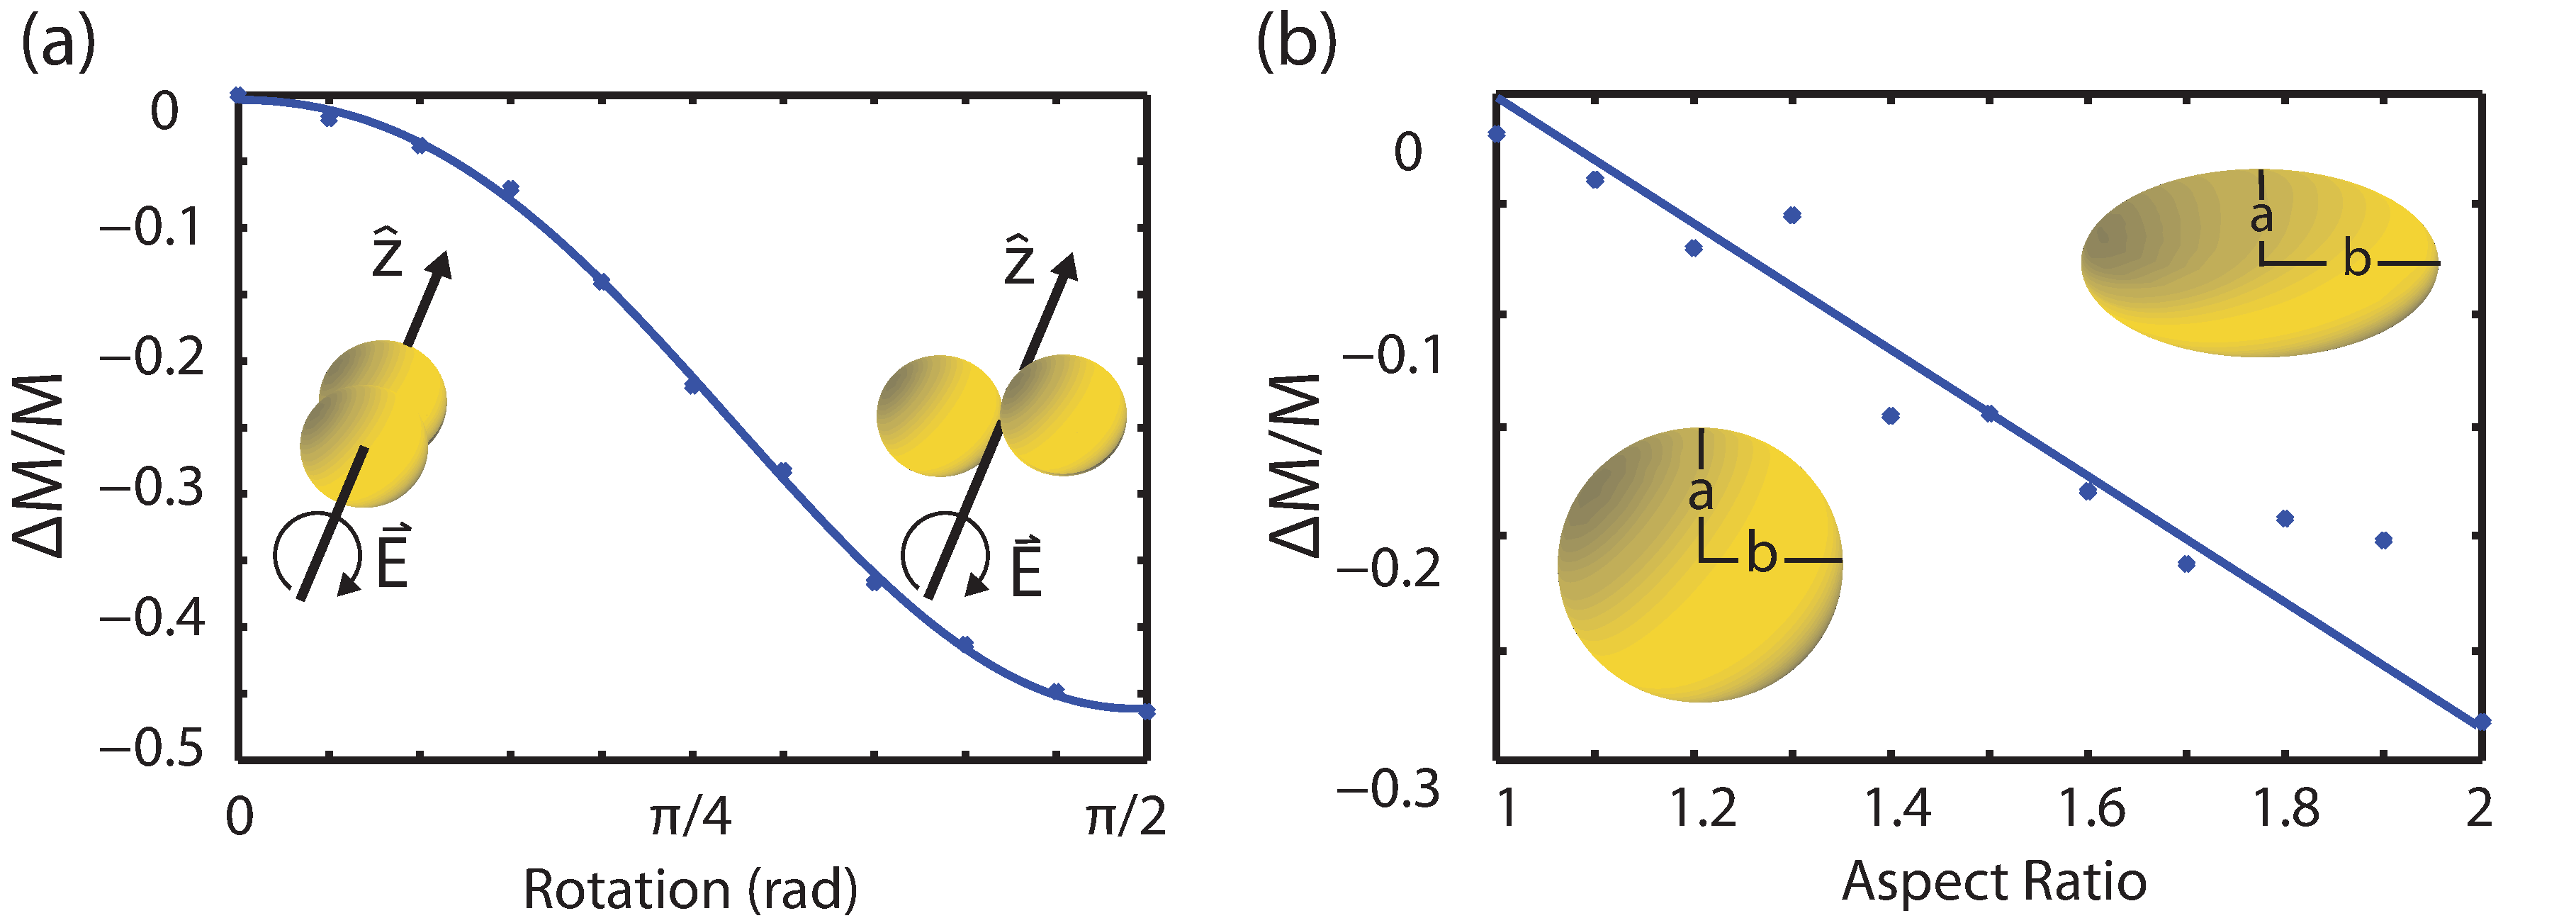
\includegraphics[width=0.95\textwidth]{MagPlots}
\caption{Numerically calculated relative change in magnetization (a) of a 80-nm gold dimer nanocluster as a function of angle of rotation, and (b) ellipsoidal gold nanoparticle rotated from minimal to maximal surface area as a function of aspect ratio, illuminated with 540-nm 1 W/cm$^2$ RHCP.}
\label{Dimer}
\end{figure}
The system is expected to stabilize in an orientation that maximises the nanoparticle magnetization. The nanocolloid magnetization is largest at the plasmon resonance when the local electric field and scattering is maximised.
\\\indent Yet, scattering dynamics present a complex dynamical system that is not fully understood in the context of MO responses. Autocorrelation data reveals significant pulse broadening through gold nanocolloid solution that scales with the square of the sample thickness that suggests a strong scattering [\cite{Genack}] despite low fill factors (2.5$\times 10^{-6}$). 
%The scattering cross-sections of metal nanocolloids are much greater than their geometrical cross-section at resonance~\cite{Mie}, and 5 orders than the light emission from strongly fluorescing dyes~\cite{Jain2}, indicating a strongly scattering medium. %Autocorrelation data shows significant pulse broadening through 400 $\mu$m of nanocolloid solution from 2.3 ps to 3.2 ps, which suggest appreciable multiple scattering events, despite low fill factors (2.5$\times 10^{-6}$). 
Another possibility for the larger-than-expected results is diffractive coupling between nanoparticles that can exhibit strong long-range interaction [\cite{Barnes2}] that lead to near-field enhancements, which are anticipated to increase in a 3-D matrix. The material properties of the matrix also influence the MO response. For instance, the presence of any ions or charged particles, common in solvents such as water, modifies the electrodynamics of the system, which subsequently influences the MO response of the system.
\section{Conclusion}
\indent This chapter demonstrates the observation of MO responses in non-magnetic nanocolloids at ultra-low illumination intensities and magnetic fields. Metal nanocolloids are magnetized and the optical properties are shifted when excited by coincident elliptically-polarized electric fields and DC magnetic fields. Experimentally-observed extinction spectra are in good agreement with predictions of linear and nonlinear MO effects and new considerations are provided for novel mechanical effects that were previously considered unattainable. A theoretical model is demonstrated that successfully explains the transition between linear and nonlinear MO plasmon dynamics of metal nanoparticles. This chapter provides the theoretical framework to study MO responses in non-magnetic nanostructures. In particular, new methods to identify, optically self-assemble and magnetically torque large quantities of disperse, non-spherical nanoparticles with broadband light sources are realized.

\section{Experimental difficulties and future work}
The experimental procedure to study the transmission properties were quite difficult. One recurrent issue that occurred was a time dependence in the transmission properties before any magnetic field was applied. This issue was attributed to thermal stabilization of the system and was overcome by waiting for the transmission properties to thermally stabilize before turning on the magnetic field and taking any measurements.

Care was also taken in the amount of light intensity, as it was found that if the light intensity was too great, there would be aggregation and settling of the nanoparticles at the bottom of the substrate. Aggregation may affect the results by shifting the plasmonic resonance of the nanoparticles due to the increase in size, which may confound the results. Settling of the nanoparticles is also undesirable since there is a reduction of the nanoparticle density interacting with the electric and magnetic fields that way decrease the MO effect and increase the transmission through the sample, confounding the results.

Future work on this subject may involve a deeper investigation of the threshold between the linear and nonlinear components that cause the respective transmission properties. Further work in this field may incorporate how plasmonic capping agents such as PVP may influence the magneto-optical responses. The electrostatic capping agents that are responsible for keeping the nanoparticles separated may influence the magneto-optical response by acting as a charge transfer complex. Lin et al. showed that when carbon nanotubes are bonded to a metal-to-ligand charge transfer complex, the resulting nanotubes exhibit magneto-optical responses when exposed to visible light [\cite{Lin:2015}]. 
\clearpage

% chapter three
\chapter{Plasmon-induced Lorentz forces of nanowire chiral hybrid modes}
\chaptermark{Lorentz forces of nanowire chiral hybrid modes}
\section{Introduction}
While light is massless, it imparts momenta that are significant, which: confine ion beams [\cite{Petrich1993}]; propel solar sails [\cite{Janhunen2007}]; rotate and twist objects [\cite{Beth1936, Paterson2001, Tsai2014}]; levitate, trap, and move matter [\cite{Laboratories1997, NieminenRev, Novotny1997}]; cool atoms [\cite{Weiner1999}]; and alter the crystallization of solids [\cite{Chowdhury1985}]. Our knowledge of light's momentum transfer is intrinsic to the design of facilities for low-temperature and high-energy physics, cell and molecular biology, and advanced materials research [\cite{Laboratories1997}], and is relevant to an expansive development of optomechanical devices for sensors and electronics technologies [\cite{Hugel2002, Kippenberg2007, Thourhout2010}].  Currently, the laser trapping of uncharged dielectric matter is commonplace [\cite{Laboratories1997}]; however, the optically-induced mechanics of conducting or plasmonic nanoparticles have been shown to be, at the very least, more complex [\cite{Dienerowitz2008, Saija2009, Shvedov2010, Yan2012, Yan2012a, Yan2013, Yan2013a, Yan2013b}]. One challenge stems from the numerous channels through which energy is transferred: particles also move in the presence of electric fields, magnetic fields, and thermal gradients [\cite{Bhatt, Keshoju, Edwards2006}], which are directly and indirectly produced by plasmons.  Understanding these dynamic, momentum-conserving mechanisms involves, in part, understanding the interactions among these fields.


Theoretical considerations of the gradient-intensity trapping forces, radiation pressure forces, and induced-electric-dipole interactions [\cite{Laboratories1997}] are insufficient for predicting the optomechanical behavior of plasmonic nanoparticles.  It is increasingly apparent that the excitation of plasmons play a critical role in the optically-induced movement of nonspherical nanoparticles [\cite{Yan2013}]. For example, a model of the induced electric dipole with an electric field only predicts that silver nanorods will align parallel to the direction of the illuminating linear polarization of light [\cite{Tong}], and that nanowires rotate continuously in the presence of circularly-polarized light or optical vortices via the transfer of spin or orbital angular momentum, respectively [\cite{Yan2013a, Lehmuskero1, Lehmuskero:14}]. However, this theoretical model that considers the nanoparticle polarizability alone cannot discriminate between the different mechanical behaviors associated with different nanorod-ends and particle aspect ratios [\cite{Tong}].  Nanoparticle geometry often dictates local surface plasmon modes [\cite{Knight2007}]; further insight into the physical phenomena that underlie the optomechanical behavior of non-spherical plasmonic particles is necessary.

This chapter investigates the Lorentz forces strictly attributed to surface plasmons on metal nanowires, which are of wide technological interest [\cite{Knight2007, Lal2007, Maier2005}], and potentially relevant to other plasmonic nanostructures such as carbon nanotubes, where similar chiral plasmonic behavior is tunable from the UV to THz [\cite{PhysRevBnanotube}]. The first successful trapping of a nanowire in a 3D optical trap identified an important role of plasmons. Yan, {\it et al.,} demonstrate that gold nanowires---but significantly, {\it not} silver nanowires---are confined by a Gaussian-beam optical trap [\cite{Yan2013}].  Yan proposes that the macroscopic perspective of optical trapping is insufficient and should be replaced with a plasmonic model [\cite{Yan2012}] and identifies asymmetric modes with trapping instabilities; nevertheless, a simple model that connects the dynamic instability of nanowires with its plasmonic behavior has not yet been advanced.

Plasmonically-induced Lorentz forces that are produced on gold nanowires by the illumination of linearly-polarized electromagnetic plane waves are investigated via numerical simulation.  The plasmonically-induced forces are significant in chiral geometries and when chiral hybrid plasmonic modes [\cite{Zhang2011}] are present.  This chapter identifies the electromagnetic torque and compression on the nanowires associated with the surface currents and asymmetric time-averaged fields. The results identify significant mechanical forces produced by surface plasmons in chiral hybrid modes that are currently neglected. Plasmonically-induced Lorentz forces are even expected to critically prevent the stable optical trapping of conducting nanowires, particularly when longer trapping-laser wavelengths {\it between} strong absorption resonances are employed. The approach highlights a critical dependence of nanoparticle shape [\cite{Knight2007, Tong}] and plasmon relaxation [\cite{Yan2013}] on the optically-induced forces, and considerations are relevant to future microfluidic applications.

This chapter is organized as follows. In Sec.~\ref{intro} the chiral geometry of our system is described, the numerical computations associated with Lorentz forces are outlined, and the asymmetric surface plasmon modes is illustrated. The electric dipole and plasmonic Lorentz forces of nanowires that are aligned in the transverse plane are evaluated, and agree with and clarify prior experimental results. In Sec.~\ref{forces}, the axial and translation forces associated with surface plasmons are described, these forces are generally stronger than those associated with electric dipoles.  In Sec.~\ref{3D} an analysis of the torque forces that arise from the 3D scattering is provided.  Analysis in this chapter ignores any nonlinear responses that may arise due to heat [\cite{Shvedov2010}], steam [\cite{Saija2009, Fang2013}], the electrochemical response of solvent [\cite{Arcenegui2013}], and nonlinear magneto-optical effects [\cite{Singh, Moocarme2014}], although these effects are not negligible, particularly at high illumination intensities.  Surface effects that may arise in the interaction between nanoparticles due to coatings or interfaces are also ignored, however this work is highly relevant to the understanding of such interactions with plasmonic materials [\cite{Bonin}].  The mechanical translation, compression, and torque forces associated with the plasmonic surface currents are significant and interfere with the optical trapping of elongated nanoparticles. The results in this chapter indicate that there exists a frequency cut-off at which the chiral plasmon excitation is minimized; avoiding chiral plasmon excitation will provide greater trapping stability.

\section{Setup and simulations of 2D dynamics}\label{intro}
\subsection{Calculation of electromagnetic fields}
\begin{figure}[ht]
\centering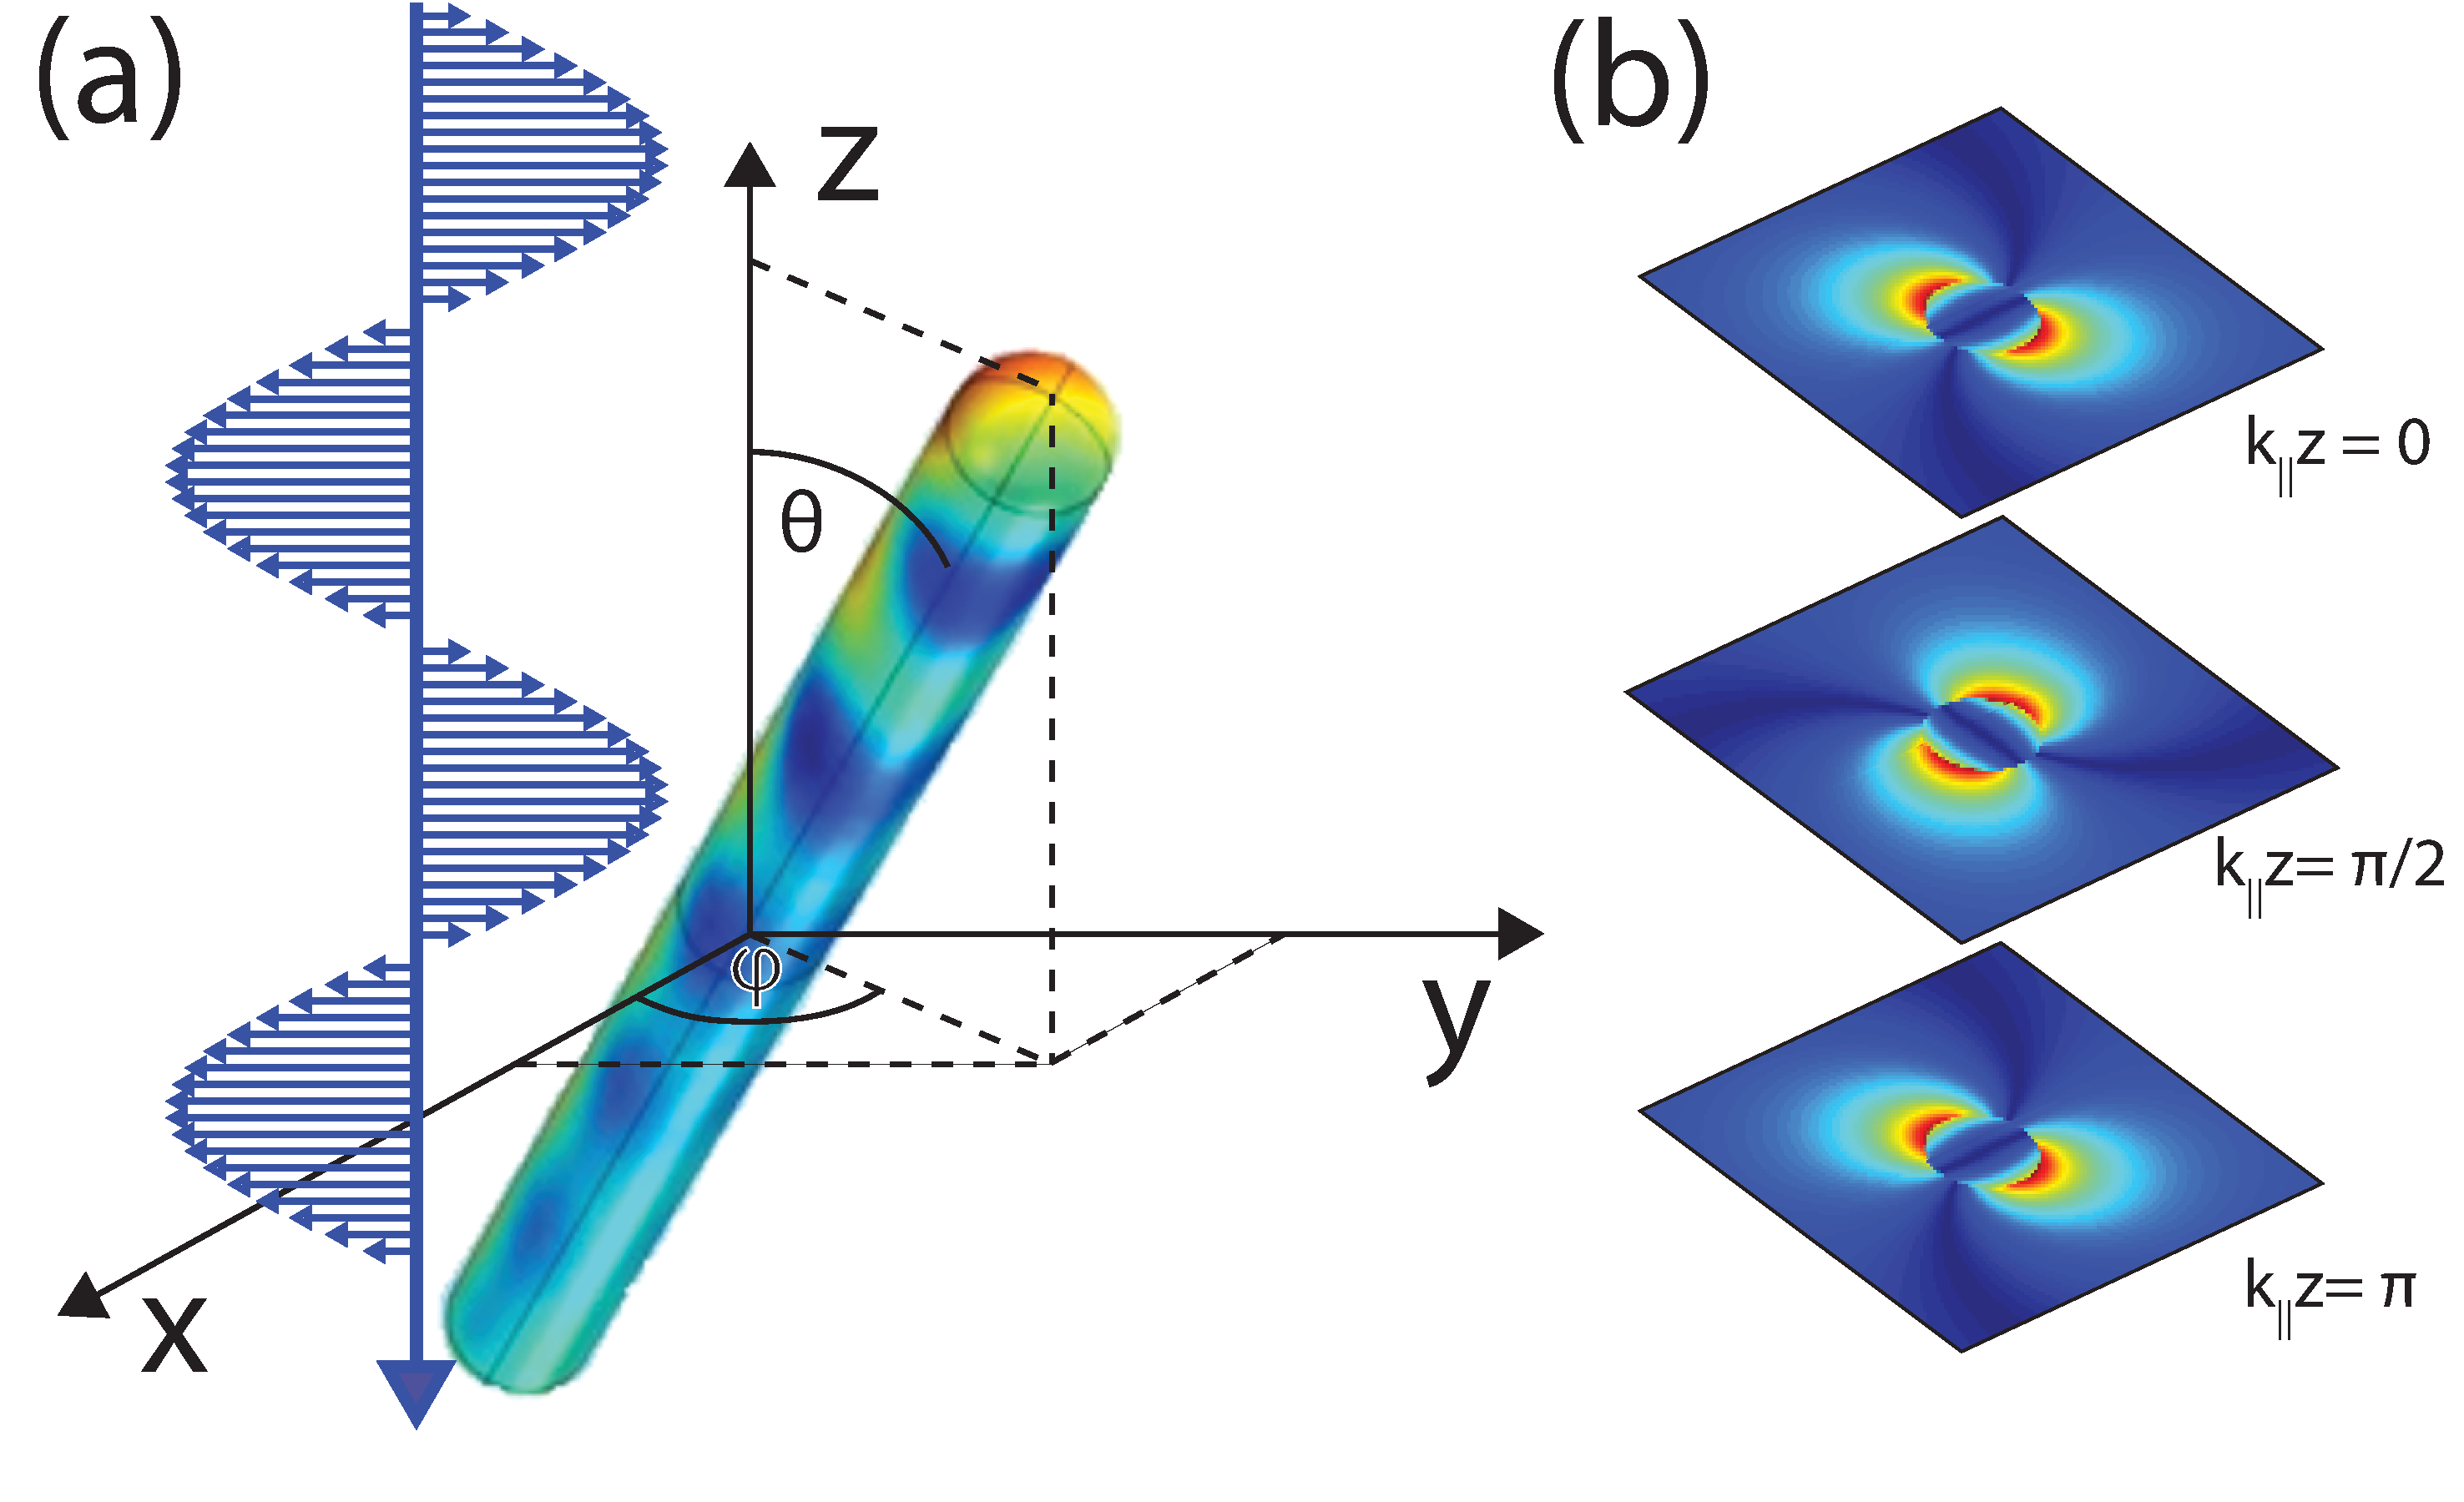
\includegraphics[width=0.95\textwidth]{SetupPicMatt.pdf}
\caption{(a) System geometry: a gold nanowire (75-nm diameter, rounded-cap, 1025-nm length) is aligned about spherical coordinates $\theta$ and $\phi$, and a $y$-polarized electromagnetic wave (1 W$/$cm$^2$) travels in the $-z$ direction. (b) The electric field profile surrounding a nanowire resulting from superposed angular momentum modes $m=0,\pm1$ with propagation lengths
$k_{\parallel}z = 0$, $\pi/2$, and $\pi$.\label{setup}}
\end{figure}

In the numerical investigation (COMSOL v4.3a, RF module, $\sim$2 million degrees of freedom), a linearly-polarized plane wave illuminates a gold nanowire immersed in deionized water, whose orientation is determined by $\theta$ and $\phi$, as illustrated in Fig. \ref{setup}(a). The nanowire dimensions are fixed with 75-nm diameter, and 950-nm length.  The nanowire terminations are hemispherical, thus the nanowire measures 1025-nm end-to-end.
%We use rounded terminations which couple the modes differently compared to flat terminations via mode-match conditions~\cite{Li2010} .
 The electromagnetic waves are polarized in the $y$-direction and propagate in the negative-$z$ direction.

In particular, this chapter focuses on the dynamics that occur when the wire is tilted towards the incoming plane wave, i.e., $\theta \neq 90^\circ$. Such arrangements produce chiral plasmons, which are superpositions of the transverse and longitudinal modes.  The signature for such modes is a time-averaged electric-field amplitude on the surface of the nanowire that varies azimuthally and over the length of the sample, a result of the superposition of two or more plasmon modes with varying azimuthal angular momentum number $m$, which are excited simultaneously by the incident fields.  The phase difference associated with the different angular momentum numbers $m$ determines the asymmetric nanowire intensity patterns [\cite{Zhang2011}]. In cylindrical coordinates the electromagnetic fields take the form [\cite{Chang2007}]:

\begin{eqnarray}\label{Efield}
E_j(r) = \frac{1}{k_j}& \sum_m&\Big\{\big[\frac{m}{s}a_{j,m}F_{j,m}+\frac{k^{(\parallel)}_{m}k^{(\perp)}_{j ,m}}{k_j}b_{j,m}F_{j,m}'\big]i\hat{s}\nonumber \\
  &-&\big[{k_{j ,m}^{(\perp)}}a_{j,m}F_{j,m}'+\frac{mk^{(\parallel)}_{m}}{k_js}b_{j,m}F_{j,m}\big]\hat{\phi} \\
  &+& \frac{[k^{(\perp)}_{j ,m}]^2}{k_j}b_{j,m}F_{j,m}\hat{z}\Big\}e^{ik^{(\parallel)}_{m}z+im\phi} \nonumber
\end{eqnarray}



\begin{eqnarray}\label{Hfield}
H_j(r) = \frac{i}{\omega\mu_0}&\sum_m &\Big\{\big[\frac{k^{(\parallel)}_{m}k_{j ,m}^{(\perp)}}{k_j}a_{j,m}F_{j,m}'+\frac{m}{s}b_{j,m}F_{j,m}\big]i\hat{s}\nonumber \\
&-&\big[\frac{mk^{(\parallel)}_{m}}{k_js}a_{j,m}F_{j,m}+{k_{j ,m}^{(\perp)}}F_{j,m}'\big]\hat{\phi}\\
&+&\frac{[k_{j ,m}^{(\perp)}]^2}{k_j}a_{j,m}F_{j,m}\hat{z}\Big\}e^{ik^{(\parallel)}_{m}z+im\phi}\nonumber
\end{eqnarray}
where $(s,\phi,z)$ are the cylindrical coordinates, the wave vectors are related by $\epsilon_jk_0^2=[k_{j ,m}^{(\perp)}]^2+[k^{(\parallel)}_m]^2$ where $\epsilon_j$ is the dielectric constant in region $j$ and $k_0$ is the wave vector in vacuum. $j=1$ outside the cylinder where $F_{1,m} = H_m (k_{1,m}^{(\perp)} s)$, the Hankel function of $m^{th}$ kind. $j=2$ inside the cylinder where $F_{2,m} = J_m(k_{2,m}^{(\perp)} s)$, the Bessel function of $m^{th}$ kind, and primes denote derivatives with respect to the argument. $a_{j,m}$ and $b_{j,m}$ are constants determined by boundary conditions. The modes excited in this system are the $m=0$, TM$_0$ mode and two degenerate first order $m=\pm 1$ modes, HE$_{\pm 1}$. Specifically, chiral-hybrid modes occur when all three of the lower order modes are simultaneously excited \textit{and} there is a phase difference between the HE$_1$ and HE$_{-1}$ modes.
A superposition of the three lowest order modes, $|m|\leq 1$ are shown in Fig. \ref{setup}(b) at different cross-sections of the nanowire corresponding to $k^{(\parallel)}_1z = 0, \pi/2$, and $\pi$. In general, the patterns in the electromagnetic fields produced off-resonance correspond to a periodic, asymmetric pattern on the wire that neither carries mirror symmetry along the length nor across the width of the wire.  It is anticipated that this asymmetry, which arises from the chiral illumination geometry, that produces a net translation and torques via Lorentz forces.

\subsection{Calculation of Lorentz force}
The well-known Lorentz law, $\mathbf{f}_{Lorentz} = q(\mathbf{E} + [\mathbf{v} \times \mathbf{B}])$, governs the force on a charge $q$ with velocity $\mathbf{v}$ in the presence of electric and magnetic fields, $\mathbf{E}$ and $\mathbf{B}$. While it is true that displacement of a charged particle can be resolved to physical quantities such as dielectric function and plasma frequency the focus of our investigation is related the macroscopic movement of the nanowires.
Investigated in this chapter are the Lorentz forces that act on a free electron gas which is bound to the surface of the nanowire. Such forces arise from time-harmonic electric and magnetic fields and subsequently, the effects of time-harmonic charge densities and surface currents. The time-averaged macroscopic force density is rewritten:
\begin{eqnarray}
\big{<}\mathbf{f}_{Lorentz}\big{>}&=& \rho[\mathbf{E^*}+(\mathbf{v}\times\mathbf{B}^*)] + c.c. \\
&=& \epsilon_0(\nabla \cdot \mathbf{E})\mathbf{E}^* + \mathbf{J}\times\mathbf{B}^* + c.c. \label{fmic}\\
&=&\mathbf{f}_E + \mathbf{f}_M
\end{eqnarray}
where $\rho$ is the charge density, $\epsilon_0$ is the permittivity constant, and $c.c.$ refers to the complex conjugate. $\mathbf{J}$ is the current density and can be determined from the electric field [Eq.~\ref{Efield}] via the relation $\textbf{J} = \sigma\textbf{E}$. The volume-integrated terms of Eq.~\ref{fmic} yield separate effects.  The induced electric-dipole force, $\mathbf{f}_E$, depends on the polarizability of the material, which is also shape-dependent [\cite{Liaw}] while the Lorentz force associated with surface currents, $\mathbf{f}_M$, is the focus of this investigation.

\subsection{Calculation of torque forces}
Also studied are the net torque forces associated with Eq.~\ref{fmic} with respect to the origin and geometric nanowire center. The torque associated with $\mathbf{f}_M$ is numerically computed directly:
\begin{equation}
\mathbf{T}_M=\int_V \mathbf{r} \times \mathbf{f}_M dV,\label{Tm}
\end{equation}
whereas the time-averaged torque associated with the induced electric dipole is
\begin{equation}
\mathbf{T}_E=\int_V \mathbf{r} \times \mathbf{f}_E dV=\int_V \mathbf{P} \times \mathbf{E}^* dV+ c.c.,
\label{Te}
\end{equation}
where $\mathbf{P}$ is the polarization and $\mathbf{r}$ is the radial coordinate vector in spherical coordinates. Eq.~\ref{fmic}, \ref{Tm}, \ref{Te}, are calculated over the volume of the nanowire in the numerical simulations.

\begin{figure}[ht]
\centering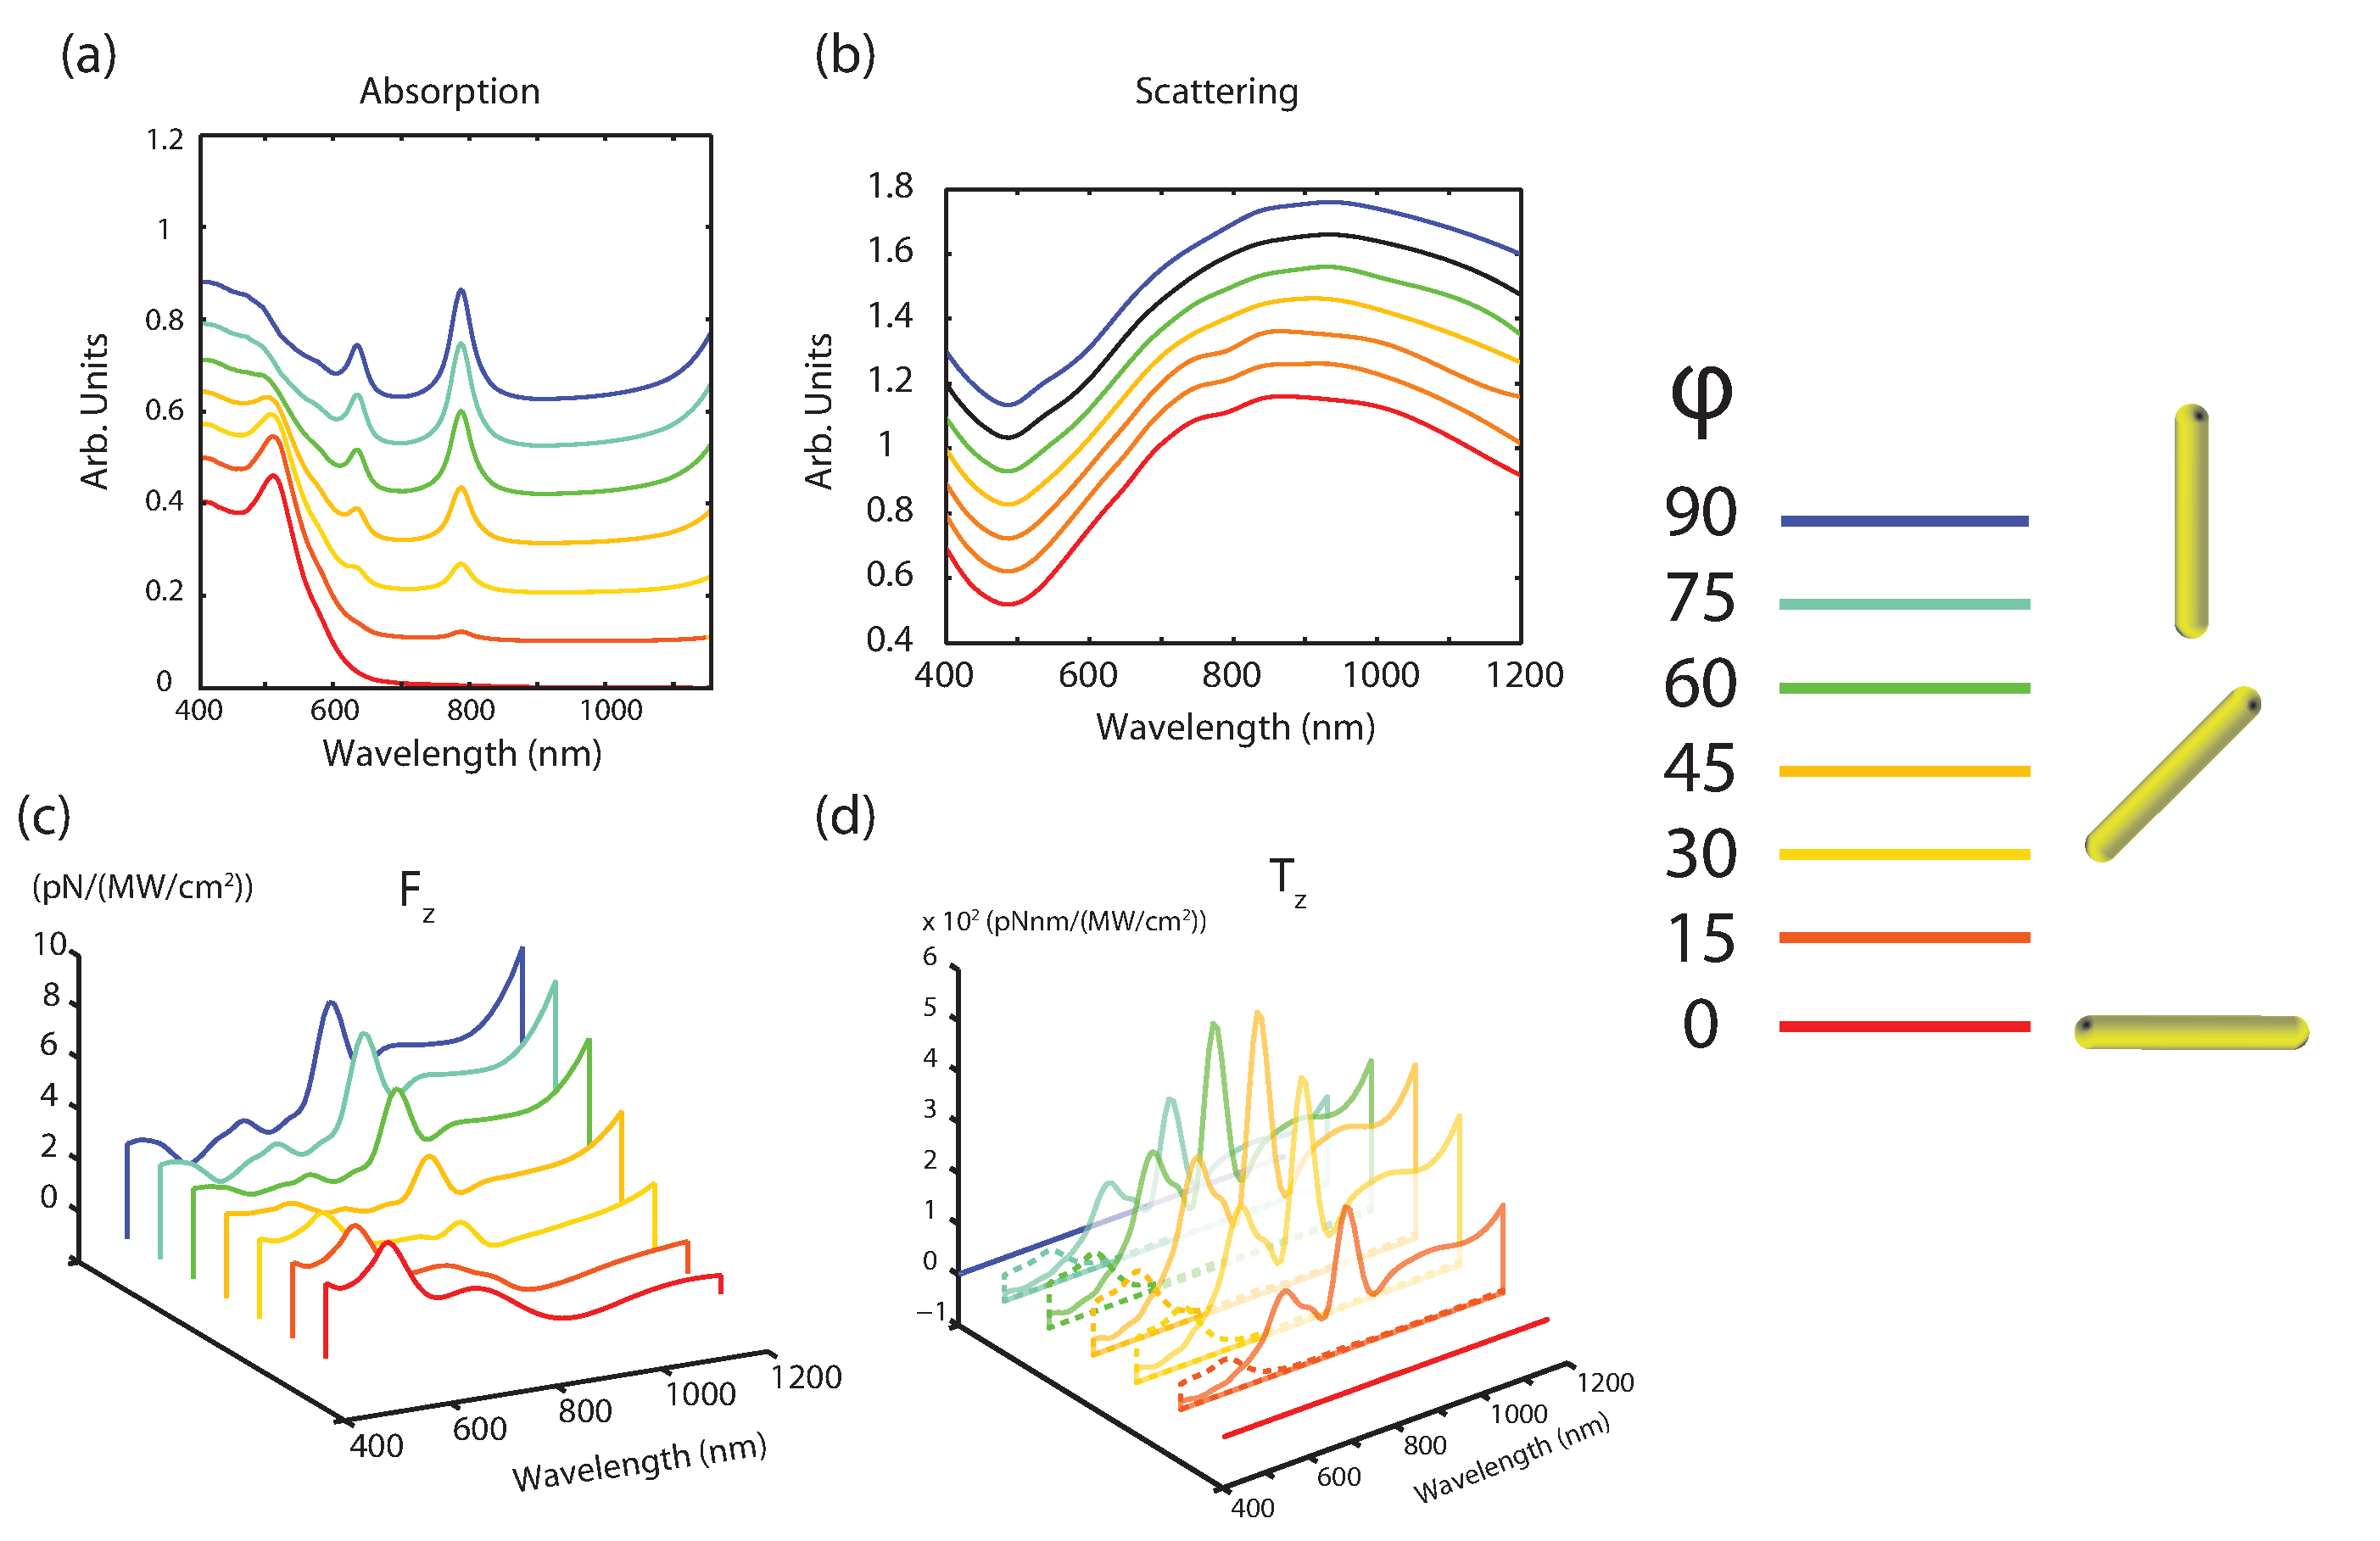
\includegraphics[width=\textwidth]{ScattAbsorptionF_zT_z.pdf}
\caption{Characteristics of a nanowire in the $x$-$y$ plane for varying orientation angle $\phi$ with $\theta = 90^\circ$. (a) Absorption cross-section. (b) Scattering cross-section, ((a), (b) spectra offset for clarity). (c) Net longitudinal force in the direction of light propagation, $-F_z$,  associated with the plasmonic Lorentz force. (d) In-plane torque $T_z$ produced by plasmons $\mathbf{f}_M$ (solid lines) and the induced electric dipole $\mathbf{f}_E$ (dashed lines).}\label{absorption}
\end{figure}

The study is introduced with a presentation of the well-studied plasmon-induced forces when the nanowire is normal to the incident electromagnetic wave, which represents the experiments performed when wires are pressed via radiation pressure along a normal surface such as a microscope slide in a 2-D trap [\cite{Tong}]. In this configuration, chiral plasmons are not produced; nevertheless, surface plasmons produce significant Lorentz forces.  Figure \ref{absorption}(a) shows the absorption cross-section for a nanowire in this transverse configuration. When the nanowire is aligned with the polarization of incident radiation ($\theta = 90^\circ, \phi = 90^\circ$), the longitudinal modes ($\lambda$ = 625nm, 790nm) are present; when it is aligned perpendicular ($\theta = 90^\circ, \phi = 0^\circ$), only the transverse mode ($\lambda$ = 510nm) is present.
% The nanowire hemispherical ends do not produce significant dispersion or shift in wavelength resonance with respect to nanowire rotation.

The longitudinal components of $\mathbf{f}_M$ are significant (on the order of pN/(MW/cm$^2$)) in the direction of light propagation ($-z$) when the transverse and longitudinal plasmonic resonances are present [Fig. \ref{absorption}(c)]. Large longitudinal forces arise between wavelengths $\lambda=$ 900-1100nm in which there is large scattering and low absorption [Fig. \ref{absorption}(a), (b)].
% At longer wavelengths, between longitudinal modes ($\lambda=$900-1100nm), the longitudinal force arising from plasmons is unexpected
When the wire is perpendicular to the light polarization ($\phi = 0^\circ$), the longitudinal force is positive and pointed in a direction {\it opposite} to the light propagation, in a manner that is reminiscent of optical tractor beams [\cite{Ruffner2012}]; when the wire is aligned parallel to the linear polarization of light ($\phi = 90^\circ$), the longitudinal force increases significantly. It has generally been assumed that radiation pressure produces the strong longitudinal forces of nanowires; that longitudinal forces are {\it also} produced via surface currents implies additional considerations and the importance of understanding plasmonic Lorentz forces.  Such plasmonic forces are strong even when there is minimal plasmonic absorption suggesting that the scattering off nanostructures plays a role.

Provided here is a comparison of the longitudinal components of $\mathbf{T}_E$ and $\mathbf{T}_M$ [Fig. \ref{absorption}(d)] which further points to the importance of plasmonically-induced Lorentz forces although the contributions are qualitatively similar in 2D.  Both torque terms are negligible when either $\phi = 0^\circ$ or $\phi = 90^\circ$ and both terms are largest at $\phi = 45^\circ$. The trends are in agreement with prior experimental results where a nanowire tends to aligns parallel or perpendicular to the illuminating polarization \cite{Tong}; however, the effect of surface plasmons is significantly larger than that associated with the electric dipole.  The underlying physical phenomena associated with nanowires is wavelength-dependent: at the transverse resonance, the in-plane rotation of nanowires is produced by the induced electric dipole force $\mathbf{f}_E$.  At longer wavelengths, it is the rotation induced by surface plasmons via Lorentz forces $\mathbf{f}_M$ that dominates.  This is a central conclusion of this chapter: plasmonically-induced Lorentz forces are significant at longer wavelengths and are often stronger than electric-dipole induced forces, even when there is minimal absorption due to plasmon excitation.

\section{Translation and compressive plasmonic forces}\label{forces}
\subsection{Force visualized for various illumination wavelengths}
\begin{figure}[ht]
\centering\includegraphics[width = \textwidth]{fig4.pdf}
\caption{Forces on the nanowire surface produced by the surface currents (red arrows) and the norm of the surface magnetic field (surface colormap) for oblique geometries that excite the chiral hybrid plasmonic mode, where (a) $\theta = 15^\circ, \phi = 90^\circ$ (b) $\theta = 30^\circ, \phi = 75^\circ$ (c) $\theta = 60^\circ, \phi = 60^\circ$ at $\lambda = 1071$nm.}\label{wireforce}
\end{figure}

A graphical representation of the forces produced by plasmons $\mathbf{f}_M$ on three oblique geometries are illustrated with arrows in Fig. \ref{wireforce} for illuminating wavelength $\lambda = 1071$nm. The chiral-hybrid plasmons result from a superposition of the three lowest order modes ($|m|\leq 1$) [Eq. \ref{Efield}]. The nanowire surface color denotes the relative strength of the time-averaged magnetic field.  Chiral helices are also visible in the electric field. Both on and off resonance, the Lorentz forces yield compression forces on the nanowire.  While the Lorentz forces are generally directed into and towards the axis of the nanowire, it varies in magnitude along the surface of the nanowire. In oblique illumination geometries ($\theta \neq 0^\circ$ or $90^\circ$), the magnetic-field and plasmonic Lorentz force patterns are not symmetric across the length or width of the wire. This break in azimuthal and longitudinal symmetry subsequently yields net forces in the $x, y, z$ direction that would result in translation and torque of the nanowire. The origin of the asymmetrical profile along the length of the nanowire stems from the lossy nature of the material, plasmons are coupled into the nanowire via the termination and propagate the length of the nanowire, which acts like a low-Q Fabry-P\'{e}rot resonator [\cite{Ditlbacher}]. The remaining part of this section describes the volume-integrated net translation forces; Sec. \ref{3D} will discuss the net torque of the nanowires.

Figure \ref{FxFyFz} illustrates $\mathbf{f}_M$ for $0<\theta<$ 90$^\circ$ and $0<\phi< $90$^\circ$. From this quarter-hemisphere, all nanowire positions are deduced.  Five wavelengths are shown, which are uniformly spaced in the frequency domain.  A wavelength below the transverse resonance ($\lambda =$ 441nm) is illustrated, wavelengths associated with the transverse (HE$_{\pm 1}$) and longitudinal (TM$_0$) modes ($\lambda =$ 517, 625, and 790nm), and a longer, off-resonance wavelength associated with the hybrid chiral plasmon ($\lambda =$ 1071nm).  The orientations and wavelengths that correspond to Fig. \ref{wireforce} are marked.  The color mappings are symmetrized; the components of $\mathbf{f}_M$ are both positive and negative.

\begin{figure}[t!]
\centering\includegraphics[width = \textwidth]{AllF.png}
\caption{Net (volume-integrated) Lorentz forces associated with nanowire surface currents $\mathbf{f}_M$ in (a) $x$-direction, (b) $y$-direction, and (c) $z$-directions for illuminating wavelengths $\lambda = $ (i) 441nm (ii) 517nm (iii) 625nm (iv) 790nm (v) 1071nm.}\label{FxFyFz}
\end{figure}

Plasmons on the nanowire not only yield longitudinal forces [Fig. \ref{absorption}(c)] but also appreciable forces {\it perpendicular} to the light Poynting at wavelengths where there is lower absorption and higher scattering.  In general, the largest net translation forces are produced in the $y$-direction or direction of light polarization.  The force perpendicular to the polarization, that is, in the $x$-direction, is negative at lower wavelengths, but either positive or negative at longer wavelengths, depending on the alignment of the wire.  Moreover, the net translation forces are small on resonance compared to at longer wavelengths where chiral plasmons are present.  For example, at the transverse and longitudinal resonances, that is, $\lambda = 510$nm and $\lambda = 790$nm, the net translation forces are at most 2pN/(MW/cm$^2$), whereas at the wavelength of $\lambda = 1071$nm, the net translation force is as much as 15pN/(MW/cm$^2$). Therefore, the Lorentz forces that occur via scattering transfer momentum to the nanowire in a manner that does not require strong plasmonic absorption since there is large scattering [Fig. \ref{absorption}(b)] yet low absorption [Fig. \ref{absorption}(a)] where Lorentz forces are greatest.

\begin{figure}[!t]
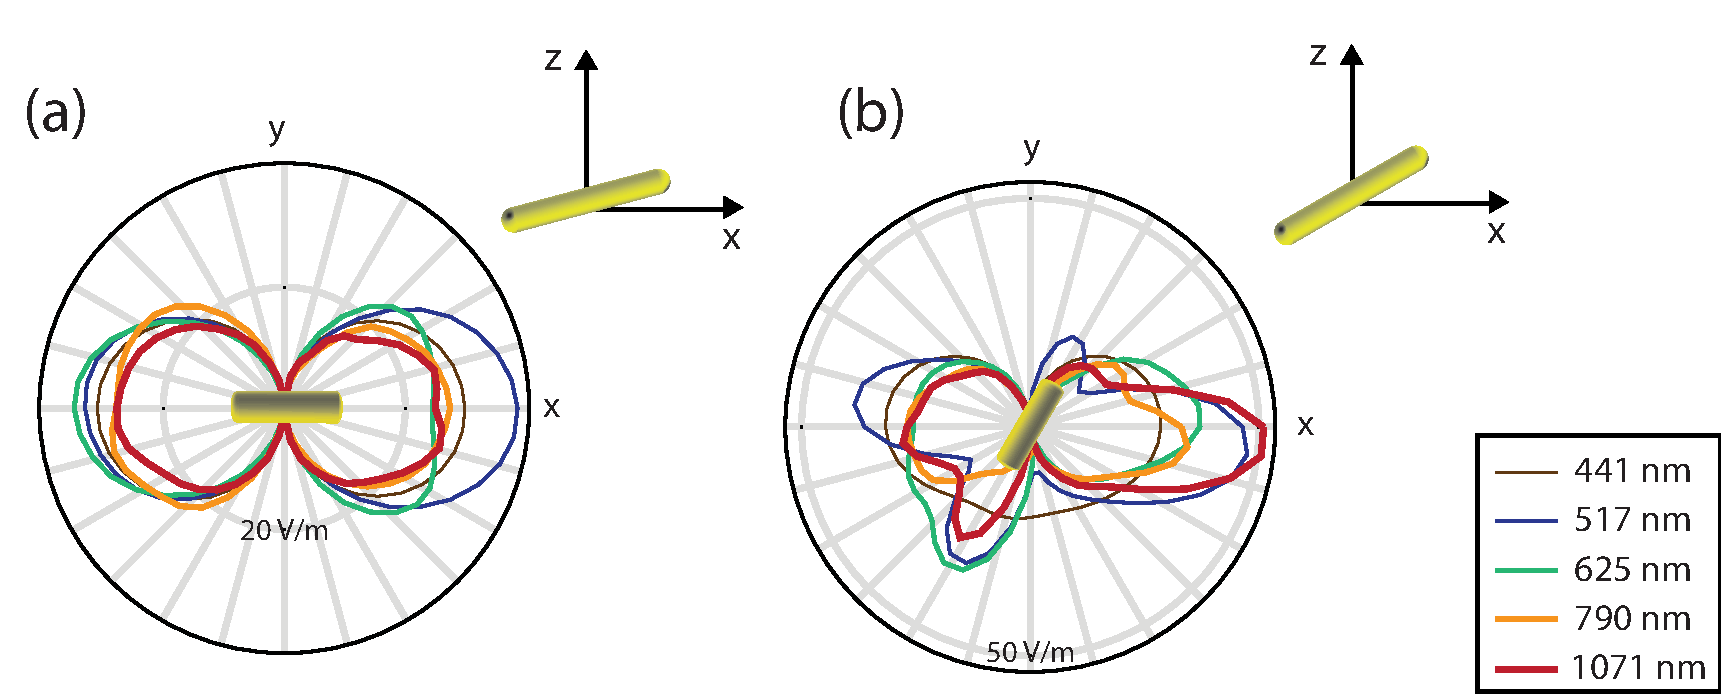
\includegraphics[width = 1.0\textwidth]{CPLComp.pdf}
\caption{Far-field radiation patterns for a nanowire aligned (a) in the $x$-$z$ plane with $\theta$ =75$^\circ, \phi$ = 0$^\circ$, (b) $\theta$ = 60$^\circ$, $\phi$ = 60$^\circ$ for wavelengths $\lambda$ = 441nm, 517nm, 625nm, 790nm, and 1071nm.}\label{CPLComp}
\end{figure}
\subsection{Momentum transfer via scattering}
It is expected that momentum transfer in the transverse $x$-$y$ plane associated with plasmons is observable in the scattered fields in order for linear momentum to be conserved and simulations indicate that momentum conservation is visible in the far-field power.
%The scattering of light is synonymous with the excitation of plasmons and thus a good indication of the plasmon dynamics.
Figure \ref{CPLComp} shows the electric field norm in the far field for two geometries to illustrate transverse forces, from which the scattering dynamics can be extrapolated. The momentum transfer to the nanowire can be inferred by the symmetry of the dipole  radiation patterns.  In Fig. \ref{CPLComp}(a), the nanowire is aligned in the $x$-$z$ plane with $\theta = 75^\circ$ and $\phi=0^\circ$.  At this orientation, the Lorentz force is calculated in the $x$-direction to be either negative ($\lambda =$ 441, 517nm) or positive ($\lambda =$ 625, 790, 1071nm) depending on the illuminating wavelength [Fig. \ref{FxFyFz}(a)].  A positive value of $F_x$, at a wavelength of $\lambda =$ 441nm is largely attributed to reflection since this wavelength is below the transverse-resonance cutoff.  At higher wavelengths, the $x$-direction shifts in the far-field radiated power correspond with the sign of the plasmonic Lorentz forces in the $x$-direction. The shape of the far-field radiation corresponds to the characteristic dipole radiation from excitation of the longitudinal TM$_0$ mode.

Similarly, in Fig. \ref{CPLComp}(b) shows a similar far-field normalized power for geometry $\theta$ = 60$^\circ$ and $\phi$ = 60$^\circ$.  Below the cutoff for plasmon excitation ($\lambda$ = 441nm), the radiation pattern indicates that momentum transfer in the $y$-direction is due to reflection. At higher wavelengths, an ``antenna'' behavior of the wire is apparent, the radiation pattern exhibits directionality.
% We observe that the wire radiates as an oscillating electric dipole in its transverse plane in addition to in the $y$-direction due to excitation of the transverse mode.
 The dipole radiation mode in the $y$-direction and transverse modes are uncoupled at $\lambda$ = 517nm, and the far-field radiation pattern is an `$x$' shape that is aligned with the axis of the nanowire. The size of the arms of the `$x$' shape determine the relative strengths of the dipole modes present, the arm perpendicular to the nanowire axis corresponds to the fundamental, TM$_0$ mode and the arm parallel to the HE$_{\pm1}$ modes.

At longer wavelengths the plasmonic Lorentz forces are significant [Fig. \ref{FxFyFz}]. For wavelengths and orientations that produce significant Lorentz forces the far-field radiation patterns differ greatly in symmetry from dipole radiation patterns one might expect. For wavelengths of $\lambda = 625, 790,$ and $1071$nm, the center of radiation pattern moves in the positive $x$ and negative $y$-direction, corresponding with $\mathbf{f}_M$ that is negative in the $x$ and positive in the $y$-directions [Fig. \ref{FxFyFz}].
%The scattering of light points to new self-action effects, which, in addition to reflection and radiation pressure, are observed in the far-field radiation power patterns.
Figure \ref{CPLComp} indicates that the plasmonically-induced Lorentz forces result in 50-70$\%$ changes in far-field radiated power, which is experimentally measurable.


\section{Torque in 3-dimensions}\label{3D}
\subsection{Torque visualized for various illumination wavelengths}
\begin{figure}[b]
\centering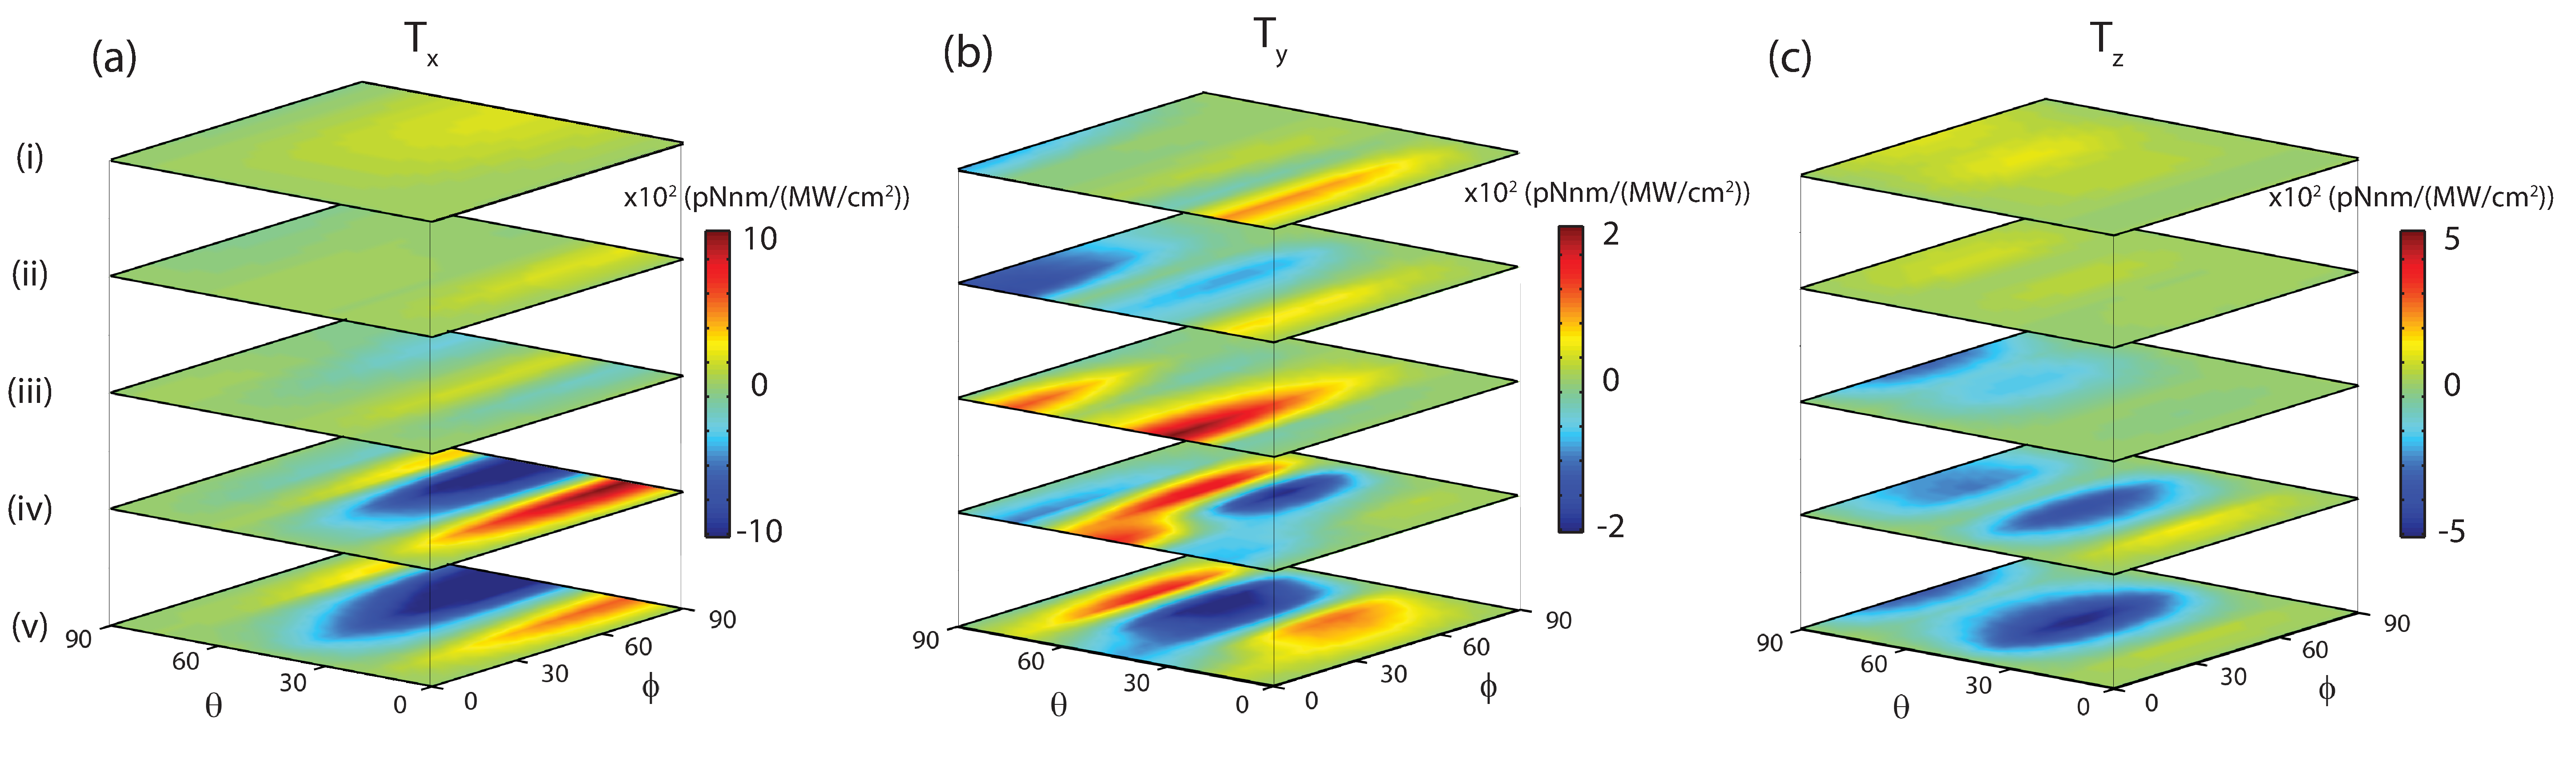
\includegraphics[width = \textwidth]{TNMT.pdf}
\caption{Torque around the (a) $x$-axis, (b) $y$-axis, and (c) $z$-axis at (i) 441nm, (ii) 535nm, (iii) 625nm, (iv) 790nm, and (v) 1071nm.}\label{TNW}
\end{figure}


The vector components of the dipole moment and plasmonically-induced Lorentz torque [$\mathbf{T}_E +\mathbf{T}_M = (T_x,T_y,T_z)$] are shown in Fig. \ref{TNW} for five wavelengths (441, 517, 625, 790, and 1071nm as chosen in the previous section).  Large values of $T_x$ and $T_z$ represent large torques that rotate the nanowire in both the polar and azimuthal directions. $T_x$ and $T_z$ increase in magnitude as wavelength increases which correlates well to the existence of chiral hybrid modes at longer wavelengths. Subsequently, whether $T_x$ and $T_y$ are positive or negative depends on the polar orientation of the nanowire.

The orientations that produce large net translation forces [Fig. \ref{FxFyFz}] do not necessarily coincide with large torques [Fig. \ref{TNW}]; the greater the asymmetry in $\mathbf{f}_E$ and $\mathbf{f}_M$, the greater the torque. Maximal torques produced by plasmons ($\mathbf{T}_M$) are an order of magnitude larger than the maximal torques produced by dipole moments ($\mathbf{T}_E$). Moreover, the magnitude of $\mathbf{T}_E$ is negligible at wavelengths above 600nm; above 600nm, $\mathbf{T}_M$ dominates. The magnitude of the $\mathbf{T}_E$ is the same sign in our hemisphere quadrant of $\theta$ and $\phi$ since $\mathbf{f}_E$ uniformly aligns the induced dipole with the axis of field polarization. In contrast, $\mathbf{T}_M$ changes sign with nanowire orientation and illuminating wavelength [Fig.~\ref{TNW}], which reflects the sensitive nature of the chiral hybrid plasmon.

\subsection{Phase diagram illustrations}
When the nanowire is free to rotate in three dimensions, the rotational behavior becomes complicated. The torque on the nanowire causes rotation which subsequently changes the torque on the nanowire. The results of this system that only accounts for Lorentz forces yields nonlinear dynamics that are beyond the scope of this chapter; nonetheless, the dynamics are illustrated with a phase portrait of the torques in spherical coordinates. The rotation in the $\theta$ and $\phi$ directions associated with $\mathbf{T}_E$  + $\mathbf{T}_M$ are:
\begin{eqnarray}
A_{\theta} &=& -\sin\phi T_x + \cos\phi T_y \label{Atheta}
\\A_\phi &=& T_z. \label{Aphi}
\end{eqnarray}

\begin{figure}[!ht]
\centering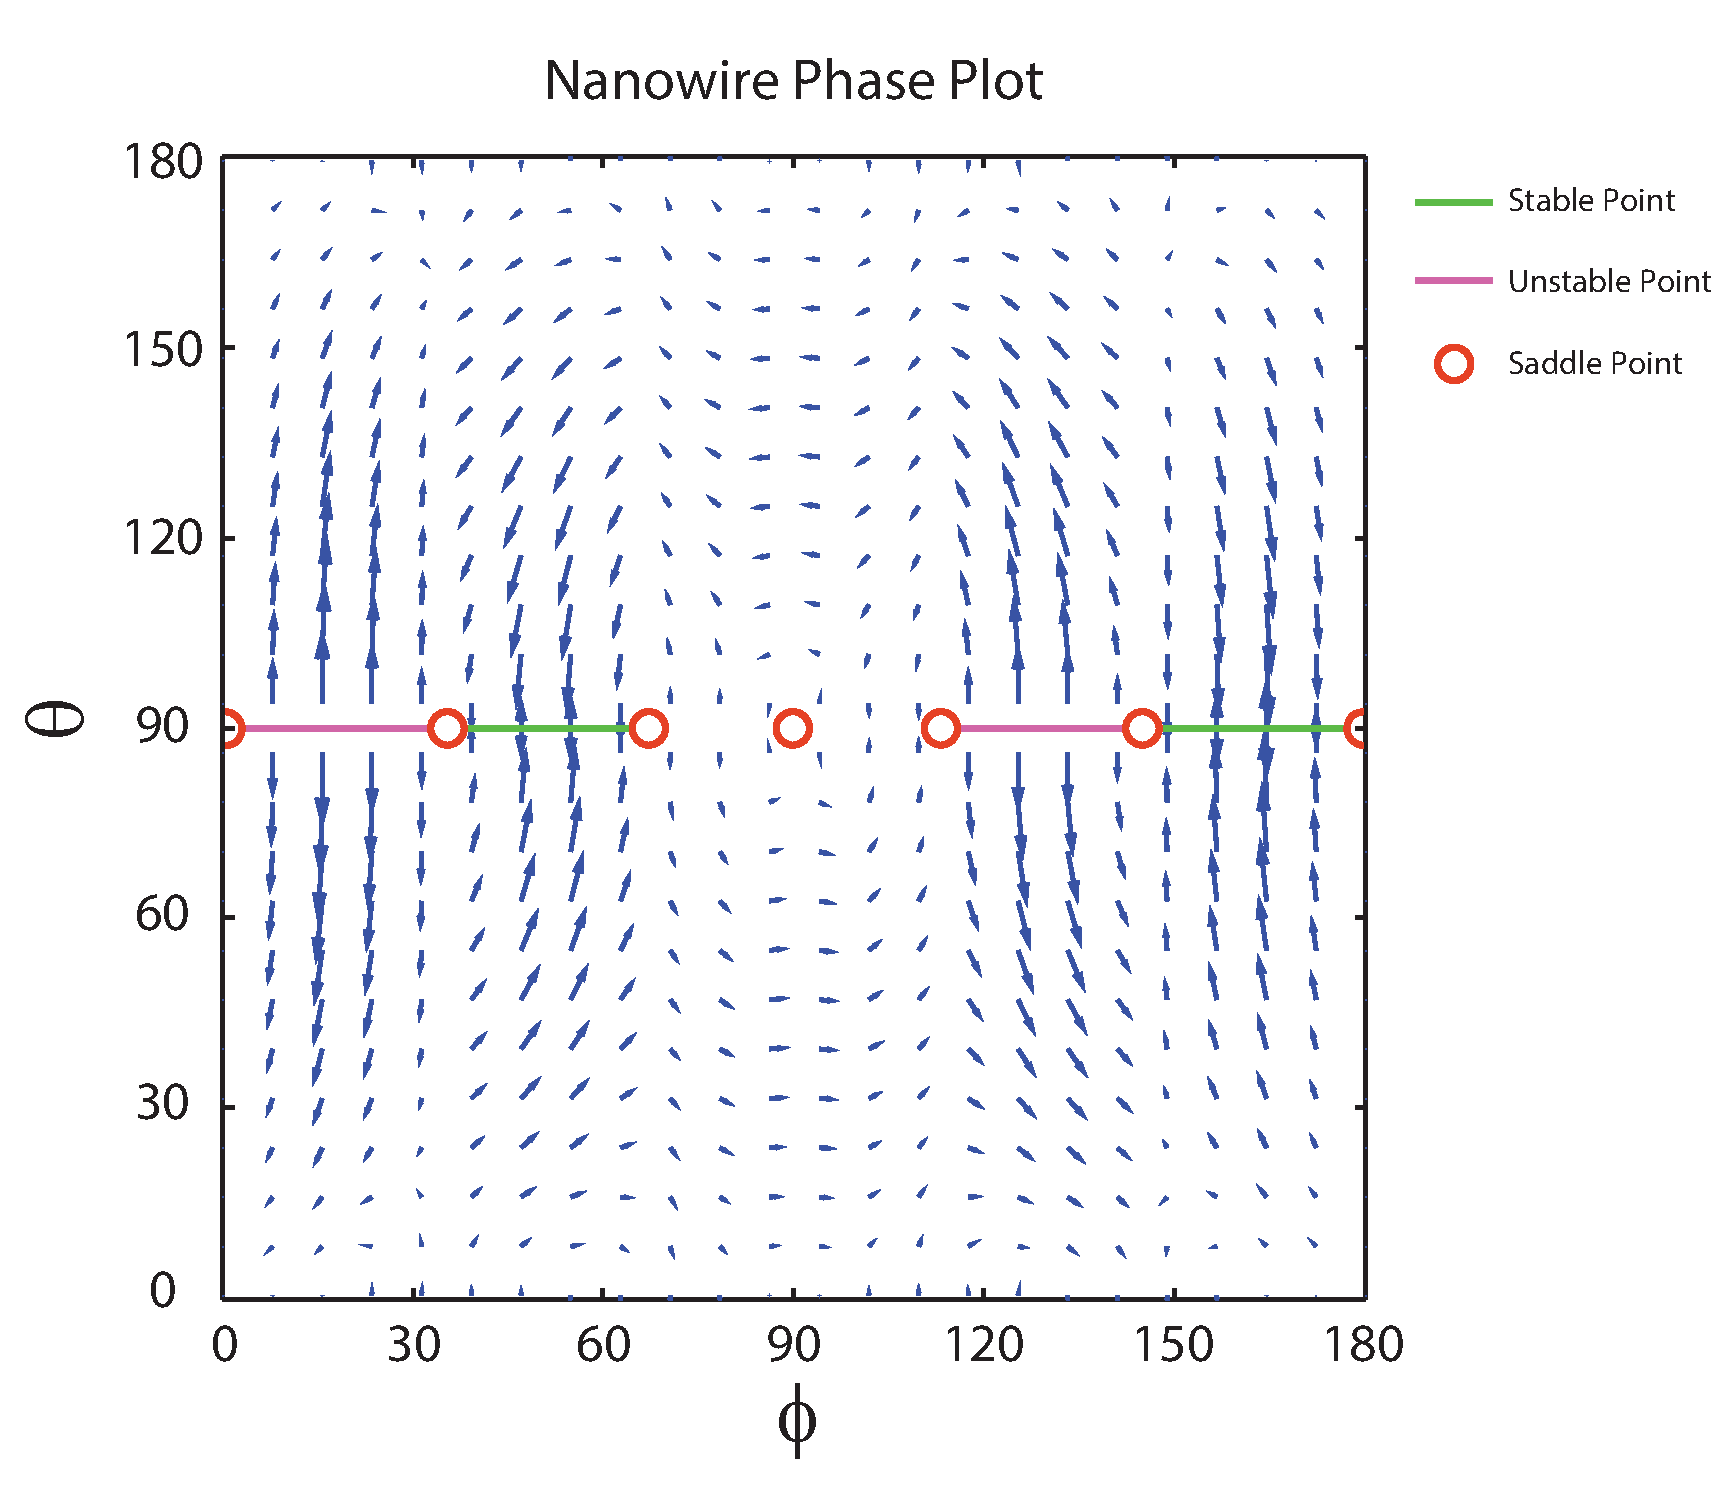
\includegraphics[width = \textwidth]{Rotational_Torque_1071nm.pdf}
\caption{Phase portrait of the torque forces calculated at $\lambda$ = 1071nm. Arrows in the $x$ and $y$ directions indicate torque that rotates the nanowire in the $\phi$ and $\theta$ directions respectively.}\label{RotTorq1071}
\end{figure}
The phase portrait, i.e. vectors $[A_{\phi},A_{\theta}]$ as a function of $\theta$, $\phi$ of the nanowire are plot in Fig. \ref{RotTorq1071}.
$A_{\theta}$ and $A_{\phi}$ are not equivalent to the angular acceleration since the rotational inertia, which changes as a function of angle, has not been taken into consideration. Moreover, the angular velocity will also influence the angular acceleration when the rotational inertia changes. Nonetheless, an understanding is gathered of the nanowire's stable orientations and dynamics from Fig. \ref{RotTorq1071}.

Points of stability occur when the angular motion is zero, which occurs when the torque is zero. Stable points occur when the vector field flows toward the point of zero torque; unstable points occur when the vector field flows away from the point of zero torque [\cite{Strogatz}]. Saddle points occur when the vector field flows toward the point of zero torque in one direction, and away in another.


Similar to the observation of the 2D nanowire dynamics [Sec. \ref{intro}], the nanowire aligns either parallel or perpendicular to the axis of polarization in a 3D system, settling at a stable point. Stable points occur when either $\theta$ or $\phi$ are equal to 0$^\circ$ or 180$^\circ$, and $\theta$ = 90$^\circ$ consistent with the strong orientational trapping observed in previous research [\cite{Yan2012a,Tong}]. Interestingly, along the line of $\theta$ = 90$^\circ$ stable, unstable and saddle points exist and illustrate many rich and complicated dynamics already reported with the optical trapping of nanowires. Around stable fixed points oscillatory dynamics occur: the nanowire will rotate, but more specifically, it will rock and spin in an oscillatory manner. Fig. \ref{RotTorq1071} also explains the rotational accelerations and rapid reversals seen in light-driven experiments [\cite{Shelton2005}] that are associated with the saddle point behavior and sharp inflections, such as those dynamics indicated at $\theta$ = 90$^\circ$.

This alludes to competing dynamics between the induced electric dipole and surface plasmons and explains the prior experimental observations that often contradict. It has been previously reported that nanowires align parallel or perpendicular to the linearly polarization of an optical trap. A theoretical model that limits consideration to $\mathbf{T}_E$ only explains the stable alignment of the dipole parallel to the polarization. Yet moreover, prior experiments employ trapping wavelengths in the near-IR [\cite{Tong}], where the magnitude of $\mathbf{T}_E$ is predicted to be negligible. This model predicts and explains the stable orientations of the nanowire, with longitudinal axis both parallel and perpendicular to the field polarization.

\section{Conclusion} \label{conclusion}
This chapter has shown that plasmonically-induced Lorentz forces are significant and greater than dipole-moment-induced forces, particularly at long-wavelength excitation between plasmon resonances.  The nanowire forces produced by plasmons lead to axial compression, which changes spatially along the nanowire surface depending on the nanowire orientation.  The existence of chiral plasmons coincides with spiral magnetic-field patterns that produce net transverse forces and torques, which is predicted to be experimentally observable in the far-field radiated power and polarization.  The plasmonically-induced Lorentz forces are expected to interfere with the optical trapping of nanowires; selection of a laser-trap wavelength that prevents the excitation of the chiral plasmonic modes will enable greater control over the optical manipulation of nanowires.

The rotational dynamics present a highly nonlinear and complicated problem due to the sensitive nature of the plasmonic resonance that conventional ray optics cannot explain. The plasmonically-induced Lorentz forces and torques produce rotational motion consistent with the spinning, rocking, and rapid reversals in rotation observed experimentally with elongated plasmonic nanoparticles.  Plasmonically-induced torque may oppose the dipole-induced torque, although the Lorentz torque dominates almost completely above the transverse resonance of the nanowire. This theoretical investigation is the first to properly explain the stable positions of nanowires under illumination of linearly-polarized electromagnetic fields, and reveals a rich system of optomechanical plasmonically driven dynamics that has not yet been explored.

This work also points to novel methods that manipulate conducting nanoparticles that do not result in the extreme absorption and heating generally associated with the excitation of plasmons; strong plasmonically-induced Lorentz forces occur off-resonance where plasmonic absorption is minimal. This outcome is highly relevant to the development of new devices and mechanisms that efficiently leverage the nonlinear mechanical dynamics of conducting nanoparticles in fluids, not limited to elongated conducting particles but also chiral nanoparticles, polymer materials, and carbon metastructures.

\section{Future work}
Future work on this subject may involve experimental verification of the theoretical and numerical components of the work shown here. An experiment may consist of an microscope setup with two tightly focused beams at different wavelengths. One beam would act as the optical trapping beam that would stabilize the nanowire at the focal point of the microscope setup similar to the setups described in the references [\cite{Ashkin2001, Lee2012, Kuo2001, Lang2003}], and the other would act as the excitation beam that would generate the Lorentz forces described in this chapter.
\clearpage

% chapter four
\chapter{Robustness and spatial multiplexing via diffractal architectures}
\chaptermark{Spatial multiplexing via diffractal architectures}
\section{Introduction}
Many natural systems exhibit fractal properties [\cite{Mandlebrot}]; in fact, scale invariance underlies many self-similar phenomena, from frost crystallization to animal colouration to stock-market pricing. In the realm of optics, the fractal anatomy of systems is widely associated with aggregated dielectric and metal colloids [\cite{Sorensen}], crystals [\cite{Macke}], and tissues [\cite{Schmitt}]. Fractal systems are also observed in nonlinear optics [\cite{Soljacic, Segev}] and fractalized optical properties can even efficiently characterize or enhance the response of materials [\cite{Stockman, Tsai}]. Less well utilized are the features of diffractals, or the diffraction patterns of fractal signals  [\cite{Berry,Horvath,Hou}]. Diffractals feature in methods of encrypting data [\cite{Barrera}] as a versatile approach to double random-phase encoding [\cite{Unnikrishnan}]. However, to differentiate from previous work fractal architecture is exploited to improve transmission robustness.

This chapter explores diffractals for their application in signal processing [\cite{Verma,Verma2}]. Free-space propagation of diffractal-signal architectures provides algorithmic value and spatial multiplexing properties; any arbitrary subsection of a diffractal contains sufficient information to recreate the original sparse signal that is transmitted with a specific fractal architecture. In a manner similar to compressive imaging [\cite{Kelly07, Howland}]\textemdash where sparse signals reveal greater information via the diffraction through structures\textemdash here the fractal structuring within the signal sparseness prevents the loss of information.

Like other applications of fractals in communications applications, the diffractal architecture exhibits trade-offs. Fractal antennas for the radio frequency and microwave regimes are known for being compact and versatile over wide spectral bands but are power intensive [\cite{Radonic,Puente-Baliarda}]; fractal encoding algorithms enable image compression with higher-resolution at the expense of greater algorithmic complexity [\cite{Jacquin}]; this chapter identifies that diffractal architectures prevent the loss of information but require greater signal preprocessing.  This investigation extends the understanding of fractal structures in signal communications and may increase robustness and transmission rates of satellite, wireless, and interplanetary communication systems, {\it i.e.,} networks that support a large number of roaming receivers.

%We analytically, numerically and experimentally show that a fractal structure on a sparse digital signal provides spatial multiplexing and robustness, as well as facile retrieval of the original sparse digital signal. 
The remainder of this chapter is organized as follows.  First, the form of a transmitted fractal signal is formalized, it is shown that the far-field diffraction pattern or diffractal is also a fractal, and the reciprocal nature of fractals is illustrated with the Sierpinski carpet. Second, the robust retrieval of a signal from a diffractal is demonstrated; the original signal is reconstructed even when the majority of the diffractal signal is blocked. Finally, the future applications for diffractal spatial multiplexing in free-space communication systems is discussed. 

\section{Theoretical description}\label{theory} 
\subsection{Spatial multiplexing of the diffractal} 

The fractal transmittance pattern is generated from any base matrix via recursive iterations where the matrix is resized and convolved with itself repeatedly [\cite{Allouche}].  The base matrix $B(x,y)$ adopts a general form,
\begin{equation}
B_i(x,y) = \sum_j\delta(xr^{i-1}-x_j,yr^{i-1}-y_j),
\label{BJ1}
\end{equation}
where the subscript denotes the iteration $i$, $r>1$ is the relative scaling between iterations, and $\delta(x-x_j,y-y_j)$ is the Dirac delta function at $x = x_j$ and $y=y_j$. 
The fractal transmittance function $T(x,y)$ is calculated recursively,
\begin{equation}
T_n(x,y) = T_{n-1}(x,y)*B_{n-1}(x,y),
\label{nTrans}
\end{equation}
where the subscript denotes the order of the fractal or its expression at the $n^{th}$ iteration, $T_0$ is the initial profile of 1's, and $*$ denotes the convolution operator.  

Subsequently, the diffractal is the Fourier transform or the far-field of the transmittance function $\tilde{T}$ [\cite{Horvath}],
\begin{equation}
\tilde{T}_n(k_x,k_y) = \tilde{T}_0(k_x,k_y)\prod_{i=1}^{n}\tilde{B}_i(k_x,k_y)\label{FTn}.
\end{equation}
The Sierpinski carpet is one example of a fractal that is generated by this process and via the iterated substitution of a $3\times 3$ base matrix of ones with removal of the center element:
\begin{equation}
\Bigg\{0\rightarrow \Bigg[\begin{array}{ccc}
0 & 0 & 0 \\
0 & 0 & 0\\
0 & 0 & 0\end{array}\Bigg], 1\rightarrow\Bigg[\begin{array}{ccc}
1 & 1 & 1 \\
1 & 0 & 1\\
1 & 1 & 1\end{array}\Bigg] \Bigg\}.
\label{baseMatrix}
\end{equation}

The second substitution of Eq.~\ref{baseMatrix} represents the mathematical expression for the base matrix $B_0(x,y)$.  In the case of the Sierpinski-carpet base-matrix elements, $r=3$, and $x_j$ and $y_j$ are the perimeter coordinates of a $3\times 3$ 9-unit block centered at the origin, and $(x_j,y_j)\in [(1,1),(1,0),(1,-1),(0,-1),(-1,-1),(-1,0),(-1,1),(0,1)]$. Since each of the Dirac delta functions in $B_0(x,y)$ yields a phase shift in the Fourier domain, {\it i.e.,} $\mathscr{F}\left\{\delta(\alpha x-x_i)\right\} = e^{2\pi i_ck_xx_i}/|\alpha|$, its scaled Fourier Transform at the $i^{th}$ iteration of the Sierpinski carpet [Eq.~\ref{BJ1}] becomes:
%\begin{equation}
%\tilde{T}_n(k_x,k_y) = \tilde{T}_{n-1}(k_x,k_y) r^{n-1}[4\cos(4\pi^2 3^{2(n-1)}k_xk_y)+2\cos(2\pi 3^{n-1}k_x)+2\cos(2\pi 3^{n-1}k_y)]
%\end{equation}
%The amplitude at each iteration is:
\begin{equation}
\tilde{B}_i(k_x,k_y) = (2/r)^{i-1}[\cos(2\pi3^{1-i}k_x)\cos(2\pi3^{1-i}k_y)+\cos(2\pi 3^{1-i}k_x)+\cos(2\pi 3^{1-i}k_y)].\label{BF}
\end{equation}
With each iteration, the spatial frequency components $k_x,k_y$ of the diffractal increase by a factor of 3 and spread the diffractal across a 3-times wider $k_x,k_y$-range, which is evident in Eq. \ref{BF}; the cutoff of $\tilde{T}_n$ scales in proportion with $k_x, k_y \propto r^{n-1}$. 

The Sierpinski carpet, $T$, is calculated recursively [Eq. \ref{nTrans}]: a second-order fractal is generated from the Kronecker tensor product of the base matrix $\Big[\begin{smallmatrix} 1 & 1 & 1 \\ 1 & 0 & 1\\ 1 & 1 & 1\end{smallmatrix}\Big]$ with itself; a third-order fractal is generated from the Kronecker tensor product of a second-order fractal and the same base matrix [see Appendix, \cite{Code1}]. Sierpinski carpets of $n= 1, 3,$ and $5$ are shown in Fig. \ref{AnalRecon}(a) with the corresponding diffractals $\tilde{T}$ [Fig. \ref{AnalRecon}(b)]. 

%\lstset{language = Matlab}
%\begin{lstlisting}
%function carpetHolo = Sierpinski(fracOrder);
%	carpetBase = ones(3); % Initialize matrix
%	carpetBase(2,2) = 0;
%	% Zero middle element
%	if fracOrder==0;
%		% For zero order case
%		carpetHolo = carpetBase;
%	else
%		% For higher order cases
%		carpetHolo= kron(carpetBase,carpetBase);
%		% For loop iterates the Kronecker tensor product
%		for i = 1:fracOrder-1
%			carpetHolo = kron(carpetHolo,carpetBase);
%		end
%	end
%end
%\end{lstlisting}

As the fractal order increases, $\tilde{T}$ exhibits smaller self-similar features at higher $k_x,k_y$;  the diffractal also exhibits a fractal architecture, as observed in other literature [\cite{Berry,Horvath}].  Moreover, when $n$ is large, an arbitrary subsection of $\tilde{T}$ closely resembles the whole, and the self-similarity is already apparent with $n= 5$ [Fig. \ref{AnalRecon}(c-d)]. The iterated, self-similar, wide-spatial-frequency features contained in the diffractal $\tilde{T}_n$ [Eq. \ref{FTn}] enable robust reconstruction of itself, which is described in the next subsection.

\begin{figure}[t!]
 \includegraphics[width=\textwidth]{AnalyticalHolgramReconstruction.pdf}
\caption{(a) Signal patterns, or fractalized signals (FS) of orders $n = 1$, $3$, and $5$. (b) Corresponding Fourier transforms of signals on logarithm scale, or diffractal signals (DS). (c) Reconstructed Fourier-transforms (RFS) from the 1\% black-outlined subset, the blocked diffractal signal (BDS). (d) Enlargement of a portion of the $n=5$ diffractal, which illustrates similar patterns at different length scales.}
\label{AnalRecon}
\end{figure}

\subsection{Robust reconstruction of a blocked diffractal signal} 

The sparse matrix $B_0$ and transmitted signal $T$ are referred to as the original and fractalized signal, OS and FS, respectively; the diffractal signal DS is $\tilde{T}$, or, the Fourier transform of FS; BDS refers to an off-axis subsection of DS that is filtered; a reconstructed fractalized signal RFS refers to the inverse-Fourier transform of BDS; a regenerated version of the original signal ROS interpolates RFS in order to obtain OS.  

In Fig.~\ref{AnalRecon}(b), a subsection or BDS is outlined with a black square, which represents 1\% of DS. The corresponding RFS from BDS are shown in Fig. \ref{AnalRecon}(c). For $n$ = 1, 3, RFS is ostensibly blank because BDS carries negligible power.  In contrast, when $n=$ 5, RFS carries features that resemble FS. The capacity to reproduce FS with 1\% of the off-axis area from DS is referred to as ${\it robust}$ reconstruction.  

Robust reconstruction\textemdash where RFS resembles FS\textemdash is possible even when the size of BDS is significantly reduced [\cite{Verma}].  A corresponding increase in the FS fractal order $n$ will yield RFS that resembles FS when BDS is arbitrarily small. With the example of the Sierpinski carpet, Fig. \ref{AnalRecon}(a)--\ref{AnalRecon}(c), if the size of BDS is reduced to 1\% of OS, then a comparable RFS is produced by increasing the fractal order of FS from $n=1$ to $n = 5$. 

Robust reconstruction is defined as the capacity to regenerate OS from RFS from a simple threshold function [see Appendix, \cite{Code2}]. The threshold function of the Sierpinski carpet divides RFS into a $3\times 3$ array (identical size as OS) and measures the intensity in each of the 9 elements. Above a certain threshold value, the element is assigned a value of 1, and otherwise assigned a value of 0. The $3\times 3$ array that is processed with the threshold function, ROS, is theoretically identical to OS when OS is transmitted with the diffractal architecture. 

%\begin{lstlisting}
%function recon = reconFun(Threshold,carpetBaseLength,carpetHolo)
%	% Ratio of length of hologram
%	normLength = length(carpetHolo)/carpetBaseLength; 
%	
%	% Convert to array of cells
%	cellHolo = mat2cell(carpetHolo,repmat(normLength,1,...
%	carpetBaseLength),repmat(normLength,1,carpetBaseLength));
%	
%	% Calculate mean, determine if above threshold value, and plot
%	pcolor(double(cell2mat(cellfun(@mean2, cellHolo))>Threshold));
%end
%\end{lstlisting}

The comparison between RFS and FS in peak signal-to-noise ratio (PSNR) for various fractal orders as a function of the fractional BDS size is shown in Fig.~\ref{PSNR}. The error bars represent the standard deviation from the mean value of 200 random locations of BDS. Since the size of RFS is reduced from FS, RFS is resized with nearest-neighbour interpolation. 2 observations from Fig.~\ref{PSNR} are provided: first, when BDS is greater than 0.01\% of the fractional size of FS, larger fractal orders produce higher PSNR; second, as the fractional area of BDS increases the location of BDS becomes irrelevant since the standard deviation around the mean diminishes. For fractional BDS sizes smaller than 0.01\% lower fractal orders yield a higher PSNR since the minimum size matrix needed to completely recreate FS is larger for higher fractal orders. For example the minimum size matrix needed to recreate FS of order 1 is $3\times 3$, for FS of order 2 it is $9\times 9$, etc. 

\begin{figure}[t!]
\begin{centering}
 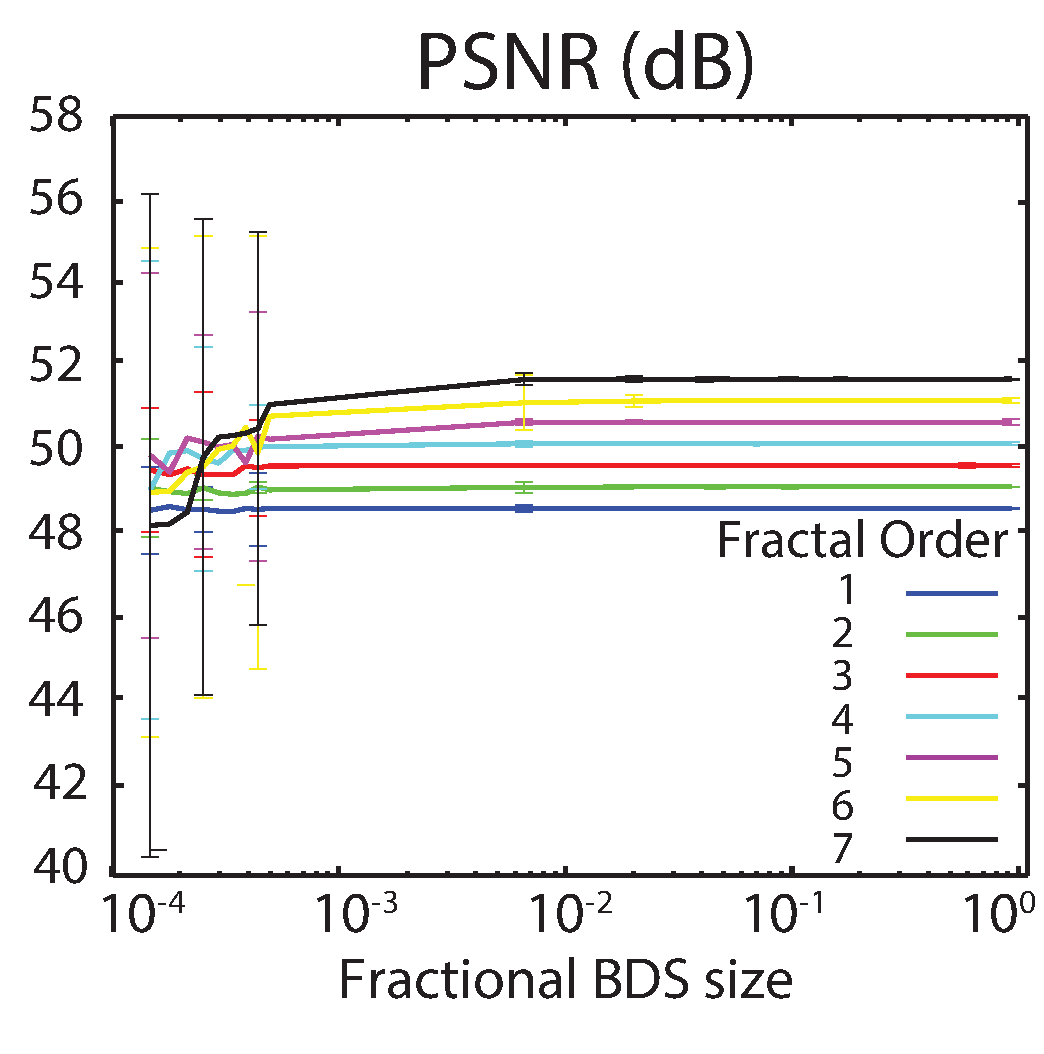
\includegraphics[width=0.7\textwidth]{psnr_good_eb2.pdf}
\caption{The peak signal-to-noise ratio (PSNR) of RFS to FS for various fractal orders as a function of the fractional BDS size.}
\label{PSNR}
\end{centering}
\end{figure}

ROS is generally identical to OS when BDS is above 0.01\% and the fractal order is greater than 3, regardless of BDS location. A partial explanation for the robust reconstruction is that increasing-order FS carry arbitrarily-high $k_x,k_y$ and enable arbitrarily-{\it small} BDS to carry the information of FS or OS.  If OS is strictly limited to binary or Dirac-delta functions, then FS has no $k_x,k_y$ cut-off and as $n$ approaches infinity, fractalized features appear in FS without a $k_x,k_y$ cut-off.  In fact, the amplitude of the additional $k_x,k_y$ gained from each iteration scales inversely with $r^{n-1}$, which provides a detection limit only in practice; in theory, each iteration generates high-$k_x,k_y$ copies of OS [Eq.~\ref{baseMatrix}] that are spatially distributed from the origin.  

Yet it is worth noting that the robust reconstruction is achieved because the diffractal architecture also couples $k_x$ and $k_y$ in iterated products [Eq.~\ref{FTn}].  As a result, RFS will resemble FS when either the BDS size {\it or location} changes.  In a manner similar to spatial filtering, RFS will produce outlines of FS if $n$ is not sufficiently large; however, unlike a high-pass spatial filter of a multi-scale random high-$k_x,k_y$ pattern [\cite{Kelly07}], a change in the location or the size of BDS will not distort the outline of RFS.  Subsequently, the diffractal architecture provides superior performance over other algorithms that regenerate sparse data, OS [\cite{Kelly07, Howland}].   


%\begin{equation}
%H = \frac{1}{2m}(p_x^2 + p_y^2) + \frac{1}{2} M{\Omega}^2
%     (x^2 + y^2) + \omega (x p_y - y p_x).
%\end{equation}

\section{Experimental results} \label{experiment}
\indent The features of diffractals are experimentally demonstrated with a 4-$f$ optical arrangement where the 2-dimensional Fourier transform of a collimated fractal image, DS, lies in the focal plane of an imaging lens \cite{Goodman}.  The experimental setup that produces, filters and reconstructs FS is shown in Fig. \ref{ExpSetup}(a) and experimentally reconstructed images, RFS, are shown in Fig. \ref{ExpSetup}(b). An aperture of area approximately $0.8mm^2$ blocks the majority of DS. The placement of the aperture is shifted roughly $4mm$ horizontally and $5mm$ vertically from the central point, in the focal plane of the lens. The SLM image has a resolution of 800$\times$600 pixels (16mm$\times$12mm).  

\begin{figure}[t!]
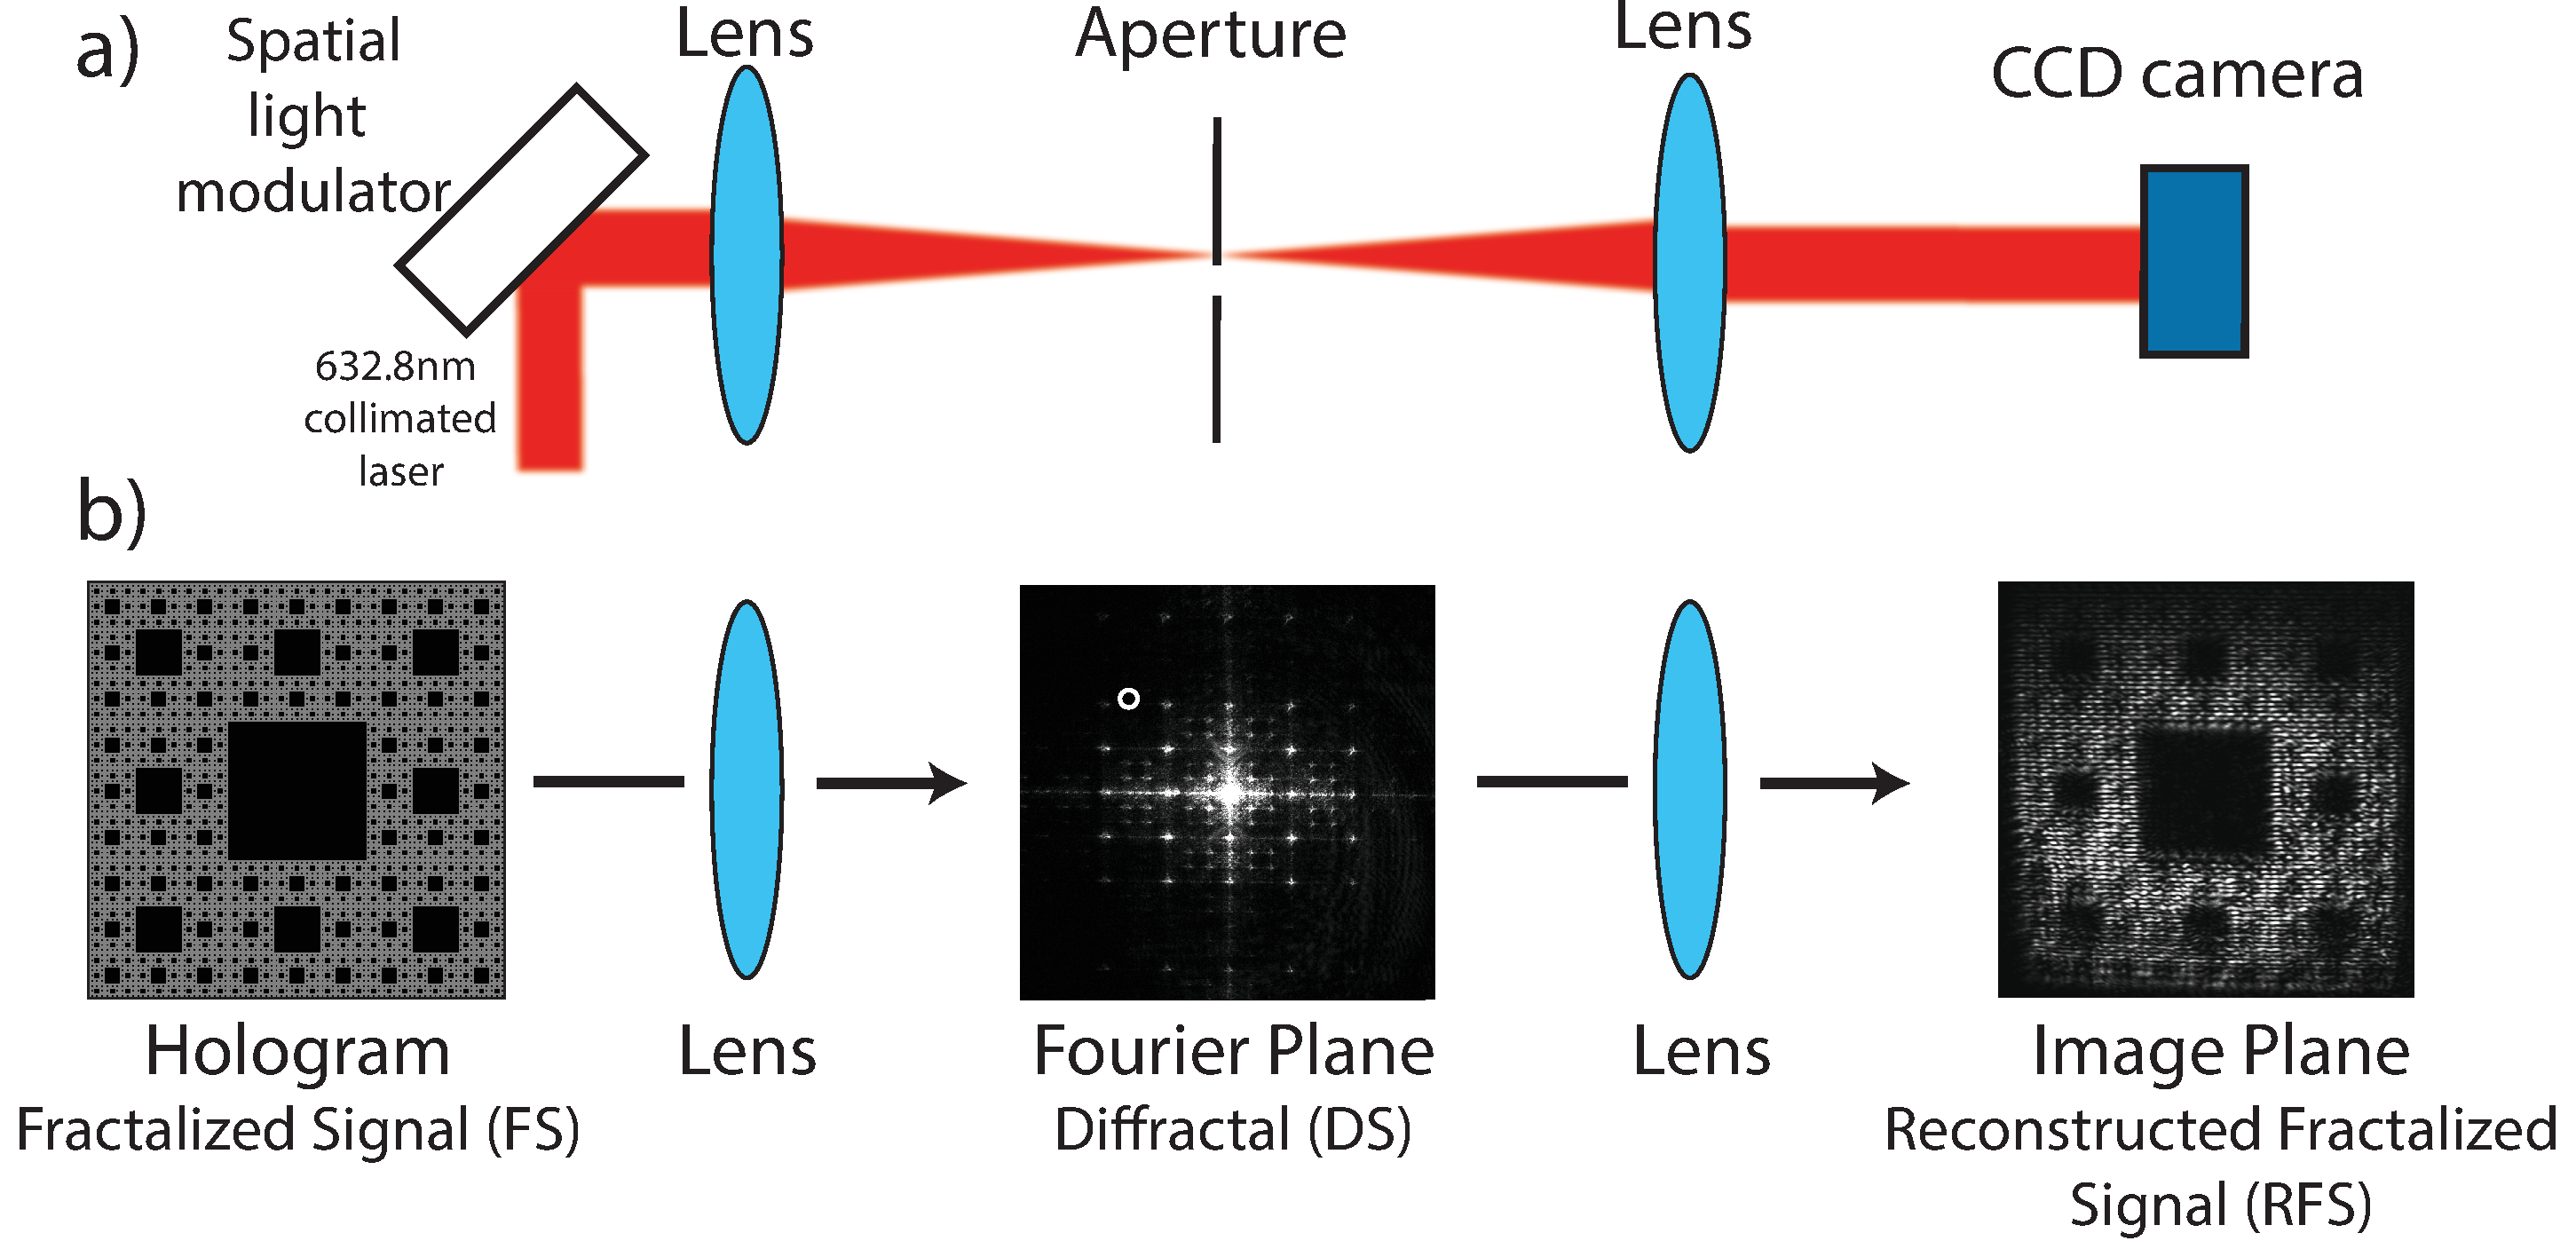
\includegraphics[width=\textwidth]{ExpMethod.pdf}
\caption{(a) Light from a $\lambda = $ 632.8-$nm$ wavelength laser is spatially filtered, expanded, and collimated and illuminates the full area of a 800x600 pixel spatial light modulator (SLM). The 4-$f$ system is composed of 2 5-$cm$ lenses placed after the SLM. The first lens Fourier transforms the fractal signal (FS) at the focal plane. An aperture is placed off-center at the focal plane and only transmits a portion of the diffractal (BDS). The second lens reconstructs the SLM image with the light that is transmitted through the aperture. (b) The Sierpinski carpet hologram of order $n$= 5, CCD image in the focal plane of the hologram after the lens, and the reconstructed image. A circle denotes the area utilized to reconstruct the image.}
\label{ExpSetup}
\end{figure}

When high order diffractal architectures are employed ($n>$4), a phenomenon is observed that is shown numerically: the placement of the aperture in DS is irrelevant in order to reconstruct the original image. When the aperture is moved laterally in the focal plane, RFS maintains strong resemblance to FS. In fact, only the intensity of RFS diminishes as the aperture translates further from the DS center; the outline remains fixed as the aperture moves.  For smaller fractal orders, RFS resembles FS only when the aperture is placed within $0.8mm$ of the center, where the spatial frequency components are concentrated. The signal-to-noise of the experiment and CCD camera sensitivity limit effective reconstruction, while the highest order $n$ is of FS is limited by the number of SLM pixels.  

\section{Discussion of applications}\label{disc}
A distinction is made that diffractals are specific fractal structures. Not all fractals enable robust signal communications and the recursive transformation employed to generate FS and DS in Eq.~\ref{BJ1} and~\ref{BF} differ fundamentally. For example, both of the Fourier Transform pairs FS and DS are fractals and carry iterated, self-similar features, but if the roles were reversed in the transmission system, the reconstruction will instead depend severely on the size and location of BDS. In fact, if in the example of the Sierpinski carpet, the center subsection becomes BDS, then the ROS will not resemble the OS, regardless of fractal order.  The diffractal is unique from general fractals and self-similar scale-invariance alone is an insufficient precondition for our system of robust reconstruction and spatial multiplexing. 

It may seem contradictory that higher-order fractals lead to more robust signal transmission since the finer structure of a higher-order fractal is itself harder to reconstruct. There are two perspectives of diffractals that explain the robust reconstruction. First, the self-similar structures of higher-order fractals have a greater spatial frequency range and finer detail, and subsequently smaller BDS carry sufficient information to reconstruct OS. Second, the higher-order diffractals carry higher spatial-frequency components where the $k_x$ and $k_y$ components are coupled, and subsequently the location of the subsection in DS is unimportant. In these experiments BDS of arbitrary size and location carry sufficient information to reconstruct OS but in practice, there exists clear limitations for the robust reconstruction even in the limit of infinite-order FS.  

Note: it may also seem contradictory that an infinitesimally-sized BDS with infinitesimal power can carry information-- this is not actually true: there is a minimal size for BDS fixed by the pixelation of the SLM.
There exists a trade-off with the diffractal architecture between robust reconstruction and high bit rate; a greater bit-rate is achieved with a larger base matrix, which can limit the maximum fractal order that is transmitted.  For example, with the $3\times 3$ or 9-element OS, there are 512 possible spatial bits, three of which are illustrated in Fig. \ref{Multiplex}(a-c).  A $4\times 4$ base matrix requires $(\frac{4}{3})^{2n}$ more pixels than a $3\times 3$ to achieve the same fractal order, $n$. With a limited SLM pixel resolution, there is a choice between the generation of higher-order fractals and the utility of higher spatial bits.   

If the trade-off between bit-rate and robust reconstruction are mitigated, then the diffractal architecture could support a large number of roaming receivers with only one transmitter, such as wireless or satellite networks shown in Fig. \ref{Multiplex}(d). The self-similar properties of the diffractal architecture and their corresponding far-field pattern provide a method to reach a large number of receivers, possibly moving, without signal degradation.  The processing times required in the calculation of FS from OS are not trivial and scale with $r^{2n}$. Furthermore, the refresh rates of a spatial light modulator or similar adaptive-optics device present constraints on the maximum achieved bit rate, which requires further consideration.  

\begin{figure}[t!]
\includegraphics[width=\textwidth]{Multiplexing2.pdf}
\caption[]{Three examples of 512 9-bit spatial patterns, associated with base matrices 
(a) $\Big[\begin{smallmatrix} 1 & 0 & 1\\ 1 & 1 & 1\\ 1 & 0 & 1 \end{smallmatrix}\Big]$, (b) $\Big[\begin{smallmatrix} 1 & 1 & 0 \\ 0 & 1 & 1\\ 0 & 1 & 1\end{smallmatrix}\Big]$, and (c) $\Big[\begin{smallmatrix} 1 & 0 & 0 \\ 1 & 1 & 0\\ 1 & 1 & 1\end{smallmatrix}\Big]$. The fractal signals FS are shown with their corresponding experimentally-reconstructed fractal signals RFS from the experimental setup in Fig. \ref{ExpSetup}(a).  The lower-right inset shows the reconstructed original signal ROS. (d) Example application: transmitted fractal signal FS is received at a far-field distance as a diffractal signal DS, where a roaming set of receivers, with only a diffractal subsection BDS, reconstructs the original signal OS.}
\label{Multiplex}
\end{figure}
This can be applied to more complex shapes and structures, for example, an $16\times 16$ pixel smiley face shown in Fig.~\ref{face}. The Fourier transform of the smiley face is taken; part of the Fourier transform is blocked; and a reconstruction of the image is attempted via the inverse Fourier transform. The same experimental procedure as shown in Fig.~\ref{ExpSetup} is utilized. As can be seen from Fig.~\ref{face} when just the image is sent through the experimental setup the image reconstructed is not recognizable at all. However when the image is fractalized even just one order the image becomes recognizable. Unfortunately due to the limitations of pixels on the SLM no higher orders can be achieved.\\
\begin{figure}[h!]
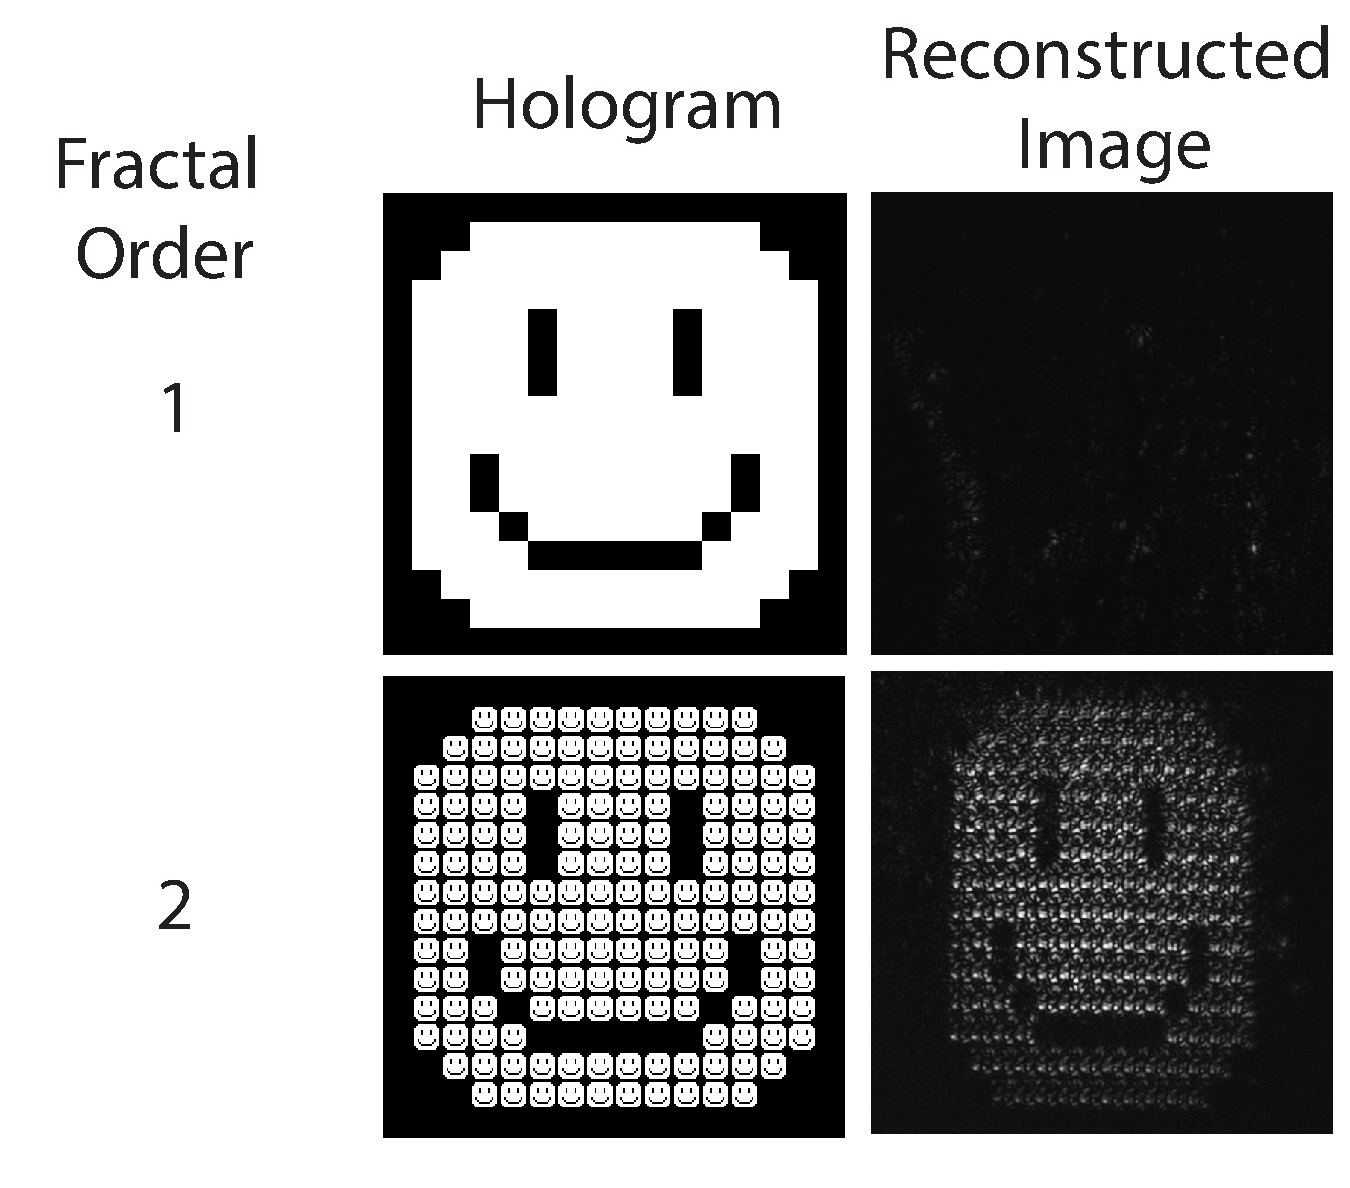
\includegraphics[width=\textwidth]{imgRecon.pdf}
\caption[]{As an example of a more complicated image, a smiley face is fractalized, the Fourier transform is taken, 99\% of the signal is blocked at the focal plane, and the image is reconstructed. This is compared to the original signal that is not fractalized.}
\label{face}
\end{figure}

Fractal structures have been utilized in signal communications and data compression for decades. Fractal antennas for the radio frequency and microwave regimes are known for being compact and versatile over wide spectral bands [\cite{Radonic,Puente-Baliarda}]. Fractal encoding algorithms enable image compressing with higher-resolution compression at the expense of greater algorithmic complexity [\cite{Jacquin}]. The trade-off for higher resolution fractal-compressed images is higher processing times, which presents a limitation of their presence in data communications. Recently, however, there has been a resurgence of interest in fractal architecture due to their robust properties in optical transmission.

\section{Conclusion}
This chapter has shown that the diffractal architecture provides the beneficial features of spatial multiplexing and robust reconstruction. Demonstrations have been shown with the Sierpinski carpet, a familiar fractal, although the results could have been demonstrated with 511 other patterns similarly imprinted with the diffractal architecture. Data that is transmitted with the diffractal architecture is highly robust to intermediate-obstacle signal blocks and diffractal subsections of arbitrary size and location carry sufficient information to regenerate the original signal without distorting outlines of its pattern.  This research illuminates potential applications in data transmission systems when one transmitter sends data to a large number of moving receivers or through noisy media.

\section{Experimental difficulties and future work}
A SLM works well for experimentation because of its facile reconfigurability, however the resolution is limited to 800$\times$ 600 pixels, that limits the complexity of the data image sent in the process. Ways to overcome this could be to use photolithography to create transmission structures with a larger pattern on a glass film, however the structure would lose the reconfigurability that the SLM possesses. Transmission could even be created by printing the transmission structure pattern on transparency sheets, which would be a cheap alternative method to achieve similar results with a lower resolution.
\clearpage

% chapter five
\chapter{Meta-optical chirality and emergent eigen-polarization modes via plasmon interactions}
\chaptermark{Meta-Optical Chirality}
\def\rcurs{{\mbox{$\resizebox{.16in}{.08in}{\includegraphics{ScriptR}}$}}} 

\section{Introduction} 
Metamaterials are composed of sub-wavelength components, or meta-atoms that individually alter the intensity and phase of light. When placed on a 2D surface, metamaterials are known as metasurfaces [\cite{Zhao}] and have enabled many applications from quarter [\cite{Yu}], half-wave plates[\cite{Ding}], and cross-polarizers [\cite{Qin}], to ultra-thin lenses [\cite{Aieta,Ni}]. Chiral metasurfaces can ultimately be defined as those that exhibit a response dependent on the incident circular-polarization handedness, though the specific mechanism behind the phenomena has been debated; it has been argued that planar structures such as metasurfaces cannot exhibit true optical activity (OA) or circular dichroism (CD) without the excitation of magnetic resonances since certain 3D symmetry properties are not satisfied [\cite{Hentschel, Eftekhari}]. The equivalent response from planar metasurfaces can be achieved by alternate methods such as the interaction of plasmon modes [\cite{Eftekhari, Fan10}], or by non-radiative dissipation [\cite{Khanikaev}], and is named optical chirality. The difference in transmission from different polarization states due to optical chirality produces an \textit{equivalent} effect to OA and CD. 	

Optical chirality in metamaterials is produced in several ways. Not surprisingly, a chiral metamaterial can be composed of chiral meta-atoms, in which the mirror image of the structure cannot be superimposed on the original [\cite{Zhang:14, Tang2016}]. Intrinsically chiral materials are chiral due to the geometry of the meta-atoms themselves, and exhibit chiral behavior at normal illumination incidence. Helices [\cite{Kuzyk}], gammadions [\cite{Cao13, Kwon08}], or nanoparticle assemblies [\cite{FanSci, Guerrero-Martinez}] are common examples of intrinsically chiral meta-atoms that exhibit a strong chiral response. Another approach that achieves chiral asymmetry is the creation of a linear phase gradient, {\it i.e.}, illumination at oblique incidence [\cite{Yannopapas,Cao, Cao15, Cao15_2, Proscia}] or spatial variation of the unit cell [\cite{Aieta, Yu,Shaltout}]. The chiral response that arises from the linear phase gradient of either of these approaches is associated with extrinsic chirality.  

This chapter instead focuses on the optical chirality that arises solely from the interactions between achiral meta-atoms. It is postulated that the nonlinear coupling between meta-atoms originates from an interaction force derived from the Li\'{e}nard-Wiechert potential [\cite{jackson}], which accurately predicts measured changes in the experimental transmission spectra.  Rectangular plasmonic resonators are studied whose arrangement leads to chiral phenomena at normal incidence, or identical tilted achiral nanostructures in a lattice that lead to a chiral response. The individual nanostructures are achiral, yet the periodic array is chiral [\cite{Plum11, Prosvirnin}], and thus any chiral response distills the interaction between plasmonic structures. Optical chirality is expected when the lines of mirror symmetry of the nanostructures do not coincide with the lattice array \textemdash the mirror image cannot be superimposed with the original. ``Meta-optical chirality" refers to the macroscopic optical chirality that is both observed in the far-field and attributed to the interactions between plasmonic resonators.  While many have alluded to the coupling between meta-atoms [\cite{Hentschel, Hentschel:10, Metzger, Na, Rozin}], few have addressed the origin of the interaction force.  
 
Experimentally, a simple Babinet-inverted rod (dimensions $\approx \lambda/5$) is employed as the meta-atom of the metasurface and arranged in a square array. When rod-shaped nanoapertures are tilted at an angle of $22.5^\circ$ and illuminated with low-intensity visible light ($\ll 1W/cm^2$), CD is measured on the order of 0.6 degrees of ellipticity.  In comparison, while optimized and twisted split ring resonators can reach CD up to 16 degrees in the near infrared [\cite{Decker}], such meta-atoms require small features ($\approx \lambda/20$). The relatively-large dimensions of the rod nanoapertures support dipolar plasmon resonances and can be fabricated easily with robust large-area processes. An approach is demonstrated here that leverages the interactions between simpler meta-atoms in order to achieve an optical chirality.  The general approach boasts facile design, circumvents the complex structures that intrinsically chiral materials generally require, and forgoes the oblique illumination angle-of-incidence that is the crux of extrinsically chiral materials.

The chiral response exhibited by this metasurface design is both appreciable and unexpected since plasmonic interactions generally manifest as nonlinear optical responses, which require high illumination intensities [\cite{Metzger2, Kauranen}]; optical chirality are observed at intensities far below those generally required to yield nonlinear optical responses. The metasurface is interrogated with a continuum of polarization states and find that the metasurface cannot be characterized simply from its response from orthogonal circular-polarization modes.  In fact, a conventional transmission matrix description of the polarization properties is insufficient to accurately describe the optical behavior of the metasurface.  An alternative analytic representation is provided and supports a description of intensity-independent, weakly-nonlinear plasmonic limit cycles.  The model also explains why the emergence of multiple eigen-polarization modes is observed, which is also measured experimentally. The work presented in this chapter furthers the understanding of metasurface design and breaks from the long-standing convention of transmission matrices.

\begin{figure}[b!]
\centering
\includegraphics[width=\linewidth]{springs_image11.eps}
\caption{(a) Model representation: an array of plasmonic resonators (rod-shaped apertures) tilted at $\theta_s$ relative to the base of the unit meta-atom the resonators are separated into $m$- and $n$-type. The interaction force on $m$-type resonators results from the 4 nearest $n$-type resonators and vice-versa. (b) The interaction Lorentz force that arises from Larmor radiation [Eq.~\ref{eq:Fint}] for various $\theta_s$ when resonators oscillate in the $x$-direction, as a function of time. (c) The interaction force in the parallel ($x$), and perpendicular ($y$) directions when the resonators oscillate in the $x$-direction, as a function of $\theta_s$.}
\label{fig:model}
\end{figure}
 
\section{The coupling force}
In this model, the interaction between neighboring plasmonic resonators is defined as the Lorentz force produced from the oscillation of adjacent resonators. The interaction force is derived from the electromagnetic field of an accelerating charged particle given by the Li\'{e}nard-Wiechert potential [\cite{jackson}]. The force from an $m^{th}$ charge on the $n^{th}$, $\vec{F}^{int}_{mn}$, is:   
\begin{eqnarray}
 \vec{F}^{int}_{mn} = k_eq_nq_m\bigg(\frac{\hat{\rcurs}_{mn}-\vec{\beta}_n}{(1-\vec{\beta}_n\cdot\hat{\rcurs}_{mn})^3R_{mn}^2}\bigg) + \frac{k_eq_nq_m}{c}\bigg( \frac{\hat{\rcurs}_{mn}\times[(\hat{\rcurs}_{mn}-\vec{\beta}_n)\times\dot{\vec{\beta}}_n]}{(1-\vec{\beta}_n\cdot\hat{\rcurs}_{mn})^3R_{mn}}\bigg)
 \label{eq:Fint}
\end{eqnarray}
where $k_e$ is Coulomb's constant $=1/4\pi\epsilon_0$, $\epsilon_0$ is the permittivity of free space, $\vec{\beta}_{n} = \dot{\vec{r}}_n/c$, $c$ is the speed of light, $\hat{\rcurs}_{mn} = \frac{\vec{r}_m - \vec{r}_n}{|\vec{r}_m - \vec{r}_n|}$ is the unit direction from the $m^{th}$ charge to the $n^{th}$, $R_{mn}$ is the lattice distance, $q_n$ is the charge of the $n^{th}$ particle, and $\vec{r}_m, \vec{r}_n$ are the positions of the $m^{th}$, and $n^{th}$ resonator, respectively, from the origin. When the charges are stationary, Eq.~\ref{eq:Fint} collapses to the Coulomb force between two charged particles. The first term of Eq.~\ref{eq:Fint} is referred to as the ``velocity field" since it is independent of acceleration, and the second term is the ``acceleration field". With motion of the charges restricted to the 2-D plane of the metasurface, the interaction forces created by the surrounding resonators are produced in the plane of the metasurface. Though charges also oscillate in the $z$-direction, an investigation into the coupled behavior of the longitudinal fields is beyond the scope of this study. The associated Lorentz forces may explain the near-to-far-field coupling [\cite{Vuong}].

A representation of the model is shown in Fig.~\ref{fig:model}(a), in which all nanostructures are tilted by $\theta_s$ relative to the base of the unit cell. The tilt effectively restricts the direction of motion of the resonator and the interaction force is incorporated into the equations of motion for a Lorentz-Drude plasmonic resonator [\cite{Rakic}]. The metasurface is modelled such that there is no spatial variation of the unit cell, \textit{i.e.}, all nanoapertures are tilted at the angle, $\theta_s$. For analytical reasons the $x$ and $y$-axes also rotate by $\theta_s$ such that the long (short)-axis of the plasmonic resonator is always parallel with the $x$ ($y$)-axis. The $\theta_s$ determines the directions of $\vec{\beta}_m$, and $\vec{\rcurs}_{mn}$ in Eq.~\ref{eq:Fint}.
The resonators are placed in a checkerboard-like pattern of $m$- and $n$-type oscillations, and calculate the motion of each set of resonators. The second-order terms cancel by symmetry, and subsequently the interaction force between resonators scales inversely with the distance cubed. The four closest resonators provide the interaction force that couple motion in the $x$- and $y$-directions, and between $m$- and $n$-type resonators. Interaction forces from diagonal dipoles are between like-type resonators ($m$-$m$, $n$-$n$) and are neglected, in part because the increased distance between resonators reduces the interaction force, and also because the focus is on the interactions between $m$- and $n$-type. %The inclusion of interaction force from further dipoles would reduce the . 

%The interaction force [Eq.\ref{eq:Fint}] is illustrated as a function of time for various sample angles in Fig.~\ref{fig:model}(b), and as a function of sample angles, $\theta_s$, in (c), from Eq.~\ref{eq:Fint} where .
 
The total interaction force from the Larmor radiation of the four closest resonators is shown in Fig.~\ref{fig:model}(b-c), where $\beta = -i\omega x_0/c\hat{i}$ and $x_0$ is the maximum displacement of the charge oscillation, and $x_0 = 20$nm. Each resonator oscillates in the $x$-direction and produces a force in both parallel ($x$) and perpendicular ($y$) directions, $F_{\parallel}$ and  $F_{\perp}$. $F_{\parallel}$ is calculated to be approximately 20 times larger than $F_{\perp}$.
The $F_{\parallel}$ \textemdash which is always co-aligned with the long axis of the nanostructures\textemdash is maximal when the nanostructures are oriented at 0$^\circ$ or 90$^\circ$ with the edge of the unit cell. $F_{\parallel}$ couples the parallel motion between adjacent resonators in the formation of hybrid modes, which is documented in the subsequent section. When the angle of the nanostructure, $\theta_s$, is 0$^\circ$, 45$^\circ$, or 90$^\circ$, $F_\perp$ is zero, as shown in Fig.~\ref{fig:model}(b-c). These angles correspond to the lines of symmetry of the square lattice; the array is not intrinsically chiral. Alternatively, the magnitude of $F_{\perp}$ is maximized at 22.5$^\circ$, and 67.5$^\circ$ which would correspond to opposite-handed chiral structures. $F_\perp$ couples to the orthogonal dipole moment of the adjacent resonators and is the source of optical chirality in the metasurface studied, which is further documented in the following section. Though this model incorporates the Li\'{e}nard-Wiechert potential from rectangular nanostructures, the model can be generalized to model the interaction forces from arbitrary plasmonic shapes and arrays.

If the array was non-chiral there exists some combination of reflection, rotation, and translation of the nanoaperture array can be superimposed on the original. Figure~\ref{fig:chiral} illustrates that when the nanoapertures are tilted at an angle $\theta_s \neq b\times 45^\circ$ the modified array cannot be superimposed with the original, where $b$ is some integer.
\begin{figure}[th!]
\centering
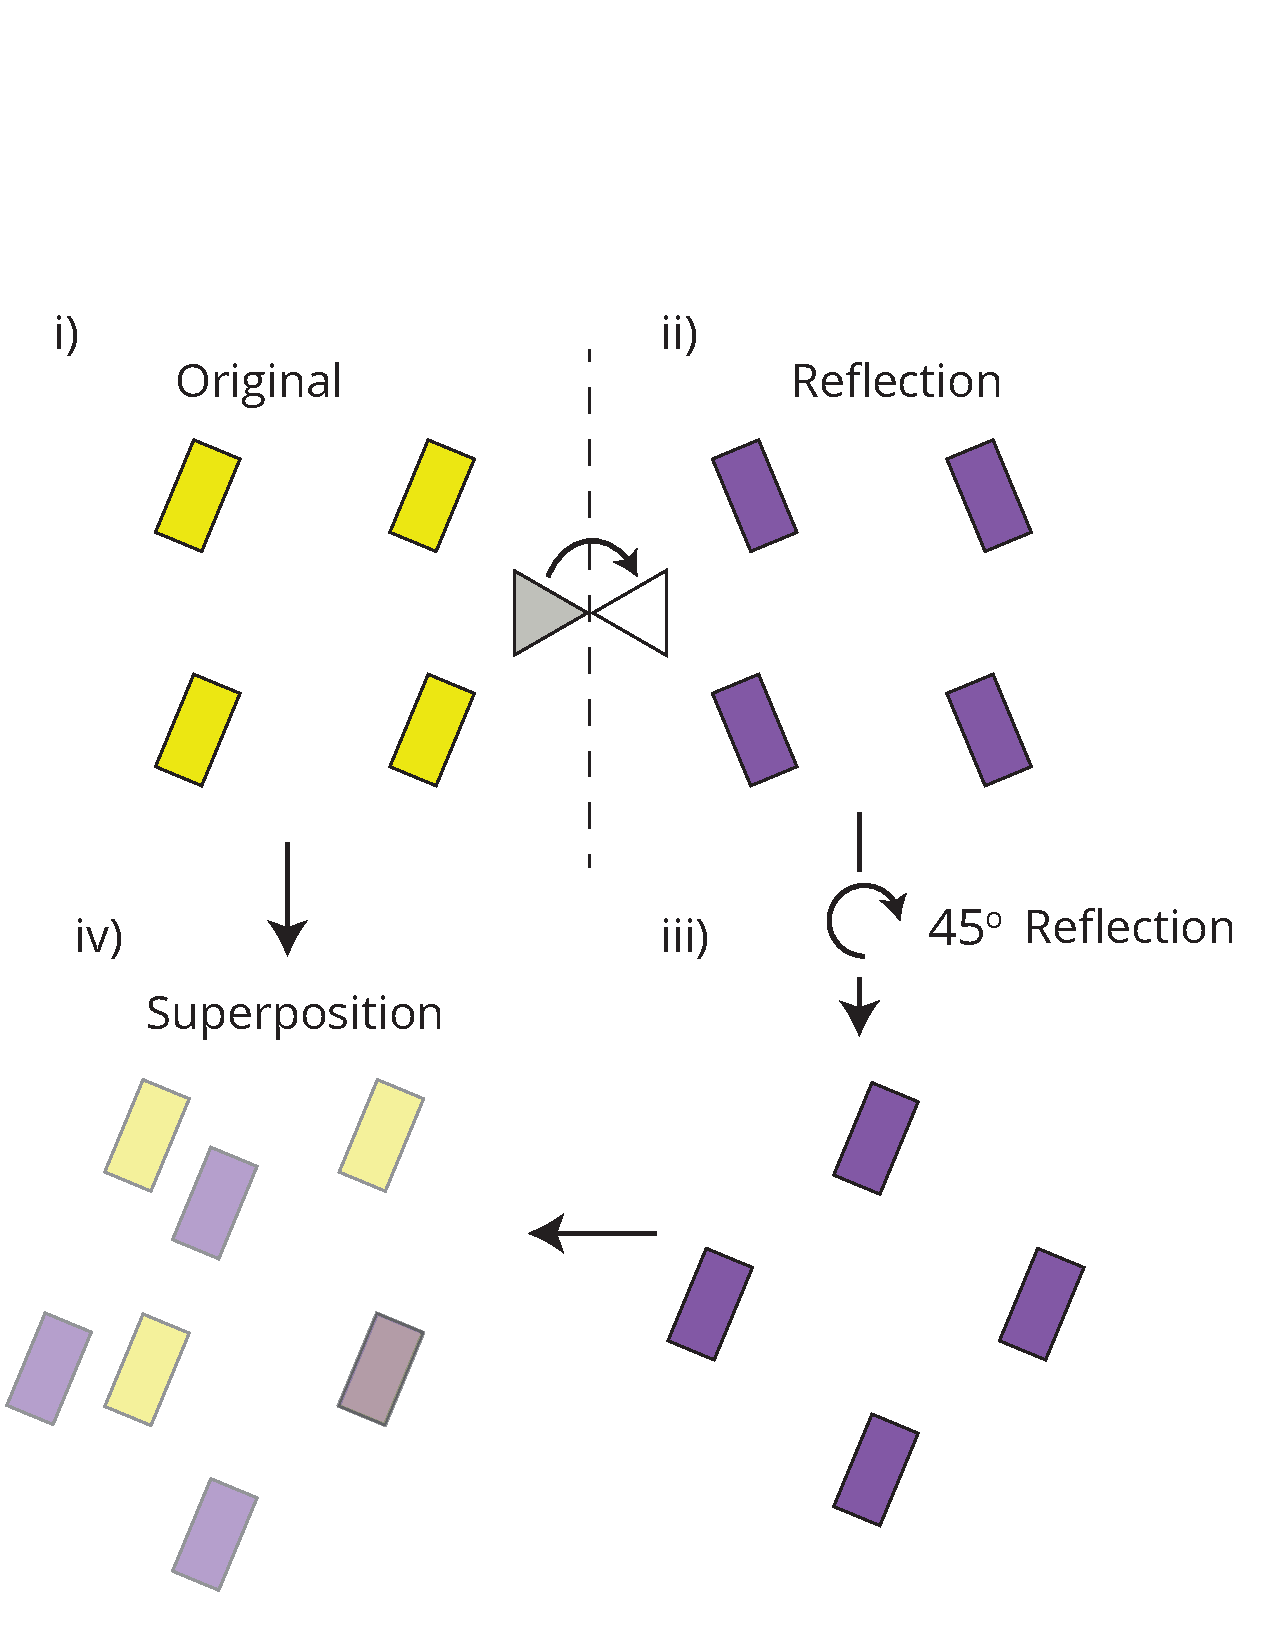
\includegraphics[width=0.9\linewidth]{chirality_proof.pdf}
\caption{(i) The original array with tilt angle, $\theta_s = 22.5^\circ$. (ii) Reflection along the vertical axis. (iii) Rotation by 45$^\circ$. (iv) Superposition of the original array with the modified array.}
\label{fig:chiral}
\end{figure}
\section{Coupled equations of motion}
The interaction force [Eq.~\ref{eq:Fint}] is summed from the four neighboring resonators to the Lorentz-Drude model and incorporate its interaction as a perturbation with the parameter, $\delta$:
$M\ddot{\vec{r}}_{m/n} = -M\omega_0^2\vec{r}_{m/n} -M\gamma\dot{\vec{r}}_{m/n}+q\vec{E}e^{-i\omega t} + \delta\sum_{n/m}  \vec{F}^{int}_{mn}$, where $r$ is the displacement of the resonator from its equilibrium position, $M$ is its mass, $\omega_0$ is the natural harmonic frequency of the resonator, $q$ is its charge, $\gamma$ is the velocity-dependent damping rate, $E_0$ is the strength of the incident driving electric field, with frequency $\omega$, subscript $m/n$ refers to the motion of either $m$- or $n$-type resonators, and dot formalism corresponds to derivatives with respect to time, $t$. 
 A separate solution is adopted for the displacement of the $m$- and $n$-type resonators shown below:
\begin{eqnarray}
x/y(t) = \frac{E_{x/y}q/M}{\omega_{0x/y}^2-i\gamma \omega-\omega^2}e^{-i\omega t} + \underbrace{x_{h}/y_{h}(t)}_\text{homogeneous solution}+ \underbrace{\delta x_{1}/\delta y_{1}(t)}_\text{perturbed solution},
\label{unperturbed_solution}
\end{eqnarray}
which includes a homogeneous solution, $x_h, y_h$, often neglected [\cite{Metzger,Metzger2,Rakic}].% An equivalent solution exists for $n$-type oscillators.
 The homogeneous solution is the general solution to the equations of motion in the absence of an external electric field and its solution is determined from the initial conditions. Even though the homogeneous solution is neglected in Optics texts [\cite{MaierBook, Levi:16, Raether:88}], it is generally present in studies of vibrations and when solving for the limit cycles of weakly nonlinear oscillators [\cite{Strogatz}]. No exact analytical solution exists for the system in which the interaction force is included; our quantitative perturbative approach employs a Taylor expansion of the interaction force, 
\begin{multline}
\vec{F}^{int}_{mn} \approx \frac{k_eq_nq_m}{R_{mn}}\Bigg[\frac{\big(\hat{\rcurs}_{mn}-\vec{\beta}_n\big)}{R_{mn}} +	 \Big(\hat{\rcurs}_{mn}\times[(\hat{\rcurs}_{mn}-\vec{\beta}_n)\times\dot{\vec{\beta}}_n]\Big)\frac{1}{c}\Bigg] \\ \times \bigg(1+3\vec{\beta}_n\cdot\hat{\rcurs}_{mn} -6(\vec{\beta}_n\cdot\hat{\rcurs}_{mn})^2-10(\vec{\beta}_n\cdot\hat{\rcurs}_{mn})^3\bigg)
 \label{eq:Fint_taylor}.
\end{multline}
%We approximate a linear relationship between the interaction force and electric field, however when the force is included into the equations of motion [Eq.~\ref{eq:Fint_taylor}], nonlinear limit cycles result.
The low-power case is considered where the transmitted polarization is independent of illumination intensity and the interaction force is linear with respect to the electric field. The system remains nonlinear because the optical response cannot be described by a superposition of incident fields. %Due to symmetry arguments, second-order electric-field terms cancel. The $\delta$ term of the perturbation analysis yields the equations of motion,
\begin{equation}
\begin{aligned}
\begin{bmatrix}\ddot{x}_{1,m}\\\ddot{y}_{1,m}\end{bmatrix} +\begin{bmatrix}
\omega_{0x}^2 & 0\\
0 & \omega_{0y}^2
\end{bmatrix} \begin{bmatrix}x_{1,m}\\y_{1,m}\end{bmatrix} +\gamma\begin{bmatrix}\dot{x}_{1,m}\\\dot{y}_{1,m}\end{bmatrix} =  \frac{1}{M}q_m\begin{bmatrix}
\kappa_{1x,n} & \kappa_{3x,n}\\
\kappa_{3y,n} & \kappa_{1y,n}
\end{bmatrix}\begin{bmatrix}E_x\\E_y\end{bmatrix},\\
\begin{bmatrix}\ddot{x}_{1,n}\\\ddot{y}_{1,n}\end{bmatrix} +\begin{bmatrix}
\omega_{0x}^2 & 0\\
0 & \omega_{0y}^2
\end{bmatrix}\begin{bmatrix}x_{1,n}\\y_{1,n}\end{bmatrix} +\gamma\begin{bmatrix}\dot{x}_{1,n}\\\dot{y}_{1,n}\end{bmatrix} =  \frac{1}{M} \underbrace{q_n\begin{bmatrix}
\kappa_{1x,m} & \kappa_{3x,m}\\
\kappa_{3y,m} & \kappa_{1y,m}
\end{bmatrix}\begin{bmatrix}E_x\\E_y\end{bmatrix}}_\text{$F^{int}$},
\label{eq:xymotion}
\end{aligned}
\end{equation}
where
\begin{multline}
\kappa_{1x} =  A_x\bigg[3k a + 2 i + 6+3k^2
\bigg(-  \langle x_{h}\rangle^2 (3ka\cos(4\theta_s)+A) \\ + \langle y_{h}\rangle^2 (9ka\cos(4\theta_s)+A)+\langle x_{h} y_{h}\rangle 9ka \sin(4\theta_s)\bigg)\bigg],
\end{multline}
\begin{multline}
\kappa_{1y} = A_y \bigg[3k a + 2 i + 6+3k^2
\bigg(  \langle y_{h}\rangle^2 (3ka\cos(4\theta_s)+A) \\ + \langle x_{h}\rangle^2 (9ka\cos(4\theta_s)+A)-\langle x_{h} y_{h}\rangle 9ka \sin(4\theta_s)\bigg)\bigg],
\end{multline}
\begin{equation}
\kappa_{3x} = 3A_xk^2
\bigg[ 3ka\sin(4\theta_s)(3\langle x_{h}\rangle^2 - \langle y_{h} \rangle^2)-3\langle x_{h} y_{h}\rangle(9ka\cos(4\theta_s)+A)\bigg],
\end{equation}
\begin{equation}
\kappa_{3y} = 3A_yk^2
\bigg[- 3ka\sin(4\theta_s)(3\langle y_{h}\rangle^2 - \langle x_{h} \rangle^2)-3\langle x_{h} y_{h}\rangle(9ka\cos(4\theta_s)+A)\bigg],
\label{kappas}
\end{equation}
and where $A_x = \frac{2k_eq_mq_nk}{Ma^2}g_{x}$, $A_y = \frac{2k_eq_mq_nk}{Ma^2}g_{y}$, $A=3ka+4i$, $a$ is the periodicity of the metasurface, $k$ is the incident wavevector, $\langle\rangle$ denotes the time-average, and $g_{x/y} =\frac{1}{\omega_{0x/y}^2-i\gamma\omega-\omega^2}$. 
 
While Eq.~\ref{eq:xymotion} may resemble a transmission-matrix formalism, the equations of motion of one type of resonator are coupled to the other by its homogeneous solution and subsequently, there are four coupled equations of motion instead of two. When the $m$-type resonators are excited, they generate Lorentz forces via the Li\'{e}nard-Wiechert potential, which contribute to both parallel and perpendicular motions of the $n$-type resonators.

The perpendicular Lorentz force couples to the orthogonal modes of the different resonators, which leads to optical chirality in the metasurface. In order to understand the terms of Eq.~\ref{kappas}, the plasmonic resonators are restricted to move only in either the $x$- or $y$-directions in the fundamental solution. The perturbative interaction becomes $\kappa_{3x/y} = \pm\frac{9k_eq_mq_n2k^4}{M a}g_{x/y}\langle y_{h}/x_{h} \rangle^2\sin(4\theta_s)$, which is zero when $\theta_s = 0^\circ, 45^\circ, 90^\circ$, \textit{etc.}, in agreement with the exact evaluation of $F^{int}$ [Fig.~\ref{fig:model}(b-c)]. Maximal optical chirality is achieved when the nanostructures are tilted at $\theta_s =$ 22.5$^\circ$ and 67.5$^\circ$. 

\begin{figure}[b!]
\centering
\includegraphics[width=\linewidth]{figure_439_wRoltLin13_wSEM.eps} 
\caption{(a) A top-view scanning electron microscope image of the metasurface. (b) The transmission spectra associated with different linear polarization angles, where the presence of bonding and anti-bonding modes is observed. (c) Shift in the wavelengths of the bonding and anti-bonding modes as a function of polarization angle. (d) Interaction forces parallel and perpendicular to the polarization axis experienced by the resonators from Eq.~\ref{eq:xymotion} as a function of polarization angle.} 
\label{fig:rotlin}
\end{figure}

\begin{figure}[b!]
\centering
\includegraphics[width=\linewidth]{exp-OR-CD_varyPol4.eps}
\caption{(a) The optical rotation (OR) and change in the elliptical component as a function of input polarization at 660nm. Inset: the relationship between $E_x$ and $E_y$ OR and change in the elliptical on the polarization ellipse. (b) OR and circular dichroism (CD) calculated from a transmission (T-)matrix approach (dashed). Overlaid is the experimental measurements of OR (measured at $\psi=$+30$^\circ$), and the CD (solid).} 
\label{fig:CD-OR}
\end{figure} 
\section{Mode hybridization and optical chirality}
Experimentally, a metasurface is fabricated that maximizes $F_\perp$ or $\kappa_{3x/y}$ with $\theta_s = 22.5^\circ$, % We show a scanning electron micrograph of the metasurface in Fig.~\ref{fig:model}(c) 
in which rod nanoapertures are arranged on a 30-nm gold film and measure 160nm by 80nm, as shown in Fig.~\ref{fig:rotlin}(a). The periodicity, $a$, varies the relative strength of the interaction force.
A periodicity of 375nm is employed in a square array, which is small enough to observe the coupling between nanoapertures, yet large enough so that the individual responses are still present.   

The wavelength-dependent transmission properties are explored in Fig.~\ref{fig:rotlin}(b), which shows the transmission for linearly-polarized light. The axis of the illuminating linear polarization is rotated counter-clockwise from 0$^\circ$ (vertical) through 90$^\circ$ (horizontal) to 180$^\circ$ (vertical). Two absorption dips are observed in the transmission around 600nm and 730nm that correspond to the mode-splitting or mode hybridization of the plasmonic dipolar resonance [\cite{Prodan}]. 
The spectral locations of the bonding and anti-bonding modes correspond to the mode coupling or interaction force $F^{int}$. When the periodicity decreases, $F^{int}$ increases and the resonances separate further; if the separation between meta-atoms increases, then the transmission resonances collapse to the transmission profile of a single resonator [\cite{Prodan}]. The trends associated with meta-atom spacing indicate that the transmission dips observed are not a Wood's anomaly grating effect, which is related to lattice absorption. Wood's anomaly resonances would scale in proportion with the metasurface spacing. Moreover, Wood's anomalies are characterized by ultrasharp resonances [\cite{Yang16}] which are not observed. 

The parallel component of the interaction force leads to the mode-splitting in the metasurface. The spectral difference between the bonding and anti-bonding modes is shown in Fig.~\ref{fig:rotlin}(c) with a Savitzky-Golay filter [\cite{Savgol}] overlaid. The interaction force is evaluated in the approximation [Eq. \ref{eq:xymotion}] in order to relate the model to the mode splitting. The components of the interaction force, $F_{\perp}$, $F_{\parallel}$, and $|F| = \sqrt{F_{\perp}^2+F_{\parallel}^2}$ are shown in Fig.~\ref{fig:rotlin}(d), where the input polarization is rotated from 0$^\circ$ to 180$^\circ$. The $F_{||}$ and the trendline of the spectral shift both exhibit maximal values between 45$^\circ$ and 55$^\circ$, where the illuminating linear polarization connects opposite ends of vertically-adjacent resonators.  The minimal values of the spectral splitting occur between 135$^\circ$ and 145$^\circ$ and correspond with an angle where the illuminating linear polarization connects opposite ends of horizontally-adjacent resonators.  Differences between the model and experiment result from the fact that in the model, only $20$nm resonator displacement is considered whereas in experiment, the effective resonator dipole is the length of the nanorod, or $180$nm. Moreover, the approximation of $F^{int}$ only accounts for the four nearest resonators and incorporates only time-harmonic terms.  Nevertheless, the strength of the parallel force $F_{||}$ scales approximately with the experimentally-measured spectral splitting of transmission resonances. 
 
The interaction force leads to other experimentally-measured polarization-dependent metasurface responses.  
The metasurface is illuminated with linearly-polarized light (ellipticity $\chi< 1 ^\circ$) at a wavelength $\lambda = 660$nm and observe that the transmitted changes in the azimuthal and elliptical components of the fields, $\Delta \psi$ and $\Delta \chi$, depend on the angle of linear polarization [Fig.~\ref{fig:CD-OR}(a)]. The change in azimuth $\Delta \psi$ denotes optical rotation (OR) and the change in the elliptical component $\Delta \chi$ denotes the phase accumulation between the $E_x$ and $E_y$-components. When the illuminating polarization angle rotates a full revolution, the trendline for the OR exhibits 4 inflection points. The OR and the perpendicular interaction force $F_\perp$ follow a similar trend [Fig.~\ref{fig:rotlin}(d)], which is expected since $F_\perp$ is the source of the optical chirality in our metasurface.  

Optical chirality is conventionally determined by the off-diagonal elements of transmission matrix of the metasurface  [\cite{Wu16, Plum14,Plum11}] but there are limits to this transmission matrix formalism. The polarization density of the material is calculated with the relation $\vec{P} = N_0q\vec{r}$, where $N_0$ is the free charge carrier concentration of the material, $q$ is the charge of the particles, and $\vec{r}$ is the direction and subsequently:
$\vec{P} = N_0q\begin{bmatrix}
x_0+x_1\\y_0+y_1
\end{bmatrix} = \epsilon_0(\epsilon-1)\vec{E}(\omega, r)+\Gamma(\nabla\times\vec{E}(\omega,r))$, and the non-locality parameter, $\Gamma_{x/y} = \frac{iN_0q_mq_n\kappa_{3x/y}}{k(\omega_{0x/y}^2-i\gamma\omega-\omega^2)}$, and $\Gamma$ is the mean of $\Gamma_x$ and $\Gamma_y$. The relations for OR$ =\frac{\omega}{2c}\Re(\Gamma) $, and CD$ = \frac{2\omega}{c}\Im(\Gamma)$, are shown as a function of the incident wavelength for tilt angle of $\theta_s = 22.5^\circ$ in Fig~\ref{fig:CD-OR}(b) and the experimental observation is overlaid. The CD is defined as the differential circular-polarization absorption as CD$(^o) = (T_{RCP}-T_{LCP})\times 32.982^\circ$ in degrees of ellipticity [\cite{Barron}]. The experimental results for CD qualitatively agree well with the analytical theory for the CD, where peaks in CD are present at both dipolar modes. In a transmission-matrix calculation, there is less agreement between the real component of $\Gamma$ and the experimentally-measured OR. It is expected that CD may be more accurately modeled with transmission matrices because the rotating circular polarization averages all linear-polarization responses, and reduces the polarization-dependence illustrated in Fig. \ref{fig:rotlin}. The discrepancies between theoretical and experimental OR indicate the limit of the transmission matrix formalism that assumes that all resonators oscillate in-phase, which may not be true when an interaction force is present between meta-atoms.

\section{Emergent polarization eigenmodes}

\begin{figure}[b!]
\centering
\includegraphics[width=\linewidth]{fig-eigPols-eps-converted-to.pdf}
\caption{Eigen-polarization modes of the system at 660nm are shown on (a), the Poincar\'{e} sphere, where solid circles represent eigen-polarization states on the near surface of the sphere and hollow circles represent states on the far surface. (b) illustrates the eigen-polarization states measured in the $x-y$ plane.}  
\label{fig:eigenpolarizations} 
\end{figure}

The metasurface is interrogated with a continuum of polarization states and observe polarization-dependent responses other than OR that cannot be recreated by transmission matrices. The properties of the metasurface eigen-polarization modes are characterized at a wavelength of 660nm on the Poincar\'{e} sphere [Fig.~\ref{fig:eigenpolarizations}(a)]. Figure~\ref{fig:eigenpolarizations}(b) shows the eigen-polarization modes mapped onto the $x-y$ plane, where the wave travels in the $z$-direction. The eigen-polarization modes of the system are interpreted as eigenmodes of the coupled equations of motion of the system.

Six eigen-polarization modes of the metasurface are measured, where a standard transmission matrix approach asserts the existence of only two [\cite{Gevorgyan}]. Two of the six eigen-polarization modes are approximately linearly-polarized, and the remaining four are elliptically-polarized. The presence of the multiple eigen-polarization modes cannot be characterized by the conventional, single transmission matrix formulation \textemdash which assumes that adjacent resonators are excited in phase \textemdash and supports an alternative model of coupled resonators. 


There is potentially a misconception that transmission matrices should describe any metasurface optical response that is independent of the illumination intensity. The optical response from this metasurface is linear because the transmitted polarization does not change with illumination intensity and would not produce the prototypical nonlinear optical response, for example, higher-harmonic generation, particularly at low illumination intensities. At the same time, the transmitted polarization from our metasurface is nonlinear in a manner that the optical response cannot be described by a superposition of incident fields. It appears insufficient to characterize the polarization properties of the metasurface by deriving a transmission matrix from the optical response of select linear or orthogonal circular polarizations. The corresponding system of equations in the model predicts multiple polarization eigenmodes that are observed at visible wavelengths and at low illumination power, independent of illumination intensity.

\section{Discussion}

The inclusion of an interaction force leads to responses that are not predicted via transmission matrices, such as polarization-dependent OR or multiple eigen-polarization modes, which are measured in this investigation. Discrepancies from a transmission matrix formalism may be minimal when the interaction force is small and when meta-atoms are separated significantly far apart [\cite{Haus}]. However, initial calculations suggest that the Larmor radiation from adjacent meta-atoms achieves intensities comparable to that of the incident electric field, even at low illumination intensities, due to the strong acceleration of charges on sub-wavelength nanostructures at visible wavelengths. Moreover, the constructive interference of Larmor fields in periodic lattice structures such as metasurfaces is measurable. The Larmor radiation field may be engineered to produce a desired electromagnetic response.
One method to increase the Larmor radiation, and thus the optical chirality, is to reduce the periodicity of the nanostructures since the interaction force [Eq.~\ref{eq:Fint}] scales with the inverse distance between resonators. However, as \cite{Lee16} showed, the dependence on periodicity does not continue to increase the interactions forces indefinitely since at the limit of zero periodicity the scattering cross section of the array of coupled plasmonic resonators is expected to reduce to that of a single resonator. In order to satisfy this condition, a screening factor of $ S=1-e^{-\sqrt{2/3}ka}$ is employed so that the interaction forces converge to zero at zero periodicity.  

\section{Conclusion}
In conclusion this chapter proposes a facile design approach to achieve optical chirality at normal incidence in planar arrays of achiral nanoapertures that leverages the interaction force between coupled resonators. Optical chirality results from perpendicular Lorentz forces associated with the Li\'{e}nard-Wiechert potentials when plasmonic resonators are sufficiently close. Bonding/anti-bonding modes observed in the transmission spectra result from the parallel components of the interaction forces. The polarization properties are studied and it is demonstrated that this metasurface exhibits both OR and CD equivalent responses at normal incidence in the visible regime, a property found only in chiral materials. The OR depends on the incident angle of polarization and cannot be fully described by transmission matrices. This principle is futher demonstrated through the measurements of several eigen-polarization modes. The presence of appreciable optical chirality in our metasurface indicate Larmor radiation plays a significant role in the polarization properties of metasurfaces.

\section{Fabrication methods and measurement}
\par The device can be fabricated by depositing a nanopatterned gold layer onto an ohmic conductor. The gold layer can be deposited onto the ohmic contact via thermal deposition which can give accurate layer thicknesses. Layer thicknesses are determined using a Filmetrics spectral reflectance analyzer. A calibration layer is first deposited on a substrate to correctly determine the rate of deposition for particular equipment settings. Once the rate of the metal are determined, the layer can be deposited, and the layer thicknesses determined using the spectral reflectance analyzer. Following, a layer of high resolution positive electron beam resist, ZEP-520A, is spin-coated on the gold layer. ZEP-520A is required to show the sharp definitions and high resolution that the nanostructure design demands. The nanostructure is patterned into the ZEP-520A resist using electron beam lithography, using ion beam milling the patterned resist is removed and gold where the the resist was etched away. This process can achieve either gold nanostructures or a gold film with nanoapertures. 

%Alternatively, the bottom contact of the device could be made of TCO-coated glass, much like the top contact [Fig. \ref{Schem}b]. This would increase efficiency by allowing photons to generate electron hole pairs directing in the semiconductor layer, however costs increase due to the high cost of TCO over non-transparent, opaque, conducting contacts such as metals.\par
%Another approach to plasmonic excitation in the plasmonic layer is to use a Babinet-inverted structure, in which the nanostructures are replaced with a gold film with apertures the same shape as the nanostructure~\cite{bornwolf,Hentschel}.\\
%\begin{figure}[h!t]
%\centering
%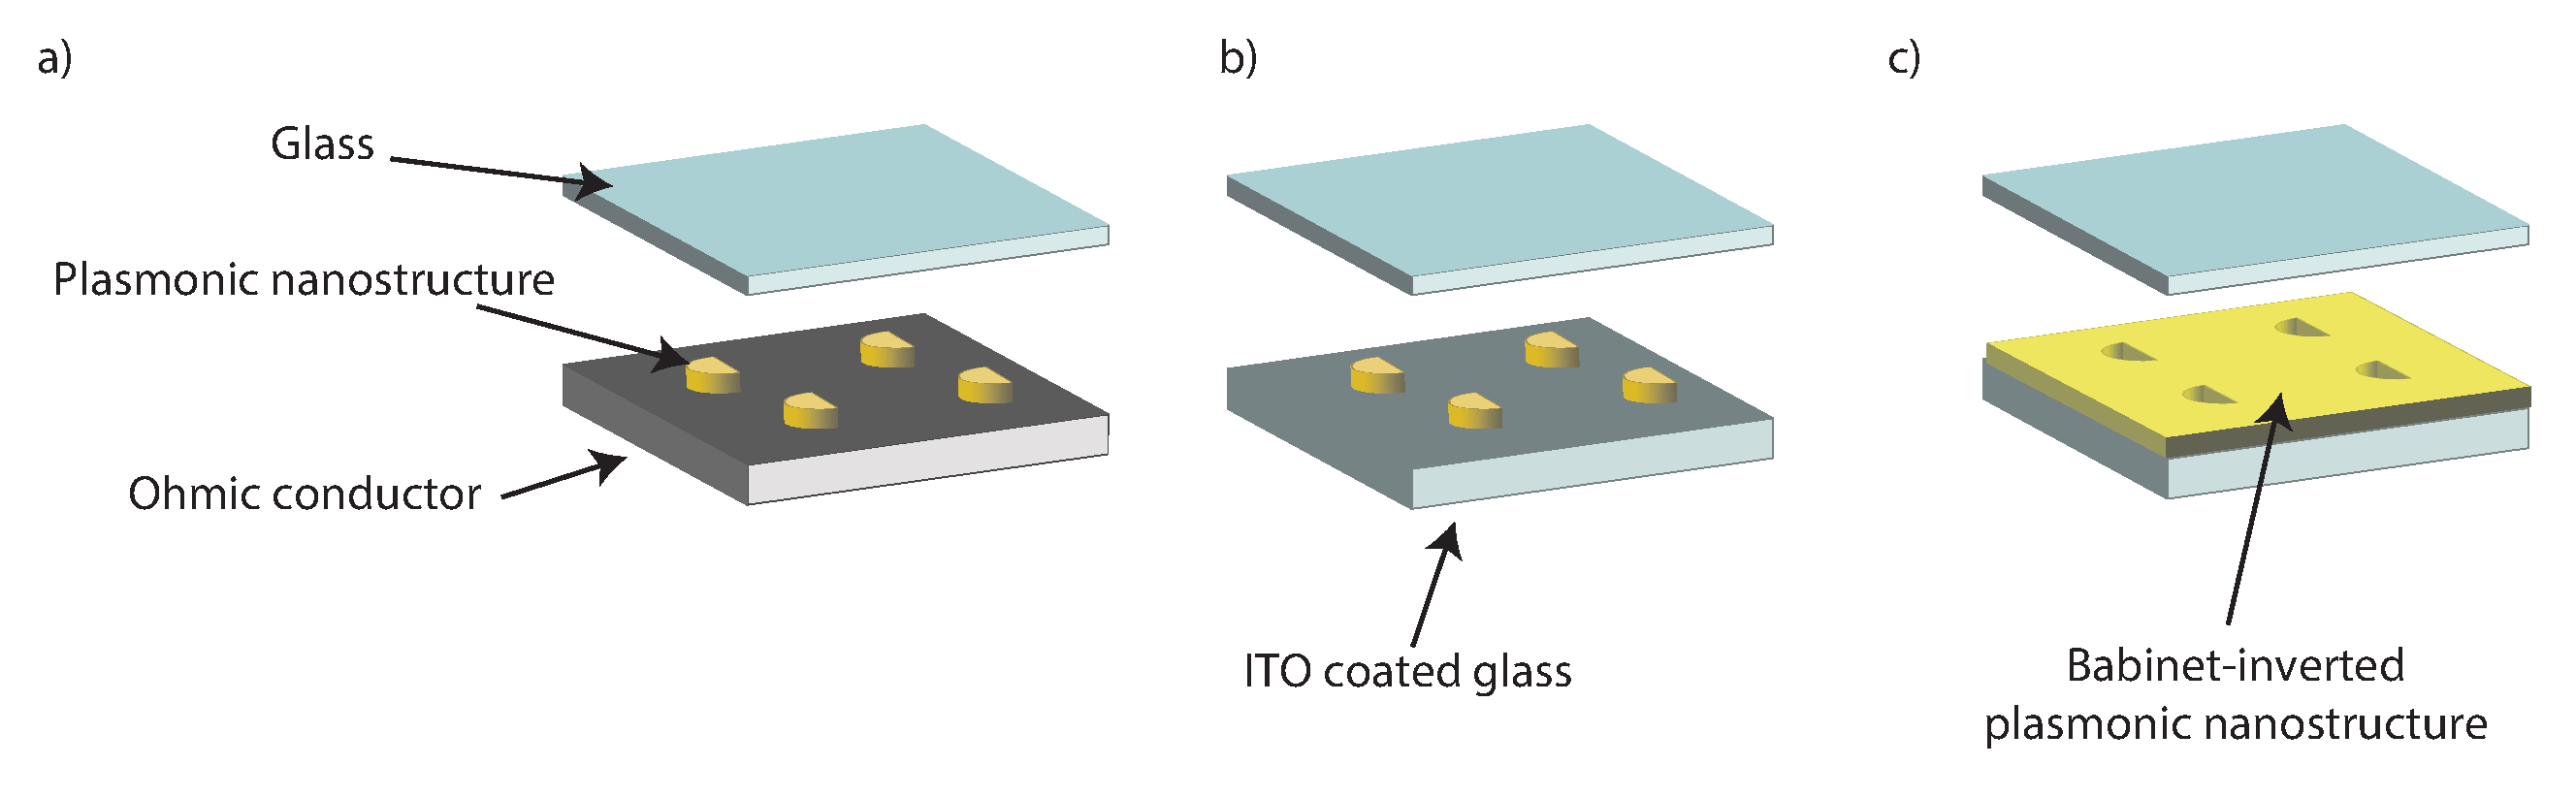
\includegraphics[width=\textwidth]{3Schem2.pdf}
%\caption{Device schematic}
%\label{Schem}
%\end{figure}
\par The patterns are created in Adobe Illustrator since the dimensions of the objects are accurately input. Adobe Illustrator also has the feature of exporting to DXF and DWG files. These files are compatible with the BEAMER software that is provided at Brookhaven National Lab to create the patterns compatible with the electron beam lithography machine.
\begin{figure}[h!]
\centering
\tikz[baseline=(a.north)]\node[yscale=-1,inner sep=0,outer sep=0](a){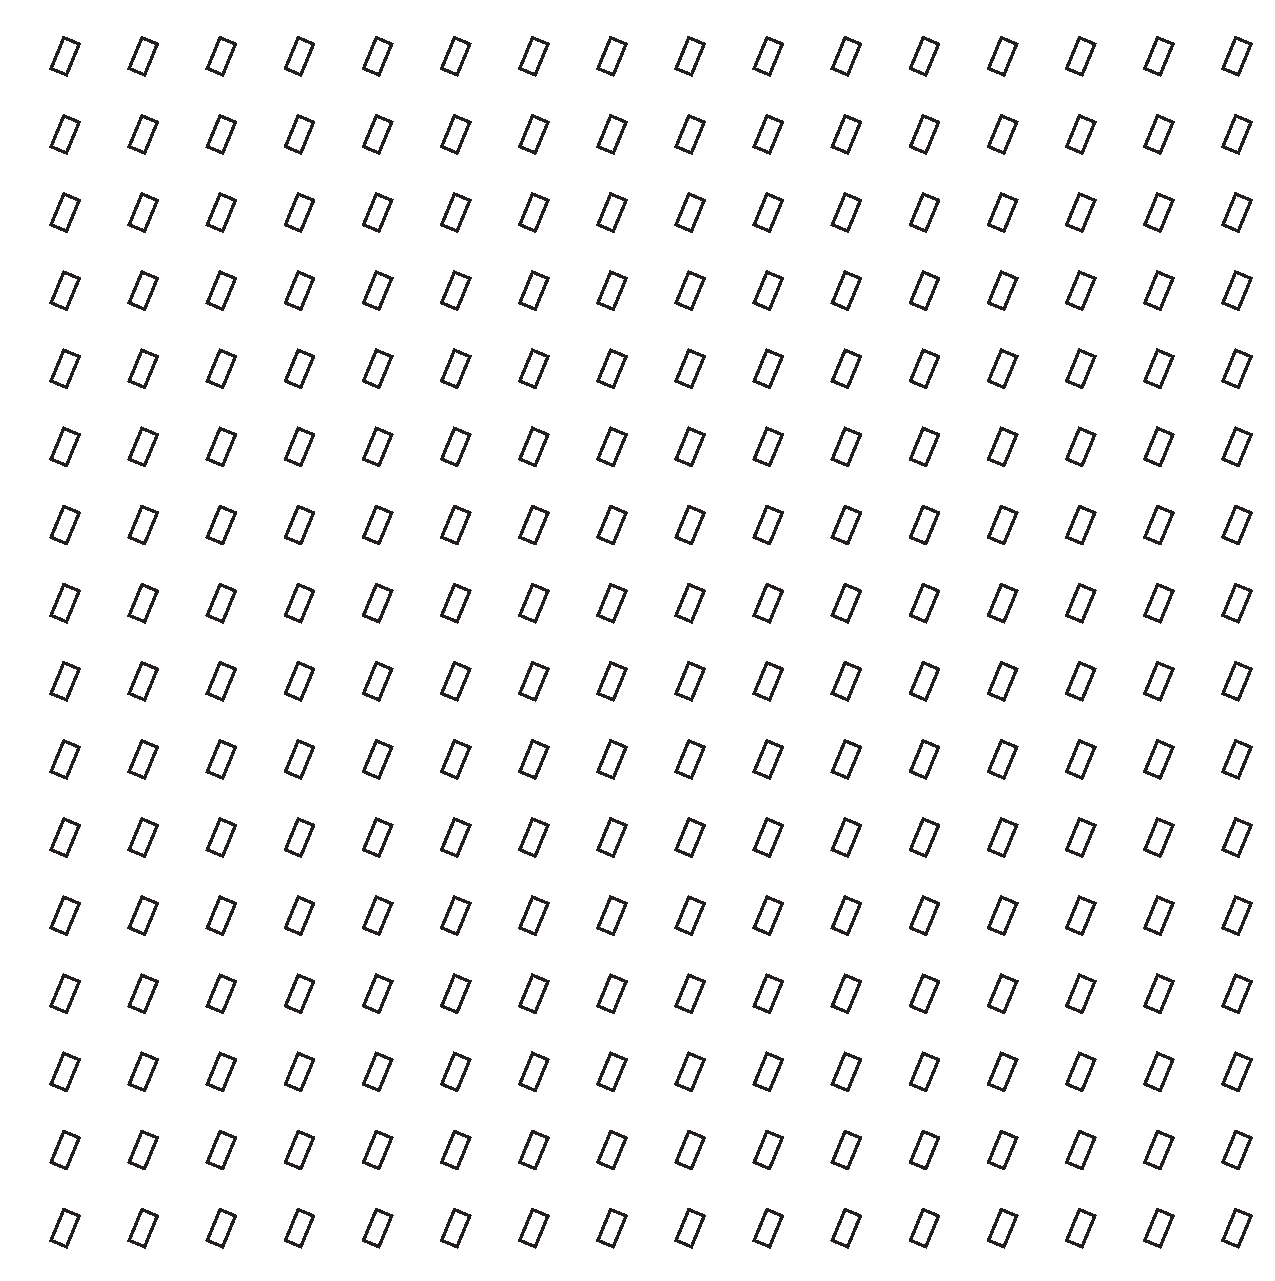
\includegraphics[width=0.75\textwidth, angle = 90]{ApertureRodDesign.pdf}};
\caption{Electron beam lithography pattern, nanoapertures measure 80nm by 160nm in a square lattice with periodicity between the structures measuring 375nm.}
\label{EbeamPattern}
\end{figure}
\subsection{Development}
\subsubsection{Electron beam resist}
The electron beam resist used was ZEP-520A, the resist thicknesses as a function of spin speed and dilution has been studied elsewhere [\cite{SpinCurve}], the thickness data is given as follows in Fig. ~\ref{spinCurve}. ZEP-520A has the properties of showing very high resolution. This is important for this work since the structures that will fabricated are on the order of 10$^{-8}$m (10nm), and thus the electron beam resist needs to show the greatest contrast for the nanostuctures to be well defined and have the desired optical properties. 

Another common electron beam resist that was considered is PMMA. PMMA is the most common electron beam resist used since it offers high resolution, is easy to handle and film characteristics have been well-studied. Though, like ZEP-520A, PMMA also provides high resolution it exhibits low contrast, which could lead to undesired optical properties.

Characteristics of ZEP-520A, are that it has a positive tone, resolution of at least 20nm, has a dry etch resistance similar to many photo resists. The film life, however is relatively short compared to other electron-beam resists such as PMMA.
\begin{figure}[h!]
\centering
\includegraphics[width=0.75\textwidth]{ZEP520a_spincurve.png}
\caption{Spin curve for ZEP-520A. \\Image: https://ebeam.mff.uw.edu/ebeamweb/process/ process/zep520a.html}
\label{spinCurve}
\end{figure}
\subsubsection{Fracturing}
The shot pitch of the electron beam lithography machine is set to 0.125nm. Since at some points of the structure the shot pitch is not exactly divisible by the shape size, the dimensions of the shape produced may be slightly off (by a maximum of one shot pitch)  To solve this problem shot pitch fracturing is enabled, such that some extra pixels are overlapped and the correct dimensions specified are achieved [\cite{BEAMER}]. This is important in fabricating the structures since they have very small feature sizes. Plasmonic effects are highly sensitive to structure dimensions, thus, shot pitch fracture is necessary to retain the specific dimensions of the nanostructures, and by relation the plasmonic response is preserved.
\subsubsection{Proximity effect correction}
Electron beam lithography can often make sharp corners rounded. The reason for this is due to scattering of the electron beam in the resist and substrate leading to undesired resist etching in the proximity of the beam, known as the proximity effect [\cite{PEC}]. Though the individual shapes are the same size the edges of nanostructures are likely to experience the proximity effect.

One way to use proximity effect correction is via dose modulation, in which each individual shape in a pattern is given a dose such that the shape prints the correct size. Generally, the proximity effect can be thought of as larger-patterned areas receive larger doses due to the electron scattering. To compensate the larger areas receive slightly lower dosages, or alternatively, the smaller areas receive slightly higher dosages.

Another method to resolve the proximity effect is via pattern biasing. In this method the larger dose that greater area patterns receive from the proximity effect is compensated by making the area either smaller or less dense. 

%\begin{figure}[h!]
%\centering
%\includegraphics[width=0.5\textwidth]{EBeamPattern2.png}
%\caption{Electron beam lithography pattern}
%\label{EbeamPattern2}
%\end{figure}
\subsubsection{Developers}
There are a number of different developers available for use. Xylenes are a common developer since the dosage needed is low, so patterns can be written faster, however the contrast is generally low. Amyl-acetate has a higher contrast, and hexyl-acetate has the highest contrast. Though the higher the contrast, the higher dosage generally needed to write the pattern and develop effectively. Contrast can b further improved by developing at low temperature.\\

\subsection{Recipe}
The recipe of rod-shaped nanoapertures is as follows:
First on a glass substrate a 3-nm wetting layer of chromium was deposited, followed by a 30-nm layer of gold with an electron beam evaporator. The thicknesses of the layers were accurately measured via a Filmetrics F20-UV thin film analyzer. From an initial test sample the rates of the electron beam evaporator were accurately determined to produce reliable film thicknesses. The rates of chromium and gold were deposited at a rate of 0.4$\AA$ per second to produce film with high uniformity and low surface roughness($<$2nm).

Next a layer of ZEP 520a is spin-coated onto the sample. The thickness of which is determined by the thickness of gold and the ion-milling rates of both gold and ZEP 520a. Since the desired result is a gold film with rod-shaped apertures that propagate the entire thickness of the film, once the pattern is written on the resist, and developed, there will be rod-shaped apertures in the resist. At the ion-milling stage, where the pattern is written gold is exposed to the ion miller and will be milled away, everywhere else only the resist is exposed to the ion miller and will be milled. Ideally, as the resist is milled away, and the gold is milled away where the pattern is written, once the entire layer of resist is completely milled away, so is the gold, where the pattern is written. Therefore the layer of resist that needs to be spin-coated is equal to:
\begin{equation}
L_{ZEP} = \frac{MR_{Au}}{MR_{ZEP}}\times L_{Au},
\end{equation}
where $MR_{AU}$ is the milling rate of gold, $MR_{ZEP}$ is the milling rate of the resist, ZEP 520a, $L_{Au}$ is the layer thickness of gold, and $L_{ZEP}$ is the layer thickness of ZEP 520a.

Using test samples of substrates with gold and spin-coated ZEP 520a, by measuring the thicknesses of the respective layers both before and after a specified time of ion-milling, the milling rates for both gold and ZEP 520a were determined to be approximately 0.1$\AA/s$ and 1.0$\AA/s$ respectively. With a gold layer thickness of 30nm, the layer of ZEP 520a that was spin-coated necessarily had to be at least 300nm. In this way, in the ion milling process the layer of resist will be completely milled away at the same time that the gold will be milled away where the pattern is written. Fig.~\ref{spinCurve} shows that for a 1:1 dilution of ZEP 520a the spin speed should be approximately around 500rpm for the desired 300nm film thickness.
\begin{figure}[h!]
\centering
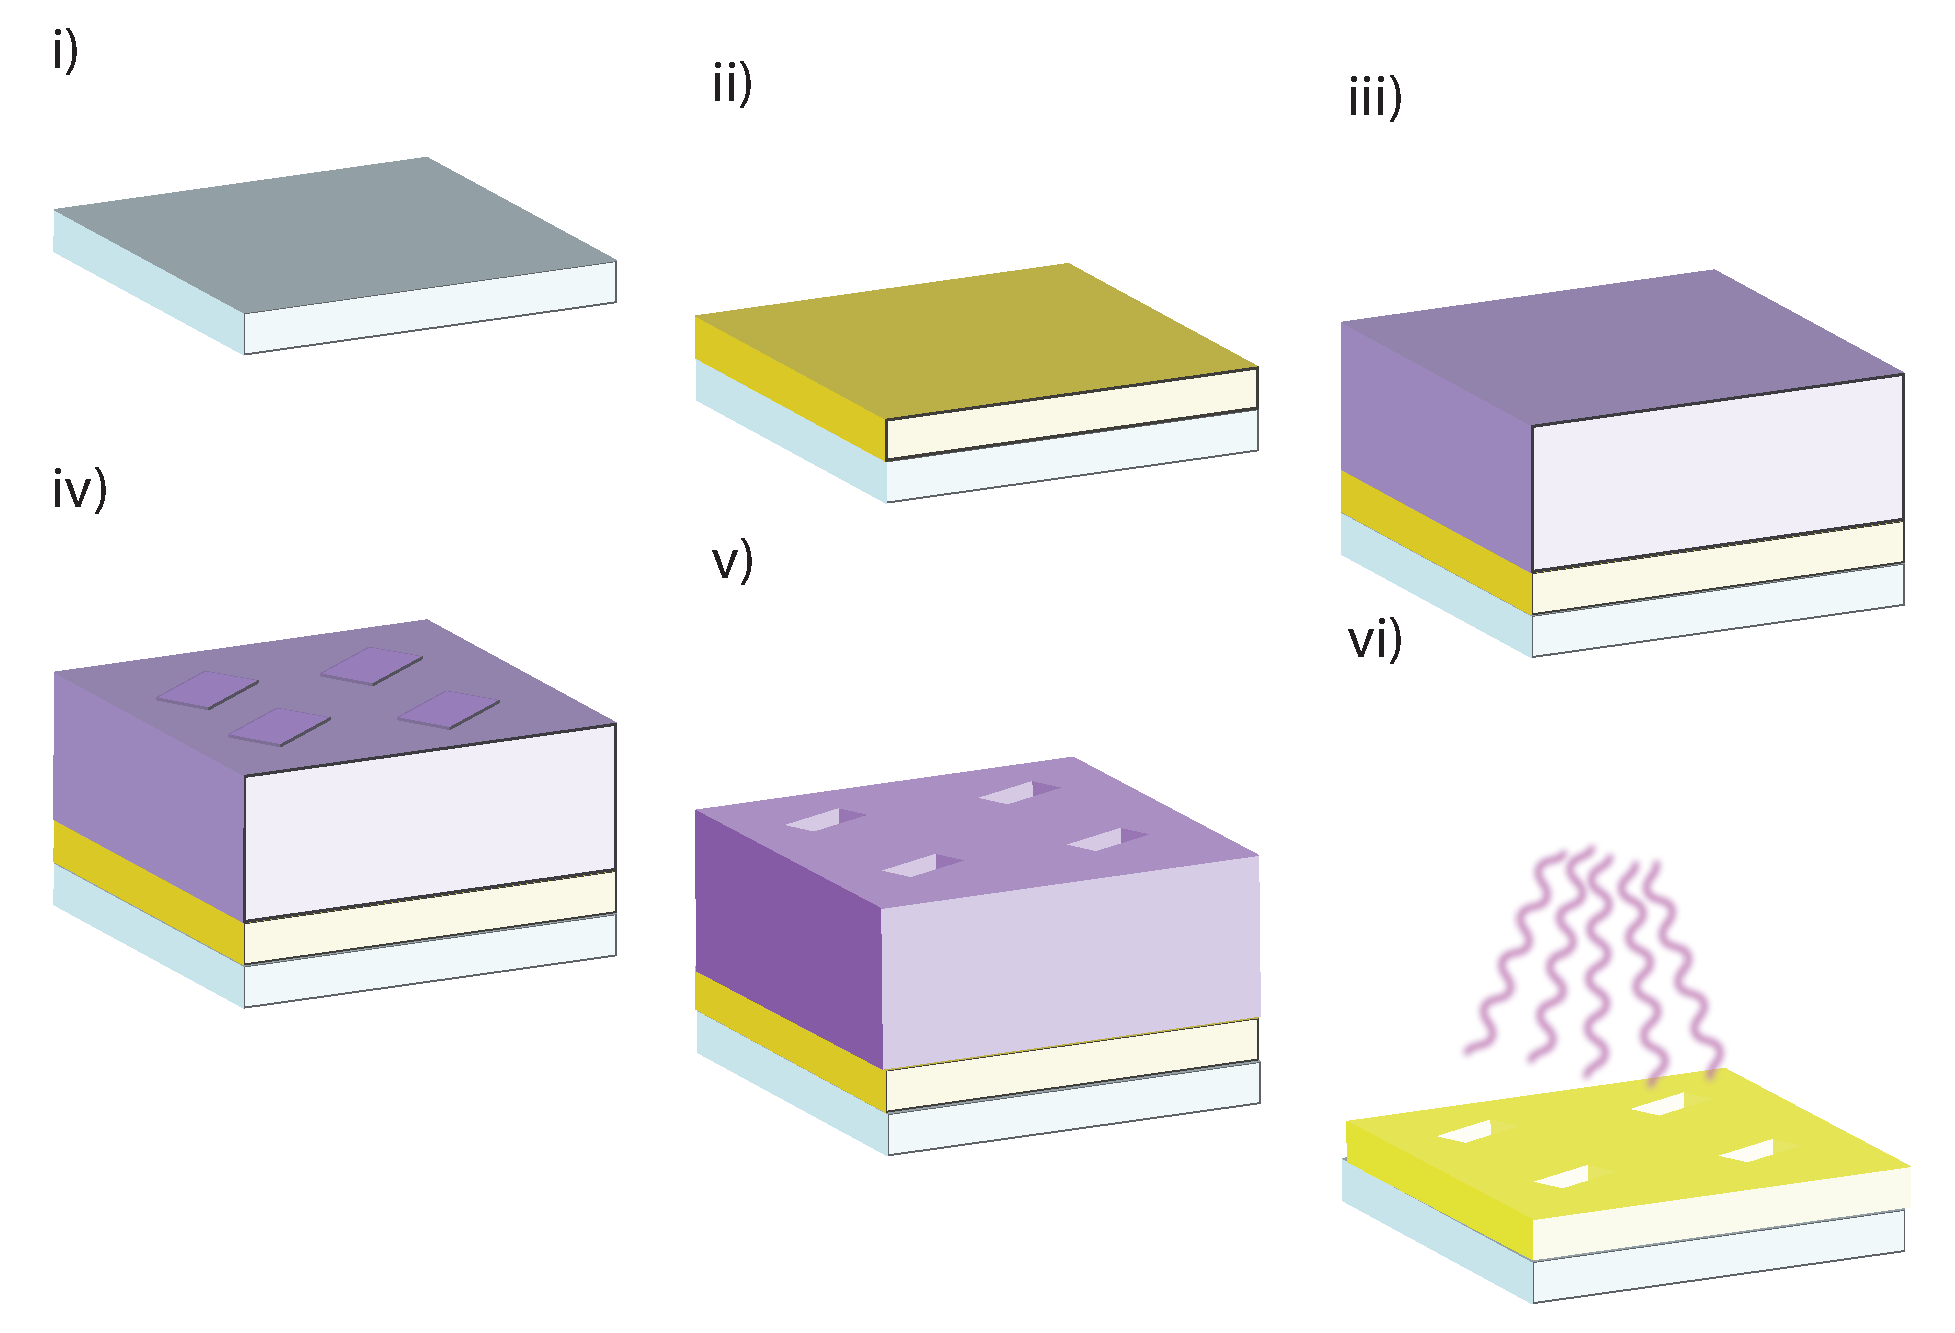
\includegraphics[width=0.9\textwidth]{NanoApertureRecipeRods.pdf}
\caption{Recipe to fabricate nanoapertures. i) Glass substrate, ii) gold layer is deposited, iii) ZEP 520a electron beam resist is deposited, iv) pattern is written via electron beam lithography, v) pattern is developed, vi) resist and gold is milled away}
\label{NanoApertureRecipe}
\end{figure}

Following, a 1.5mm $\times$ 1.5mm area pattern is written on the resist with the electron beam lithography machine. A via trial-and-error a dosage of $500\mu C/cm^2$ was used. Trial-and-error was performed by setting a variety of dosages, running the pattern, developing, and inspecting under a scanning electron microscope to determine which particular dosages were under/over-exposed, and which worked best. In the same way the current of the electron beam was determined to be 250pA.% on mode 6. Lower currents allowed for smaller patterns to be written which was needed for the smaller feature sizes and 250pA is a relatively small current. Mode 6 is used opposed to mode 3 for the smaller allowed shot pitch, 0.125nm for mode 6, opposed to 2nm for mode 3. Before each pattern is written the machine is calibrated to ensure the machine is optimal.\\

Once the pattern is written the sample was developed, hexyl-acetate was determined to be the best developer due to its high contrast especially at low temperature conditions. The sample was developed in hexyl-acetate at -25$^oC$ in a propylene glycol bath for 90 seconds followed by a rinse in iso-propyl alcohol.\\
Finally the sample was ion-milled such that the remainder of the resist is removed. The sample was visually inspected for any resist. The resulting metasurface is shown in Fig.~\ref{fig:rotlin}(a) as a scanning electron microscope image viewed from above. 
\begin{figure}[t!]
\centering
\includegraphics[width=0.7\linewidth]{bothSchem.eps}
\caption{The schematic diagram for (a) transmission measurements and (b) polarization measurements.}  
\label{fig:schematics} 
\end{figure}
\subsection{Transmission measurement setup}
To measure the optical chirality from the metasurface a xenon solar simulator is employed that provides stable broadband illumination between 400nm and 1000nm. The polarization state of light is controlled with a wire grid polarizer a 400-nm to 800-nm achromatic quarter-wave plate. The spectrum from the sample is captured via a CCD-coupled spectrometer [Fig.~\ref{fig:schematics}(a)].  

\subsection{Polarization measurement setup}
The eigen-polarization states are determined in a similar setup described above, however a spectral filter is used and the CCD-coupled spectrometer is replaced with a polarimeter to determine the polarization of transmitted light [Fig.~\ref{fig:schematics}(b)].

\section{Experimental difficulties and future work}
It has been demonstrated that chiral phenomena exists in regular arrays of rod-shaped nanoapertures tilted at 22.5$^\circ$. To further establish this phenomena, arrays of nanoapertures may be fabricated with varying tilt angles and periodicities. Variation of the periodicity would affect the coupling between nanostructures, and variation of the tilt angle would vary the strength of the perpendicular force generated that leads to the chiral phenomena observed.

The same effect may also be achieved with nanostructures, i.e., the non Babinet-inverted structure. The recipe for this type of metasurface was attempted however, due to the lift-off step, which can be quite difficult to perform, this type of metasurface was not pursued. The type of metasurface is fabricated in much the same manner as the one investigated, however the gold film is deposited after the electron beam lithography process. This makes the fabrication challenging as the non-conductive property of the glass substrate creates a difficult environment to perform the electron beam lithography.

Future work may also involve exploration into the optical forces that arise with the chiral phenomena, named optical rectification. Transverse Lorentz forces arise when light is illuminated on the metasurface [\cite{Proscia}] that are realised as a transverse voltage which are theoretically measurable on this metasurface. Moreover due to the non-centrosymmetric pattern that the rod-shaped nanoapertures exhibit when tilted at angles such as that studied here, $\theta_s=22.5^\circ$, the transverse voltages should exist even at normal incidence. These measurements typically require intense pulsed laser fields ($>$1MW/cm$^2$) and sensitive voltage measurement instruments.

Preliminary work was performed in the area of chiral responses and transverse voltages from other shapes, namely semi-circles or D-shapes. These shapes differ from the rectangular, rod-shapes studied here in that the the fundamental shape is non-centrosymmetrical, the shape can only can only be superimposed in rotation of $n\times 2\pi$ radians, where $n$ is an integer. The rod-shapes however are identical when rotated by $n\times \pi$ radians. Arrays of both shapes, when placed in an array cannot be titled at an angle $m\times \pi/4$ radians, where $m$ is integers including 0, otherwise symmetry is not broken. If the shapes are tilted prescribed by the condition above chiral phenomena occurs at normal incidence. The phenomena is much weaker in magnitude at normal incidence than structures optimized for oblique incidence but serves a much more general method to achieve chiral phenomena in metasurfaces. 
\clearpage

% Summary
\chapter{Summary and Outlook}
\chaptermark{Summary and Outlook}
\section{What has been done}
This thesis has discussed the manipulation of optical properties and optically-generated forces of plasmonic nanoparticles. The light-matter interactions studied here range from the magneto-optical responses that are exhibited in gold nanoparticles to the spatial encoding of information via fractal architectures, and ultimately contribute to the next generation of metamaterials and metasurfaces. The applications optically-generated forces on nanoparticles can influence the future fabrication processes of metamaterials and metasurfaces. While top-down fabrication techniques, typically used to fabricate such devices, offer excellent nanometer-precision of the arrangement of individual features. Generally, only small areas can be patterned at a time ($<$10cm$^2$), and suffer from limitations such as the need for expensive machines and long fabrication time. For widespread adoption of these materials bottom-up fabrication techniques must ultimately be developed. The work in this thesis studies the optical forces on the plasmonic nanostructures, often the building blocks of metamaterials and metasurfaces, is the first step in the development of bottom-up fabrication of these structures. Also studied are the applications of metasurfaces which include increased and robust data transmission rates, and a demonstration of their versatility via the fabrication of a chiral metasurface by the arrangement of non-chiral sub-structures.

The light-matter interactions studied here are derived from plasmonic excitations that occur when light is incident on metallic nanoparticles. Plasmonic interactions are popular for a variety of factors including high local field confinement, and enhancement of nonlinear phenomena [\cite{Novotny2011, Kauranen}]. Popularity of plasmonic materials also stems from their sensitivity to the optical properties the metal and dielectric materials that compose the interface of which plasmons are created [\cite{Homola}].

In chapter 2 magneto-optical effects are demonstrated in gold nanoparticles. The nanoparticles are illuminated by circularly-polarized light which generate plasmon-assisted solenoidal currents that flow on the surface of the nanoparticles. The solenoidal currents magnetize of the nanoparticles according to Faraday's law, which is observed experimentally via the extinction spectra.

In chapter 3 the Lorentz force is investigated when nanowires are illuminated with plane waves at oblique incidences. The plasmonic modes that are excited on the nanowire induce forces and torques that explain the rocking and spinning motion that other experimental scientists have observed, yet have been previously unexplained.

In chapter 4 chirality is shown in a metasurface composed of non-chiral substructures, namely rod-shaped apertures.  The chirality is present occurs due to interactions between neighbouring substructures that is derived from the Li\'{e}nard-Wiechert potential, and is observed experimentally via the change in polarization through the metasurface. The polarization exhibits optical rotation and circular dichroism at normal incidence\textemdash the signature of chiral phenomena. Developing chiral media is important for applications where either accurate control over the polarization is desired or for the development of a new generation of polarization detectors [\cite{Mueller:16}].

Chapter 5 shows that information is encoded robustly when designed and transmitted with fractal architecture. Self-similar transmission profiles are less sensitive to intermediate-obstacle signal blocks and are regenerated easily without distortion of the original image. Applications of this work may be relevant to any large-scale data transmission platforms.


\section{What is left to do}
%One of the limitations of nanofabrication is the necessity for extremely expensive machines that make research inaccessible to many. 
One of the future goals of the research studied in this thesis is to develop new methods to self-assemble structures at the nanoscale. Understanding how Lorentz forces are generated at the nanoscale is unintuitive, yet fundamental to fabricating consistent, uniform, defect-free nanostructures at scale. Further explorations into this topic may investigate methods to validate the magnitudes, directions, and locations of Lorentz forces when light is applied to nanostructures. 

%Challenges in the experimental verification occur in a number of ways, from the optical trapping of nanostructures, to confinement of light at the orders similar to the wavelength. Regardless, the highly diverse nature of plasmonics presents an exciting future, where, for example the development of ultrafast computing, active plasmonic devices or biochemical applications.

Control over the polarization has been explored here through the use of a chiral metasurface. It is a goal of scientists to probe the nature of materials via various optical characterization methods. This work began by simply observing the scattering and absorption properties [\cite{Mie}], which later gave rise to spectrophotometry. Optical characterization techniques since grown to include methods such as Fourier transform infra-red spectroscopy [\cite{Chan:2016}], ellipsometry [\cite{Theeten:1981}] and surface enhanced Raman spectroscopy [\cite{Wang:2015}]. To this end, materials that are able to efficiently modify the polarization fields of light to probe a materials properties such as the structure or composition are extremely desirable. Metasurfaces are one way of achieving efficient polarization control, they modify the polarization over length scales smaller than the wavelength. For comparison, traditional polarization optics need length scales around 3 orders of magnitude greater than the wavelength, such as polarizers, and quarter wave-plates, making metasurfaces very attractive in this regard.

One area of improvement that can be made in the development of future metasurfaces is reconfigurability. Similar to how a spatial light modulator is able to manipulate the phase, the same can be achieved with metasurfaces. The work presented as part of this thesis lays out methods to optically manipulate either metallic nanoparticles (chapters 2, 3) or the polarization (chapter 4). It is conceivable that future applications of the work studied here may combine the two, optically arranging metallic nanoparticles on a large scale using Lorentz forces derived from the plasmonic interaction, into some metasurface configuration [\cite{Aieta}], or even the fractal geometries explored in chapter 5. The metasurface could demonstrate its function, manipulating the polarization of light. Following, the metasurface may be reconfigured for another purpose or function. Challenges in this area will involve uniform fabrication\textemdash any irregularities may give rise to structural correlations that lead to unwanted effects, or nonlocal effects at the nanoscale. Challenges may also be faced in having to overcome any optical losses associated with metallic nanoparticles, where dielectric materials may be more desirable.

The complete control over structures at the nanoscale is highly attractive and has the potential to usher an era of large-scale manufacturing of materials to probe the fundamentals properties of materials. Metallic nanoparticles can act as the building blocks of metasurfaces and metamaterials, not only can their size, shape, and composition be modified, but their spatial arrangement can lead to more complicated and precise control over light, from intensity to colour to polarization. This thesis represents a few small progressions to these goals.

\chapter{Appendix}
\chaptermark{Appendix}

\section{Matlab function code to create Sierpinski carpet hologram}
\lstset{language = Matlab}
\begin{lstlisting}
function carpetHolo = Sierpinski(fracOrder);
	carpetBase = ones(3); % Initialize matrix
	carpetBase(2,2) = 0;
	% Zero middle element
	if fracOrder==0;
		% For zero order case
		carpetHolo = carpetBase;
	else
		% For higher order cases
		carpetHolo= kron(carpetBase,carpetBase);
		% For loop iterates the Kronecker tensor product
		for i = 1:fracOrder-1
			carpetHolo = kron(carpetHolo,carpetBase);
		end
	end
end
\end{lstlisting}

\section{Matlab function code to recreate Sierpinski carpet hologram}

\begin{lstlisting}
function recon = reconFun(Threshold,carpetBaseLength,carpetHolo)
	% Ratio of length of hologram
	normLength = length(carpetHolo)/carpetBaseLength; 
	
	% Convert to array of cells
	cellHolo = mat2cell(carpetHolo,repmat(normLength,1,...
	carpetBaseLength),repmat(normLength,1,carpetBaseLength));
	
	% Calculate mean, determine if above threshold value, and plot
	pcolor(double(cell2mat(cellfun(@mean2, cellHolo))>Threshold));
end
\end{lstlisting}



\chapter*{Previously Published Materials}
\label{chap:ppm}
\addcontentsline{toc}{chapter}{\nameref{chap:ppm}}
\nobibliography* 
The content of this dissertation is based substantially on material previously published by Matthew Moocarme and colleagues. This includes in particular the list of journal articles below.
\vspace{5mm}

\noindent
\bibentry{Moocarme2014}
\vspace{5mm}

\noindent
\bibentry{Moocarme14}
\vspace{5mm}

\noindent
\bibentry{Moocarme15}
\vspace{5mm}

\noindent
\bibentry{Moocarme16}


%\import{../../Research/Four/Paper/}{Tables}
\clearpage
%\import{../../Research/Four/Paper/}{Tables_appendix}
\clearpage


% end matter
\singlespacing
\bibliographystyle{apalike}
\bibliography{../refs}

\end{document}
